\documentclass[]{aa}

\usepackage{graphicx}
\usepackage{txfonts}
\usepackage{natbib}

\bibpunct{(}{)}{;}{a}{}{,} % to follow the A&A style


% shortcut to typeset a 2x2 matrix... we do a lot of these
\newcommand{\matrixtt}[4]{\left( \begin{array}{cc}#1&#2\\#3&#4\\\end{array} \right)}

% typographical conventions
% this typesets a Jones matrix
\newcommand{\jones}[2]{\vec {#1}_{#2}}
% this typesets an inverse Jones matrix
\newcommand{\jonesinv}[2]{\vec {#1}^{-1}_{#2}}
% this typesets a conjugate-transpose Jones matrix
\newcommand{\jonesT}[2]{\vec {#1}^\dagger_{#2}}
% this typesets an inverse conjugate-transpose Jones matrix
\newcommand{\jonesTinv}[2]{\vec {#1}^{\dagger-1}_{#2}}
% this typesets a coherency matrix
\newcommand{\coh}[2]{\mathsf{{#1}}_{{#2}}}

\begin{document}


\title{Revisiting the Measurement Equation: Understanding And Calibrating Direction-Dependent Effects  In Radio Interferometers}

\author{O.M.\ Smirnov}

\institute{Netherlands Institute for Radio Astronomy (ASTRON)\\
  P.O. Box 2, 7990AA Dwingeloo, The Netherlands \\
  \email{smirnov@astron.nl}}

\date{}

\titlerunning{Measurement Equation \& Direction-Dependent Effects}
\authorrunning{O.M.\ Smirnov}

\abstract%
%context
{This is a placeholder abstract.}%
%aims
{World domination.}
%methods
{Promote the Measurement Equation.}%
%results
{I've had a few // but then again...}%
%conclusions
{World domination via the M.E. is imminent.}

\keywords{Methods: numerical - Methods: data analysis - Techniques:
interferometric - Techniques: polarimetric}

\maketitle

\section*{Introduction}

The Measurement Equation of a generic radio interferometer (henceforth referred to as RIME. ``The Measurement Equation'' is also a term in current use, but seems overly broad.) was formulated by \citet{ME1} after almost 50 years of radio astronomy. Prior to the RIME, mathematical models of radio interferometers (as implemented by a number of software packages such as AIPS, Miriad, NEWSTAR, DIFMAP) were somewhat ad hoc and approximate. Despite this (and in part thanks to the careful design of existing instruments), the technique of {\em selfcalibration} \citep{Cornwell:selfcal} has allowed radioastronomers to achieve spectacular results. However, by the time the RIME was formulated, even older and well-understood instruments such as the WSRT were beginning to expose the limitations of these approximate models. New instruments (and upgrades of older observatories), such as the current crop of Square Kilometer Array \citep{Schilizzi:SKA} ``pathfinders'', and indeed the SKA itself, were already beginning to loom on the horizon. These new instruments exhibit far more subtle and elaborate observational effects, due not only to their greately increased sensitivity, but also to new features of their design. In particular, while traditional selfcal only deals with direction-independent effects (DIEs), calibration of these new instruments requires us to deal with Direction-Dependent Effects (DDEs), that is, effects that vary across the field of view (FoV) of the instrument. 

It is then quite fortunate that the emergence of the RIME formalism has provided us with a complete and elegant mathematical framework for dealing with observational effects, and ultimately DDEs. Oddly enough, outside of a small community of algorithm developers that have enthusiastically accepted the formalism and put it to good use, uptake of RIME by radio astronomers at large has been slow. Anecdotal evidence suggests that some of the ``old guard'' either perceives the RIME as arcane and unnecessary, or simply fails to see its benefits. Even more worryingly, almost 15 years after the first publication, the formalism is not taught to the new generation of students. Worryingly, because in the author's estimation, the RIME should be the cornerstone of every entry-level interferometry course!\footnote{Section~\ref{sec:what-is-the-point} discusses this assertion in depth.} In part this slow acceptance has been shaped by the availability of software. Today's radio astronomers rely almost exclusively on the software packages mentioned above, whose internal paradigms are rooted in the selfcal developments of the 1980s and lack an explicit RIME.\footnote{All legacy packages do use some specific and limited form of the RIME implicitly. This will be discussed further in Sect.~\ref{sec:implicit-mes}.} The continued success of legacy packages means that the {\em thinking} about interferometry and calibration is still largely shaped by pre-RIME paradigms. It doesn't help that new software exploiting the power of the RIME has been slow to emerge, and practical results even more so (but see Sect.~\ref{sec:3C147} of this paper.)  

On the other hand, from the author's personal experience of teaching the RIME at several workshops, once the penny drops, people tend to describe the RIME in terms such as ``obvious'', ``simple'', ``intuitive'', ``elegant'' and ``powerful''. This suggests that there's an explanatory gap in the literature. The first part of this paper therefore tries to address this gap, recasting existing ideas into one consistent mathematical framework, and showing where other approaches to the RIME fit in. Section~\ref{sec:derivation} revisits the ideas of the original RIME papers I and IV \citep{ME1, ME4}, deriving the RIME from first principles. It then shows how fundamentals of interferometry itself (and the van Cittert-Zernike theorem in particular) follow from the RIME (rather than the other way around!), in the process showing how the formalism incorporates DDEs. Section~\ref{sec:formulations} looks at alternative formulations of the RIME and their practical implications, and shows where they fit into the formalism. It also tries to clear up some controversies and misunderstandings that have accumulated over the years. Section~\ref{sec:what-is-the-point} then discusses why the RIME is crucial in the context of modern and future instruments (with the benefit of 15 years of hindsight.) Section~\ref{sec:calibration} discusses calibration in RIME terms, and explicates the links between the RIME and various legacy implementations of selfcal. 

The second half of this paper deals with the subject of DDEs, which were not covered by the original RIME formulation at all. Typical DDEs are caused by beamshapes that are variable in time and/or different between antennas, pointing errors (which could be considered a simple case of differing beamshapes), ionospheric and tropospheric refraction, etc. The problem of DDEs is two-pronged: firstly, some effects are not known apriori and must therefore be calibrated for directly from the data, and secondly, even when the effect is known, correcting for it is decidedly untrivial. A lot of progress has been made on the latter problem, and \citet{SB:imageplane} have proposed an algorithm that corrects for known DDEs during imaging and deconvolution. \citet{Rau:DDEs} and \citet{SB:calibration-low-freq} provide an in-depth review of other developments. This paper will concentrate on the calibration aspect of the problem.

The above authors have developed a description of DDEs using the $4\times4$ Mueller matrix and coherency vector formalism of \citet{ME1}. The $4\times4$ formalism has also been included in the 2nd edition of \citet*[Sect.~4.8]{tms}. In the meantime, \citet{ME4} has recast the RIME using only $2\times2$ matrices. The $2\times2$ form of the RIME has far more intuitive appeal,\footnote{This admittedly subjective judgement is firmly based on the author's teaching experience.} and is far better suited for describing calibration problems, yet has been somewhat unjustly ignored in the literature. Addressing this perceived injustice is yet another aim of this paper. (Section~\ref{sec:formulations} describes the $4\times4$ vs. $2\times2$ formalisms in more detail.)

Section~\ref{sec:ddes} of this paper presents an analysis of the DDE problem using the $2\times2$ formalism. Sect.~\ref{sec:dde-examples} talks about some specific DDEs relevant to current and future instruments, and shows some instructive simulations of these DDEs using the MeqTrees software \citep{meqtrees}. Last but certainly not least, Sect.~\ref{sec:3C147} shows an application of these concepts to real data. It presents a record dynamic range (over 1.5 million) calibration of a WSRT observation, including calibration of DDEs, and discusses the implications of this result for the calibratability of future telescopes such as the SKA.

\section{\label{sec:derivation}Revisiting the Measurement Equation}

\subsection{The RIME of a single source}

\subsubsection{Signal propagation}

Consider a single source of quasi-monochromatic signal (i.e. a sky consisting of a single point source.) The signal at a fixed point in space and time can be then be described by the complex vector $\vec e$. Let us pick an orthonormal $xyz$ coordinate system, with $z$ along the direction of propagation (i.e. from antenna to source.) In such a system, $\vec e$ can be represented by a column vector of 2 complex numbers:

\[
\vec e = \left( \begin{array}{c}e_x\\e_y\end{array} \right) 
\]

Our fundamental assumption is {\em linearity}: all transformations along the signal path are linear w.r.t. $\vec e$. Basic linear algebra tells us that all linear transformations of a 2-vector can be represented (in any given coordinate system) by a matrix multiplication:

\[
\vec e' = \jones{J}{} \vec e,
\]

where $\jones{J}{}$ is a $2\times2$ complex matrix known as the {\em Jones} matrix \citep{jones}. Obviously, multiple effects along the signal propagation path correspond to repeated matrix multiplications, forming what we call a {\em Jones chain}. We can regard multiple effects separately and write out Jones chains, or we can collapse them all into a single cumulative Jones matrix as convenient:

\begin{equation}\label{eq:jones-chain}
\vec e' = \jones{J}{n} \jones{J}{n-1} ... \jones{J}{1} \vec e = \jones{J}{} \vec e
\end{equation}

The order of terms in a Jones chain corresponds to the physical order in which effects occur along the signal path. Since matrix multiplication does not (in general) commute, we must be careful to preserve this order. 

Now, the signal hits our antenna and is ultimately converted into complex voltages by the antenna feeds. Let us further assume that we have two feeds $a$ and $b$ (for example, two linear dipoles, or left/right circular feeds), and that the voltages $v_a$ and $v_b$ are linear w.r.t. $\vec e$. We can formally treat the two voltages as a voltage vector $\vec v$, analogous to $\vec e$. Their linear relationship is yet another matrix multiplication:

\begin{equation}\label{eq:e-voltage}
\vec v = \left( \begin{array}{c}v_a\\v_b\end{array} \right) = \jones{J}{} \vec e
\end{equation}
 
Equation~(\ref{eq:e-voltage}) can be thought of as representing the fundamental linear relationship between the voltage vector $\vec v$ as measured by the antenna feeds, and the ``original'' signal vector $\vec e$ at some arbitrarily distant point, with $\jones{J}{}$ being the cumulative product of all propagation effects along the signal path (including electronic effects in the antenna/feed itself.) We shall call refer to this $\jones{J}{}$ as the {\em total Jones} matrix (as opposed to individual Jones terms in a Jones chain.) 

\subsubsection{The visibility matrix}

Two spatially separated antennas $p$ and $q$ measure two independent voltage vectors $\vec v_p,\vec v_q$. In an {\em interferometer}, these are fed into a correlator, which produces 4 pairwise correlations between the components of $\vec v_p$ and $\vec v_q$:

    \begin{equation}\label{eq:correlation}
    \langle v_{pa}v^*_{qa}\rangle, \langle v_{pa}v^*_{qb}\rangle, 
    \langle v_{pb}v^*_{qa}\rangle, \langle v_{pb}v^*_{qb}\rangle
    \end{equation}

Here, angle brackets denote averaging over some (small) time and frequency bin, and $x^*$ is the complex conjugate of $x$.  It is convenient for our purposes to arrange these four correlations into the {\em visibility matrix\/}\footnote{\citet{ME4} calls $\coh{V}{pq}$ the {\em coherency matrix}, in order to distinguish it from traditional scalar visibilities. Since the elements of the matrix are precisely the complex visibilities, we submit {\em visibility} matrix as a more logical term.} $\coh{V}{pq}$:

    \[
    \coh{V}{pq} = 2 \matrixtt{\langle v_{pa}v^*_{qa}\rangle}{\langle v_{pa}v^*_{qb}\rangle}{\langle v_{pb}v^*_{qa}\rangle}{\langle v_{pb}v^*_{qb}\rangle}
    \]

We introduce a factor of 2 here, for reasons explained in Sect.~\ref{sec:factor2}. It is easily seen that $\coh{V}{pq}$ can be written as a matrix product of $\vec v_p$ (as a column vector), and the conjugate of $\vec v_q$ (as a row vector):

\begin{equation}\label{eq:coherency}
\coh{V}{pq} = 2 \left<\left( \begin{array}{c}v_{pa}\\v_{pb}\end{array} \right) (v^*_{qa},v^*_{qb}) \right > = 2 \langle \vec v_p \vec v^\dagger_q \rangle
\end{equation}

Here, $\dagger$ represents the conjugate transpose operation (also called a Hermitian transpose.)

\subsubsection{\label{sec:RIME-emerges}The RIME emerges}

Starting with some arbitrarily distant vector $\vec e$, our signal travels along two different paths to antennas $p$ and $q$. Following eq.~(\ref{eq:e-voltage}), each propagation path has its own total Jones matrix, $\jones{J}{p}$ and $\jones{J}{q}$. Combining eqs.~(\ref{eq:e-voltage}) and (\ref{eq:coherency}), we get:

    \begin{equation}\label{eq:corr1}
    \coh{V}{pq} = 2 \langle  \jones{J}{p} \vec e ( \jones{J}{q} \vec e )^\dagger \rangle  = 2 \langle  \jones{J}{p} (\vec e \vec e^\dagger) \jonesT{J}{q} \rangle 
    \end{equation}

Assuming that $\jones{J}{p}$ and $\jones{J}{q}$ are constant over the averaging interval,\footnote{This is a crucial assumption, which we will revisit in Sect.~\ref{sec:smearing}} we can move them outside the averaging operator:

    \begin{equation}\label{eq:corr2}
    \coh{V}{pq} = 2 \jones{J}{p} \langle  \vec e \vec e^\dagger \rangle  \jonesT{J}{q} = 
    2 \jones{J}{p} 
    \matrixtt{\langle e_x e^*_x\rangle }{\langle e_x e^*_y\rangle }{\langle e_y e^*_x\rangle }{\langle e_y e^*_y\rangle }
    \jonesT{J}{q}
    \end{equation}

The bracketed quantities here are intimately related to the definition of the Stokes parameters \citep{born-wolf,tms}. \citet{ME3} explicitly show that

    \begin{equation}\label{eq:IQUV}
    2 
    \matrixtt{\langle e_x e^*_x\rangle }{\langle e_x e^*_y\rangle }{\langle e_y e^*_x\rangle }{\langle e_y e^*_y\rangle }
    = 
    \matrixtt{I+Q}{U+iV}{U-iV}{I-Q} = \coh{B}{}
    \end{equation}

We now define the {\em brightness matrix} $\coh{B}{}$ as the right-hand side\footnote{Following a long-standing controversy, we have decided to break with \citet{ME4} by omitting $\frac{1}{2}$ from the definition of $\coh{B}{}$, and adding a factor 2 to the definition of $\coh{V}{pq}$ in eq.~(\ref{eq:coherency}). The reasons for this will be spelled out in Sect.~\ref{sec:factor2}.} of eq.~(\ref{eq:IQUV}). This gives us the first form of the RIME, that of a single point source:

    \begin{equation}\label{eq:me0}
    \coh{V}{pq} = \jones{J}{p} \coh{B}{}  \jonesT{J}{q}
    \end{equation}

Or in expanded form:

\[
    \left( 
    \begin{array}{cc}
    v_{aa} & v_{ab} \\
    v_{ba} & v_{bb} \\
    \end{array}
    \right) = 
    \left( 
    \begin{array}{cc}
    j_{11p} & j_{12p} \\
    j_{21p} & j_{22p} \\
    \end{array}
    \right) 
    \left( 
    \begin{array}{cc}
    I+Q & U+iV \\
    U-iV & I-Q \\
    \end{array}
    \right) 
    \left( 
    \begin{array}{cc}
    j_{11q} & j_{12q} \\
    j_{21q} & j_{22q} \\
    \end{array}
    \right)^\dagger
\]

which quite elegantly ties together the observed visibilities $\coh{V}{pq}$ with the intrinsic source brightness $\coh{B}{}$, and the per-antenna terms $\jones{J}{p}$ and $\jones{J}{q}$.

Note that eq.~(\ref{eq:me0}) holds in any coordinate system. The vector $\vec e$, the brightness matrix $\coh{B}{}$ that is derived from it, and the linear transformations $\jones{J}{p}$ and $\jones{J}{q}$ are distinct mathematical entities that are independent of coordinate systems; choosing a coordinate basis associates a specific {\em representation} with $\vec e$,  $\coh{B}{}$ and $\jones{J}{}$, manifesting itself in a 2-vector or a $2\times2$ matrix populated with specific complex numbers. For example, it is quite possible (and sometimes desirable) to rewrite the RIME in a circular polarisation basis. This is discussed further in Sect.~\ref{sec:circular}. In this paper, we shall use an orthonormal $xyz$ basis unless otherwise stated.

\subsubsection{A note on typographical convention}

Throughout this paper, we shall adopt the following typographical conventions for formulae:

\begin{description}
\item[Scalar quantities] will be indicated by lower- and uppercase italics: $e_x,I,K_p$.
\item[Vectors] will be indicted by lowercase bold italics: $\vec e$.
\item[Jones matrices] willbe indicated by uppercase bold italics: $\jones{J}{}$. As a special case, scalar matrices
(Sect.~\ref{sec:taxonomy}) will be indicated by normal-weight italics: $K_p$.
\item[Visibility, coherency and brightness matrices] will be indicated by sans-serif font: 
$\coh{B}, \coh{V}{pq}, \coh{X}{pq}$. This emphasizes their different mathematical nature (and in particular, that they transform differently under change of coordinate frame, Sect.~\ref{sec:circular}).
\end{description}


\subsubsection{The ``onion'' form}

We can also choose to expand $\jones{J}{p}$ and $\jones{J}{q}$ into their associated Jones chains, as per 
eq.~(\ref{eq:jones-chain}). This results in the rather pleasing ``onion'' form of the RIME:

    \begin{equation}\label{eq:me0-onion}
    \coh{V}{pq} = \jones{J}{pn}(...(\jones{J}{p2} (\jones{J}{p1} \coh{B}{}  \jones{J}{q1}^\dagger)\jonesT{J}{q2}) ... )\jonesT{J}{qm}
    \end{equation}

Intuitively, this corresponds to various effects in the signal path applying sequential layers of ``corruptions'' to the original source brightness $\coh{B}{}$. Note that the two signal paths can in principle be entirely dissimilar, making the ``onion'' assymetric (hence the use of $n\ne m$ for the outer indices.) One of the strengths of the RIME is its ability to describe heterogenous interferometer arrays with dissimilar signal propagation paths.

\subsubsection{An elementary Jones taxonomy\label{sec:taxonomy}}

Different propagation effects are described by different kinds of Jones matrices. The simplest kind of matrix is a {\em scalar} matrix, corresponding to a transformation that affects both components of the $\vec e$ vector equally. We shall use normal-weight italics $(K)$ to emphasize scalar matrices. An example is the phase delay matrix:

    \[
    K = {\rm e}^{i\phi} \equiv 
    \left( 
    \begin{array}{cc}
    {\rm e}^{i\phi} & 0 \\
    0 & {\rm e}^{i\phi} \\
    \end{array}
    \right) =   
    {\rm e}^{i\phi} \left( 
    \begin{array}{cc}
    1 & 0 \\
    0 & 1 \\
    \end{array}
    \right)    
    \]

An important property of scalar matrices is that they have the same representation in all coordinate systems, so {\em scalarity} is defined independently of coordinate frame.

Diagonal matrices correspond to effects that affect the two $\vec e$ components independently, without intermixing. Note that unlike sclarness, diagonality {\em does} depend on choice of coordinate systems. For example, if we consider linear dipoles, their electronic gains are (nominally) independent, and the corresponding Jones matrix is diagonal in an $xy$ coordinate basis:

    \[
    \jones{G}{} = 
    \left( 
    \begin{array}{cc}
    g_x & 0 \\
    0 & g_y \\
    \end{array}
    \right) 
    \]

The gains of a pair of circular receptors, on the other hand, are not diagonal in an $xy$ frame (but are diagonal in a circular polarization frame -- see Sect.~\ref{sec:circular}.)

Matrices with non-zero off-diagonal terms intermix the two components of $\vec e$. A special case of this is the {\em rotation} matrix:

    \[
    \mbox{Rot~}\phi = 
    \left( 
    \begin{array}{cc}
    \cos\phi & -\sin\phi \\
    \sin\phi & \cos\phi \\
    \end{array}
    \right) 
    \]

Like diagonality, the property of being a rotation matrix also depends on choice of coordinate frame. Examples of rotation matrices (in an $xy$ frame) are rotation through parallactic angle $\jones{P}{}$, and Faraday rotation in the ionosphere $\jones{F}{}$.

It is important for our purposes that, while in general matrix multiplication is non-commutative, specific kinds of matrices do commute:

\begin{enumerate}
\item Scalar matrices commute with everything.
\item Diagonal matrices commute among themselves.
\item Rotation matrices commute among themselves. 
\end{enumerate}

Rules 2 and 3 are not very satisfactory as stated. This is because diagonality and rotation are properties defined in a specific coordinate frame, while (non-)commutation is defined independently of coordinates. Two linear operators $\jones{A}{}$ and $\jones{B}{}$ either commute or they don't, so their matrices will commute (or not) irrespective of what they look like for a particular basis. Without delving too much into linear algebra, let's adopt a practical formulation: {\em if there exists a coordinate basis where the matrices $\jones{A}{}$ and $\jones{B}{}$ are both diagonal (or both a rotation), then $\jones{A}{} \jones{B}{}=\jones{B}{}\jones{A}{}$ in all coordinate frames.} We shall be making use of commutation properties later on.

\subsubsection{\label{sec:coherency}Phase and coherency}

Equation~(\ref{eq:me0}) is universal in the sense that the $\jones{J}{p}$ and $\jones{J}{q}$ terms represent all effects along the signal path rolled up into one $2\times2$ matrix. It is time to examine these in more detail. In the ideal case of a completely uncorrupted observation, there is one fundamental effect remaining -- that of phase delay associated with signal propagation. We are not interested in absolute phase, since the averaging operator implicit in a correlation measurement such as eq.~(\ref{eq:correlation}) is only sensitive to phase {\em difference} between voltages $\vec v_p$ and $\vec v_q$. 

Phase difference is due to the geometric pathlength difference from source to antennas $p$ and $q$. For reasons discussed in Sect.~\ref{sec:smearing}, we want to minimize this difference for a specific direction, so a correlator will usually introduce additional delay terms to compensate for the pathlength difference in the chosen direction, effectively ``steering'' the interferometer. This direction is called the {\em phase centre}. The conventional approach is to consider phase differences on {\em baseline} $p-q$, but for our purposes let's pick an arbitrary zero point, and consider the phase difference at each antenna $p$ relative to the zero point.

Let us adopt the conventional coordinate system and notations \citep[see e.g.][]{tms}, with the $z$ axis pointing towards the phase centre, and consider antenna $p$ located at coordinates $\vec u_p=(u_p,v_p,w_p)$. The phase difference at point $\vec u_p$ relative to $\vec u=0$, for a signal arriving from direction $\bar \sigma$, is given by

  \[
  \kappa_p = 2\pi\lambda^{-1}(u_p l+v_p m+w_p (n-1)),
  \]

where $l,m,n=\sqrt{1-l^2-m^2}$ are the direction cosines of $\bar\sigma$, and $\lambda$ is signal wavelength. It is customary to define $\vec u$ in units of wavelength, which allows us to omit the $\lambda^{-1}$ term.
Following \citet{JEN:note185}, we can now introduce a scalar {\em K-Jones} matrix representing the phase delay effect. After all, phase delay is just another linear transformation of the signal, and is perfectly amenable to the Jones formalism:

  \begin{equation}\label{eq:K}
  K_p = {\rm e}^{-i\kappa_p} = {\rm e}^{-2\pi i(u_p l+v_p m+w_p (n-1))}
  \end{equation}

The RIME for a single uncorrupted point source is then simply:

  \begin{equation}\label{eq:me-point-source}
  \coh{V}{pq} = K_p \coh{B}{}  K^\dagger_q
  \end{equation}

Substituting the exponents for $K_p$ from eq.~(\ref{eq:K}), and remembering that scalar matrices commute with everything, we can recast eq.~(\ref{eq:me-point-source}) in a more traditional form:

  \begin{equation}\label{eq:me-point-source-uvw}
  \coh{V}{pq} = \coh{B}  {\rm e}^{-2\pi i(u_{pq} l+v_{pq} m+w_{pq} (n-1)},\;\vec u_{pq} = \vec u_p - \vec u_q,
  \end{equation}
 
which expresses the visibility as a function of {\em baseline $uvw$ coordinates} $\vec u_{pq}$. We shall call the visibility matrix given by eqs.~(\ref{eq:me-point-source}) or (\ref{eq:me-point-source-uvw}) the {\em source coherency}, and write it as $\coh{X}{pq}$. In the traditional view of radiointerferometry, $\coh{X}{pq}$ is a measurement of the coherency function $\coh{X}{}(u,v,w)$ at point $u_{pq},v_{pq},w_{pq}$ (with $\coh{X}{}$ being a $2\times2$ complex matrix rather than the traditional scalar complex function.) For the purposes of this paper, let us adopt an operational definition of {\em source coherency} as being the visibility that would be measured by a corruption-free interferometer. For a point source, the coherency is given by eq.~(\ref{eq:me-point-source}).

\subsubsection{A single corrupted point source}

A real-world interferometer will have some ``corrupting'' effects in the signal path, in addition to the nominal phase delay $K_p$. Since the latter is scalar and thus commutes with everything, we can move it to the beginning of the Jones chain, and write the total Jones $\jones{J}{p}$ of eq.~(\ref{eq:me0}) as

\[
\jones{J}{p} = \jones{G}{p} K_p,
\]

where $\jones{G}{p}$ represents all the other (corrupting) effects. We can then formulate the RIME for a single corrupted point source as:

  \begin{equation}\label{eq:me-point-source-corrupted}
  \coh{V}{pq} = \jones{G}{p} \coh{X}{pq} \jonesT{G}{q},
  \end{equation}

where $\coh{X}{pq}$ is the source coherency, as defined above.
 

\subsection{Multiple discrete sources}

Let us now consider a sky composed of $N$ point sources. The contributions of each source to the measured visibility matrix $\coh{V}{pq}$ add up linearly. The signal propagation path is different for each source $s$ and antenna $p$, but each path can be described by its own Jones matrix $\jones{J}{sp}$. Equation~(\ref{eq:me0}) then becomes:

  \begin{equation}\label{eq:me-nps-j}
  \coh{V}{pq} = \sum_{s}{\jones{J}{sp} \coh{B}{s} J^\dagger_{sq}}
  \end{equation}

Remember that each $\jones{J}{sp}$ is a product of a (generally non-commuting) {\em Jones chain}, corresponding to the physical order of effects along the signal path:

  \[
  \jones{J}{sp} = \jones{J}{spn} ... \jones{J}{sp1},
  \]

where effects represented by the right side of the chain ($...\jones{J}{sp1}$) occur ``at the source'', and effects on the left side of the chain ($\jones{J}{spn}...$) ``at the antenna''. Somewhere along the chain is the phase term $K_{sp}$, but since (being a scalar matrix) it commutes with everything, we are free to move it to any position in the product.

Some elements in the chain may be the same for all sources. This tends to be true for effects at the antenna end of the signal path, such as electronic gain. Let us then collapse the chain into a product of three Jones matrices:

  \[
  \jones{J}{sp} = \jones{G}{p} \jones{E}{sp} K_{sp}
  \]

$\jones{G}{p}$ is the source-independent ``antenna'' (left) side of the Jones chain, i.e. the product of all the terms from the leftmost $\jones{J}{spn}$, up to and not including the leftmost source-dependent term. If the entire chain is source-dependent, $\jones{G}{p}$ is simply unity. $\jones{E}{sp}$ is the source-dependent remainder of the chain, and $K_{sp}$ is the phase term. We can then recast eq.~(\ref{eq:me-nps-j}) as follows:

  \begin{equation}\label{eq:me-nps-gek}
  \coh{V}{pq} = \jones{G}{p} \left ( \sum_{s}{\jones{E}{sp} K_{sp} \coh{B}{s} K^\dagger_{sq} \jonesT{E}{sq}} \right ) \jonesT{G}{q}
  \end{equation}

Or, using the source coherency of eq.~(\ref{eq:me-point-source}):

  \begin{equation}\label{eq:me-nps-ge}
  \coh{V}{pq} = \jones{G}{p} \left ( \sum_{s}{\jones{E}{sp} \coh{X}{spq} E^\dagger_{sq}} \right ) \jonesT{G}{q}
  \end{equation}

$\jones{G}{p}$ describes the {\em direction-independent effects} (DIEs), and $\jones{E}{sp}$ the {\em  direction-dependent} effects (DDEs). 

In principle the sum in eq.~(\ref{eq:me-nps-ge}) should be taken over all sufficiently bright\footnote{Brighter than the noise, that is -- see Sect.~\ref{sec:noise}.} sources in the sky, but in practice our FoV is limited by the voltage beam pattern of each antenna (or in the case of an all-sky instrument such as LOFAR, by the horizon). In RIME terms, beam gain is just another Jones term in the chain, ensuring $\jones{E}{sp}=0$ for sources outside the beam.

If the observed field has little or no spatially extended emission, this form of the RIME is already powerful enough to allow for calibration of DDEs, as we shall show in Sect.~\ref{sec:3C147}.

\subsection{The full-sky RIME\label{sec:full-sky-rime}}

In the more general case, the sky is not a sum of discrete sources, but rather a continuous brightness distribution $\coh{B}(\bar\sigma)$, where $\bar\sigma$ is a (unit) direction vector. For each antenna $p$, we then have a Jones term $\jones{J}{p}(\bar\sigma)$, describing the signal path for direction $\bar\sigma$. To get the total visibility as measured by an interferometer, we must integrate eq.~(\ref{eq:me0}) over all possible directions, i.e. over a unit sphere:

\[
\coh{V}{pq} = \int\limits_{4\pi} \jones{J}{p}(\bar\sigma) \coh{B}(\bar\sigma) \jonesT{J}{q}(\bar\sigma) \, d\Omega
\]

This spherical integral is not very tractable, so we perform a sine projection of the sphere onto the plane $(l,m)$ tangent at the field centre.\footnote{Or the pole, for East-West arrays, which does not materially change any of the arguments.} Note that this analysis is fully analogous to that of \citet[Sect.~3.1]{tms}, with only the integrand being somewhat different. The integral then becomes:

\[
\coh{V}{pq} = \iint\limits_{lm} \jones{J}{p}(l,m) \coh{B}(l,m) \jonesT{J}{q}(l,m) \frac{dl\,dm}{\sqrt{1-l^2-m^2}}
\]

By analogy with eq.~(\ref{eq:me-nps-gek}), we now decompose $\jones{J}{p}(l,m)$ into a direction-independent part, a direction-dependent part, and a phase term:

\[
\jones{J}{p}(l,m) = \jones{G}{p}\jones{E}{p}(l,m) K_p(l,m) = \jones{G}{p}\jones{E}{p}(l,m) {\rm e}^{-2\pi i(u_p l+v_p m+w_p (n-1))}
\]

Let us also define the {\em apparent sky} for baseline $pq$ as

\begin{equation}\label{eq:bapp}
\coh{B}{pq}(l,m) = \frac{1}{n} \jones{E}{p}(l,m)  \coh{B}(l,m) \jonesT{E}{q}(l,m).
\end{equation}

Substituting this into the integral and commuting the $K$ terms around (see also eq.~\ref{eq:me-point-source-uvw}), we get:

\begin{equation}\label{eq:me-allsky}
\coh{V}{pq} = \jones{G}{p} \left( \iint\limits_{lm} \coh{B}{pq}(l,m) {\rm e}^{-2\pi i(u_{pq} l+v_{pq} m+w_{pq} (n-1))} \,dl\,dm \right) \jonesT{G}{q}
\end{equation}

Eqs.~(\ref{eq:bapp}) and (\ref{eq:me-allsky}) together constitute a general full-sky RIME. We shall return to this general formulation in Sect.~\ref{sec:ddes}. For now, let us make two simplifying assumptions:

\begin{enumerate}
\item DDEs ($\jones{E}{p}$) are the same for all antennas: $\jones{E}{p}(l,m) \equiv \jones{E}(l,m)$. 
\item $\jones{E}(l,m)$ is only non-zero in a small area around $l=m=0$ (so that $n\to 1$ where $E(l,m) \ne 0.$) This is the case in traditional narrow-FoV interferometery.
\item[2a.] Alternatively, $w\equiv0$ (as is the case in a  coplanar interferometer array, such as an East-West array.)
\end{enumerate}

Under these assumptions, the exponent under the integral becomes simply ${\rm e}^{-2\pi i(u_{pq} l+v_{pq}m)}$ -- recognizably, the kernel of a two-dimensional Fourier transform. Crucially, the apparent sky $\coh{B}{pq}$ becomes the same on all baselines (in the traditional view, this corresponds to the ``true'' sky multiplied by the power beam): 

  \[
  \coh{B}{pq}(l,m) \equiv \coh{B}{\rm app}(l,m) =  \frac{1}{n} \jones{E}(l,m) \coh{B}(l,m) \jonesT{E}(l,m)
  \]

We can then rewrite the full-sky RIME as:

\begin{equation}\label{eq:me-allsky-simple}
\coh{V}{pq} = \jones{G}{p} \coh{X}{pq} \jonesT{G}{q},
\end{equation}

where $\coh{X}{pq} = \coh{X}(u_{pq},v_{pq})$, and the matrix function $\coh{X}(u,v)$ is simply the (element-by-element) two-dimensional Fourier transform of the matrix function $\coh{B}{\rm app}(l,m)$. The similarity to eq.~(\ref{eq:me-point-source-corrupted}) of a single point source is readily apparent. For obvious reasons, we shall call this $\coh{X}(u,v)$ the {\em sky coherency}. Effectively, we have derived the van Cittert-Zernike theorem (VCZ), the cornerstone of radio interferometery \citep[Sect.~14.1]{tms}, from the basic RIME! 

This approach turns the RIME formalism on its head. Note that eq.~(\ref{eq:me-allsky-simple}) is pretty much the original coherency matrix formulation of \citet[eq.~2]{ME4}. In the RIME papers, Hamaker et al. defer to VCZ, treating the coherency as a ``given'' (while recasting it to matrix form) to which Jones matrices then apply. By treating phase ($K$) as a Jones matrix in its own right, we have shown that the Jones formalism naturally extends to the $(l,m)$ plane, and that VCZ is actually a consequence of the RIME rather than being something extrinsic to it. This also opens the door to studying DDEs as part of the same formalism, to which we shall return in Sect.~\ref{sec:ddes}.

\subsubsection{Time variability}

We have not yet cosidered the time variable at all. Signal propagation effects (and indeed the sky itself) do vary in time, but the RIME describes an (effectively) instantaneous measurement, if we ignore the issue of time averaging (which will be considered separately in Sect.~\ref{sec:smearing}). 

Time begins to play an important role when we consider DDEs. At any point in time, an interferometer given by eq.~(\ref{eq:me-allsky-simple}) measures the coherency function $\coh{X}(u,v)$ at a number of points $(u_{pq},v_{pq})$ (i.e. for all {\em baselines} $p-q$). This ``snapshot'' measurement gives a limited sampling of the $(u,v)$ plane, which adversely affects our ability to reconstruct the sky $\coh{B}{\rm app}$ from the sampled values. To sample the $(u,v)$ plane more fully, we usually rely on the Earth's rotation, which over several hours effectively ``swings'' every baseline vector $(u_{pq},v_{pq})$ through an arc in the $(u,v)$ plane. For eq.~(\ref{eq:me-allsky-simple}) to hold throughout an observation, we must additionally assume that the apparent sky $\coh{B}{\rm app}$ stays the same, while we wait for the interferometer array to sample the $(u,v)$ plane fully! This means that the traditional view of an interferometer measuring the Fourier transform of the [apparent] sky only holds if we assume that DDEs remain constant in time, besides being the same for all antennas:

\[
\jones{E}{p}(t,l,m) \equiv \jones{E}{p}(l,m) \equiv \jones{E}(l,m)\;\;\mbox{for all~} t,p. 
\]

That this is patently not the case in real life will be the subject of Sect.~\ref{sec:ddes}.

\subsection{Limitations of the RIME formalism}

\subsubsection{\label{sec:noise}Noise}

The RIME as presented here and in the original papers is formulated for a noise-free measurement. In practice, each element of the $\coh{V}{pq}$ matrix (i.e. each complex visibility) is accompanied by uncorrelated Gaussian noise in the real and imaginary parts; a detailed treatment of this can be found in \citet[Sect.~6.2]{tms}. The noise level imposes a hard sensitivity limit on any given observation, which has a few implications relevant to our purposes:

\begin{itemize}
\item ``Reaching the noise'' has become the ``gold standard'' of calibration (Sect.~\ref{sec:calibration}). 
Many reductions are limited by calibration artifacts rather than the noise.
\item {\em Corrections} to the data (however one defines the term) can potentially distort the noise level across an observation in complicated ways, so due care must be taken.
\item Faint sources below the noise threshold can be effectively ignored.
\item Numerical approximations can be considered ``good enough'' once they get to within the noise (assuming no systematic errors.)
\end{itemize}

The latter two considerations are what we refer to by ``sufficiently faint'' sources and ``sufficiently close'' approximations throughout this paper.

\subsubsection{\label{sec:smearing}Smearing and decoherence}

In Sect.~\ref{sec:RIME-emerges}, when going from eq.~(\ref{eq:corr1}) to (\ref{eq:corr2}), we assumed that the Jones matrix $\jones{J}{p}$ is constant over the time/frequency bin of the correlator. That this is, strictly speaking, never actually the case can be seen from the definition of the $K$-Jones term in eq.~(\ref{eq:K}). The vector $\vec u_p$ is defined in units of wavelength, making $K_p$ variable in frequency. The Earth's rotation causes $\vec u_p$ to rotate in our (fixed relative to the sky) coordinate frame, which also makes variable in time. To take this into account, the RIME (in any form) should be rewritten as an integration over a time/frequency interval. For example, the basic RIME of eq.~(\ref{eq:me0}), when considering the integration bin $[t_0,t_1]\times[\nu_0,\nu_1]$, should be properly rewritten as:

\begin{eqnarray}
\langle \coh{V}{pq} \rangle & = & \frac{1}{\Delta t\Delta\nu}\int\limits^{t_1}_{t_0} \int\limits^{\nu_1}_{\nu_0} \coh{V}{pq}(t,\nu)\,d\nu\,dt \nonumber \\
\label{eq:me0:int}
& = & \frac{1}{\Delta t\Delta\nu}\int\limits^{t_1}_{t_0} \int\limits^{\nu_1}_{\nu_0} \jones{J}{p} (t,\nu) \coh{B}{}  \jonesT{J}{q}(t,\nu) \, d\nu\,dt,
\end{eqnarray}

which becomes eq.~(\ref{eq:me0}) at the limit of $\Delta t,\Delta\nu \to 0$. Since $\jones{J}{}$ contains $K$, the complex phase of which is variable in frequency and time, the integration in eq.~(\ref{eq:me0:int}) always results in a net loss of amplitude in the measured $\langle \coh{V}{pq} \rangle $. This mechanism is well-known in classical interferometry, and is commonly called {\em time/bandwidth decorrelation} or {\em smearing}. Note that a phase variation in any other Jones term in the signal chain will have a similar effect. The VLBI community knows of it in the guise of {\em decoherence} due to atmospheric phase variations; in RIME terms, atmospheric decoherence is just eq.~(\ref{eq:me0:int}) applied to ionospheric $Z$-Jones or tropospheric $T$-Jones.\footnote{Small interferometers see very little atmospheric decoherence: if $Z_p\approx Z_q$ (as is the case for closely located stations), then $Z_p Z^\dagger_q \approx 1$, so there is no net phase contribution to the integrand of eq.~(\ref{eq:me0:int}).} We shall use the term {\em decoherence} for the general effect; and {\em smearing} for the specific case of decoherecence caused by the $K$ term.

The mathematics of smearing are well-known for the scalar case, see e.g. \citet[Sect.~6.4]{tms} and \citet{Bridle:smearing}. Smearing increases with baseline length ($\vec u_{pq}$) and distance from phase center ($l,m$). Since the noise amplitude does {\em not} decrease, smearing results in a decrease of sensitivity. \citet{ME1} mention smearing in the context of the RIME. Since integration (and thus smearing) of a matrix equation is an element-by-element operation,  treatment of smearing within the RIME formalism is a trivial extension of the scalar equations.

For the general case of decoherence, a useful first-order approximation can be obtained by assuming that $\Delta t$ and $\Delta\nu$ are small enough that the amplitude of $\coh{V}{pq}$ remains constant, while the complex phase varies linearly. The relation

\[
\int\limits_{0}^{x_0}e^{ix}dx = \mathrm{sinc}\frac{x_0}{2}e^{ix_0/2},
\]

which is well-known from the case of smearing with a square taper, then gives us an approximate equation for decoherence, in terms of the phase changes in time ($\Delta\vec\Psi$) and frequency ($\Delta\vec\Phi$):

\begin{eqnarray}\label{eq:smearing}
\langle \coh{V}{pq} \rangle & \simeq & \mathrm{sinc}\frac{\Delta\vec\Psi}{2}\,\mathrm{sinc}\frac{\Delta\vec\Phi}{2}\,\coh{V}{pq}(t_\mathrm{mid},\nu_\mathrm{mid}), \\
\nonumber && \mathrm{where} \; t_\mathrm{mid} = (t_0+t_1)/2, \nu_\mathrm{mid} = (\nu_0+\nu_1)/2, \\
\nonumber && \Delta\vec\Psi = \arg \coh{V}{pq}(t_1,\nu_\mathrm{mid}) - \arg \coh{V}{pq}(t_0,\nu_\mathrm{mid}), \\
\nonumber && \Delta\vec\Phi = \arg \coh{V}{pq}(t_\mathrm{mid},\nu_1) - \arg \coh{V}{pq}(t_\mathrm{mid},\nu_0) 
\end{eqnarray}

%  
%  
%  East-West array. In the context of the RIME, it seems worthwhile to derive at least a first-order estimate for decoherence in general.
%  
%  Let us introduce the averaging operator $\mathrm{Avg}_{x_0}^{x_1}$, which operates on arbitrary functions $y(x)$:
%  
%  \begin{eqnarray}\label{eq:Avg}
%  \mathrm{Avg}_{x_0}^{x_1}y \equiv \frac{1}{\Delta x} \int_{x_0}^{x_1} y(x)dx, \; \mathrm{where} \; \Delta x = x_1-x_0
%  \end{eqnarray}
%  
%  The integration of eq. ~(\ref{eq:me0:int}) is a double averaging operation:
%  
%  \begin{eqnarray*}
%  \coh{V}{pq} = \mathrm{Avg}_{t_0}^{t_1} \mathrm{Avg}_{\nu_0}^{\nu_1} \coh{V}(t,\nu), \;\mathrm{where} \; \coh{V}(t,\nu) \equiv \jones{J}{p} (t,\nu) \coh{B}  \jonesT{J}{q}(t,\nu)
%  \end{eqnarray*}
%  
%  Let us consider a single matrix element (e.g. $v_{11}$) of $\coh{V}(t,\nu)$, and designate it as $f(t,\nu)$. Let's fix a time $t'$, and assume that the $\Delta\nu$ interval is small enough that both amplitude and phase of $f(\nu) \equiv f(t',\nu)$ changes only linearly:
%  
%  \begin{eqnarray}
%  \label{eq:smear-amplitude} |f(\nu)| \simeq a_0+a_1\nu \\
%  \label{eq:smear-phase} \arg f(\nu) = \phi(\nu) \simeq b_0+b_1\nu
%  \end{eqnarray}
%  
%  Inverting eq.~(\ref{eq:smear-phase}), and substituting it into eq.~(\ref{eq:smear-amplitude}), we can rewrite $|f(\nu)|$ as a linear function of phase $r(\phi)$:
%  
%  \begin{eqnarray*}
%  \nu(\phi) = \frac{\phi-b_0}{b_1}, \\
%  |f(\nu)| = r(\phi(\nu)) = a_0 - \frac{a_1 b_0}{b_1} + \frac{a_1}{b_1}\phi, \\
%  f(\nu) \simeq r(\phi(\nu)) e^{i\phi(\nu)} \equiv g(\phi(\nu))
%  \end{eqnarray*}
%  
%  It is easy to see that averaging $f$ over $\nu$ is equivalent to averaging $g$ over the corresponding interval $\phi_0=\phi(\nu_0)$, $\phi_1=\phi(\nu_1):$
%  
%  \begin{eqnarray*}
%  \mathrm{Avg}_{\nu_0}^{\nu_1} f = \frac{1}{\Delta\nu} \int_{\nu_0}^{\nu_1} f(\nu)d\nu =
%  \frac{1}{\Delta\nu} \int_{\phi_0}^{\phi_1} g(\phi) \frac{d\nu}{d\phi} d\phi = \\
%  = \frac{1}{b_1\Delta\phi} \int_{\phi_0}^{\phi_1} g(\phi) b_1 d\phi =  \mathrm{Avg}_{\phi_0}^{\phi_1} g
%  \end{eqnarray*}
%  
%  This integral over $\phi$ can be determined by considering the pairwise sums $g(\phi_0+\phi)+g(\phi_1-\phi)$
%  (see Fig.~\ref{fig:smearing-integral}):
%  
%  \begin{eqnarray*}
%  \frac{1}{\Delta\phi}\int\limits_{\phi_0}^{\phi_1} g(\phi) d\phi = \\
%  = \frac{1}{\Delta\phi}\int\limits_0^{\Delta\phi/2}  g(\phi_0+\phi)+g(\phi_1-\phi) d\phi = \\
%  = \frac{g(\phi_0/2)}{\phi_0}\int\limits_0^{\phi_0/2} 2 \cos \phi \, d\phi = \frac{\sin (\phi_0/2)}{\phi_0/2} a(\phi_0/2) 
%  = \mathrm{sinc}(\frac{\phi_0}{2}) \, a(\frac{\phi_0}{2}).
%  \end{eqnarray*}
%  
%  This nicely shows that the complex average is equal to the value of the function at the midpoint, multiplied by an amplitude correction given by the sinc function. In other words:
%  
%  \begin{eqnarray*}
%  \mathrm{Avg}_{\nu_0}^{\nu_1}x(t,\cdot) & = & \mathrm{sinc}\Delta\phi\, x(t,\nu_\mathrm{mid}),\\
%  && \nu_\mathrm{mid}=(\nu_0+\nu_1)/2, \\
%  && \Delta\phi = (\arg x(t,\nu_1)-\arg x(t,\nu_0))/2.
%  \end{eqnarray*} 
%  
%  Treating the above as a function of $t$, we can now perform the same analysis for its complex average over $[t_0,t_1]$. This is somewhat hindered by the sinc term (since $\Delta\phi$ is a function of $t$), so we must make the additional assumption that $\mathrm{sinc}{\Delta\phi(t)}$ is approximately linear over $[t_0,t_1]$. We arrive at the following first-order approximation for the complex average of $x(t,\nu)$ over the time/frequency bin $[t_0,t_1]\times[\nu_0,\nu_1]$:
%  
%  \begin{equation}\label{eq:smearing}
%  \mathrm{Avg}_{t_0\nu_0}^{t_1\nu_1} x \simeq \mathrm{sinc}\Delta\psi\,\mathrm{sinc}\Delta\phi\,x(t_\mathrm{mid},\nu_\mathrm{mid}),
%  \end{equation}
%  \begin{eqnarray*}
%  \mathrm{where}\; \Delta\phi & = & (\arg x(t_\mathrm{mid},\nu_1)-\arg x(t_\mathrm{mid},\nu_0))/2 \\
%  \Delta\psi & = & (\arg x(t_1,\nu_\mathrm{mid})-\arg x(t_0,\nu_\mathrm{mid}))/2.
%  \end{eqnarray*}
%  

Equation (\ref{eq:smearing}) is straightforward to apply numerically, and is independent of the particular form of $\jones{J}{}$ responsible for the decoherence. However, the assumption of linearity in phase over the time/frequency bin can only hold for the visibility of a single source. In fact, it is easy to see that {\em any} approximation treating decoherence as an amplitude-only effect can, in priciple, only apply on a source-by-source basis -- just consider the case of smearing, which varies significantly with distance from phase centre. In an equation like (\ref{eq:me-nps-ge}), the approximation can be applied to each term in the sum individually, or at least to as many of the brightest sources as is practical. This approach was used for the calibration described in Sect.~\ref{sec:3C147}.

\subsubsection{\label{sec:closure-errors}Closure errors}

The term {\em closure errors}, or {\em interferometer-based errors} refers to measurement errors than cannot be represented by per-antenna terms. When formulating eq.~(\ref{eq:me0}), we assumed that the visibility matrix $\coh{V}{pq}$ output by the correlator is a perfect measurement of correlations between antenna voltages. In practice, this hasn't usually been the case, as older (analog) correlators introduce their own corruptions into the signal chain. Assuming these are linear, and following \citet{JEN:note185}, we could rewrite the full-sky RIME of eq.~(\ref{eq:me-allsky-simple}) as: 

    \begin{equation}\label{eq:me:closure-errors}
    \coh{V}{pq} = \coh{M}{pq} \ast ( \jones{J}{p} \coh{X}{pq}  \jonesT{J}{q} ) + \coh{A}{pq},
    \end{equation}

where $\coh{M}{pq}$ is a $2\times2$ matrix of multiplicative interferometer errors, $\coh{A}{pq}$ is a $2\times2$ matrix of additive errors, and ``$\ast$'' represents element-by-element (rather than matrix) multiplication.

Given a model for $\coh{X}{pq}$, observed data $\coh{V}{pq}$, and self-calibrated per-antenna terms $\jones{J}{p}$, it is trivial to estimate $\coh{M}{}$ and $\coh{A}{}$ using eq.~(\ref{eq:me:closure-errors}). It is also trivial to see that the equation is ill-conditioned: any model $\coh{X}{}$ can be made to fit the data by choosing suitable values for $\coh{M}{}$ and $\coh{A}{}$. We therefore need to assume some additional constraints, such as closure errors being fixed (or only slowly varying) in time and/or frequency. 

In practice, a solution for $\coh{M}{}$ and/or $\coh{A}{}$ will tend to subsume other baseline-dependent effects such as smearing and decoherence (Sect.~\ref{sec:smearing}), and also any source structure not represented by the sky model. This is dangerous, as it can actually attenuate sources in the final images, as shown in Sect.~\ref{sec:3C147:closure-errors}. Closure error solutions can be necessary, but one must be very conservative with their application, lest they become just another ``fudge factor'' in the equations.

The new generation of all-digital (or ``software'') correlators should, in principle, be corruption-free. In this case, all remaining baseline-dependent effects will be due to eq.~(\ref{eq:me-allsky-simple}) being an incomplete model, whether due to missing source structure in the sky mode, or because it fails to include decoherence. A solution for $\coh{M}{}$ and/or $\coh{A}{}$ may still be required to eliminate artifacts around bright sources.

\subsubsection{A three-dimensional RIME?\label{sec:3D-rime}}

Recent work by \citet{Carozzi:ME3D} highlights a limitation of the $2\times2$ Jones formalism. They point out that,  because we're measuring a 3D brightness distribution, the radiation from off-center sources is only approximately paraxial (equivalently, the EM waves are only approximately transverse). From this it follows that a 2D description 
of the EMF based on a rank-2  vector ($\vec e$) can only be approximate, and a rank-3 formalism is proposed. 
Strictly speaking, it is only in the specific case of a dual-polarization interferometer {\em with plane-parallel receptors} -- what the Carozzi \& Woan  call a {\em plane-polarized} interferometer -- that the 3D description can be reduced to the Jones formalism, via a projection of the EMF distribution onto the receptor plane. 

Classical dish arrays are plane-polarized by design, but deviate from this in practice due to pointing errors and other misalignments. Aperture arrays such as LOFAR are plane-polarized to an even lesser extent, due to the curvature of the Earth. The main implication of the Carozzi-Woan result is that any deviation from the plane-polarized case introduces an observational effect that {\em cannot be described by the Jones formalism}, and will show up as a closure error. Further work is urgently needed to estimate the magnitude of this effect -- if it proves to be significant, then an urgent re-think of current calibration software is required!

For the plane-polarized case, the $2\times2$ RIME is fully valid. Carozzi \& Woan also discuss a wide-field polarization aberration that arises even in the plane-polarized case; in the $2\times2$ formalism this aberration  is naturally described via the Jones term representing primary beam gain.

\subsection{\label{sec:formulations}Alternative formulations}

\subsubsection{Mueller vs. Jones formalism}

The original paper by \citet{ME1} formulated the RIME in terms of $4\times4$ {\em Mueller} matrices \citep{Muller}. This is mathematically fully equivalent to the $2\times2$ form introduced by \citet{ME4} in the fourth paper, and has since been adopted by many authors \citep{JEN:note185,tms,SB:imageplane,Rau:DDEs}. In our view, this is somewhat unfortunate, as the $2\times2$ formulation is both simpler and more elegant, and has far more intuitive appeal, especially for understanding calibration problems. For completeness, we will make an explicit link to the $4\times4$ form here.

Instead of taking the matrix product of two voltage vectors $\vec v_p$ and $\vec v_q$ and getting a $2\times2$ visibility matrix, as in eq.~(\ref{eq:coherency}), we can take the {\em outer product} of the two to get the {\em visibility vector} $\vec v_{pq}$:

\[
\vec v_{pq} = 2 \left< \vec v_p \otimes \vec v^\dagger_q \right > = 2 \left ( 
\begin{array}{c}
    \langle v_{pa}v^*_{qa}\rangle \\ \langle v_{pa}v^*_{qb}\rangle \\
    \langle v_{pb}v^*_{qa}\rangle \\ \langle v_{pb}v^*_{qb}\rangle \\
\end{array} 
\right ) 
\]

Combining this with eq.~(\ref{eq:e-voltage}), we get

\[
    \vec v_{pq} = 2 ( \jones{J}{p} \otimes \jonesT{J}{q} ) (\vec e \otimes \vec e^\dagger )
 = ( \jones{J}{p} \otimes \jonesT{J}{q} ) 
\left ( \begin{array}{c}
I+Q \\ U+iV \\ U-iV \\ I-Q
\end{array} \right ), 
\]

which then give us the $4\times4$ form of eq.~(\ref{eq:me0}):

    \begin{equation}\label{eq:me:mueller}
    \vec v_{pq} = ( \jones{J}{p} \otimes \jonesT{J}{q} ) \jones{S}{} \jones{I}{} = {\cal J}_{pq} \jones{S}{} \jones{I}{}
    \end{equation}

Here, ${\cal J}_{pq}=\jones{J}{p} \otimes \jones{J}{q}$ is a $4\times4$ Mueller matrix describing the combined effect of the signal paths to antennas $p$ and $q$, $\jones{I}{}$ is a column vector of the Stokes parameters $IQUV$, and $\jones{S}{}$ is a conversion matrix that turns the Stokes vector into the brightness vector:

\[
\left ( \begin{array}{c}
I+Q \\ U+iV \\ U-iV \\ I-Q
\end{array} \right ) 
= \jones{S}{} 
\left ( \begin{array}{c}
I \\ Q \\ U \\ V
\end{array} \right ) 
\]

The equivalent of the ``onion'' form of eq.~(\ref{eq:me0-onion}) is then:

    \begin{equation}\label{eq:me:mueller-onion}
    \vec v_{pq} = ( \jones{J}{pn} \otimes \jonesT{J}{qn} ) ... ( \jones{J}{p1} \otimes \jonesT{J}{q1} ) \jones{S}{} \jones{I}
= {\cal J}_{pqn} ...  {\cal J}_{pq1} \jones{S}{} \jones{I}{}
    \end{equation}


Likewise, the full-sky RIME of eq.~(\ref{eq:me-allsky}) can be written in the $4\times4$ form as:

    \begin{equation}\label{eq:allsky:mueller}
\vec v_{pq} = {\cal G}_{pq} \iint\limits_{lm} {\cal E}_{pq}(l,m) \jones{S}{} \jones{I}{}(l,m) {\rm e}^{-2\pi i(u_{pq} l+v_{pq} m+w_{pq} (n-1))} \,dl\,dm 
    \end{equation}

This form of the RIME is particularly favoured when describing imaging problems \citep{SB:imageplane,Rau:DDEs}. It emphasizes that an interferometer performs a linear operation on the sky distribution $\jones{I}(l,m)$, via the linear operators ${\cal G}_{pq}$, ${\cal E}_{pq}(l,m)$, and the Fourier Transform $\cal F$, while hiding the internal structure of ${\cal G}$ and ${\cal E}$.

On the other hand, if we're interested in the underlying physics of signal propagation (as is often the case for calibration problems), then the $4\times4$ form of the RIME becomes extremely opaque. When considering any specific set of propagation effects (and its corresponding Jones chain), the outer product operation turns simple-looking $2\times2$ Jones matrices into an intractable sea of indices; see \citet[eq. 4]{SB:imageplane} and \citet[Appendix A]{ME1} for examples. The $2\times2$ form provides a more transparent description of calibration problems, and for this reason is also far better suited to teaching the RIME. An example of this is given in Sect.~\ref{sec:DFR}.

There are also some computational issues raised by the $4\times4$ formalism. Multiplication of two $2\times2$ matrices invokes 12 floating-point operations (flops). Each extra pair of Jones terms in the $2\times2$ form of the RIME then costs 24 flops (per time/frequency/baseline/etc.) Multiplication of two $4\times4$ matrices costs 112 flops, and the outer product operation another 16. Therefore, in the general case, a Mueller-form RIME is roughly 5 times more computationally expensive than the equivalent Jones form. For many applications the bottleneck may lie elsewhere, but for some radio interferometry simulations, our profiling (using MeqTrees) has often shown matrix multiplication being the major consumer of CPU time.

\subsubsection{Jones-specific formulations} 

Formulations of the RIME such as eqs.~(\ref{eq:me-allsky}) or (\ref{eq:me-nps-ge}) are entirely general and non-specific, in the sense that they allow for any combination of propagation effects to be inserted in place of the $\jones{G}{}$ and $\jones{E}{}$ terms. A specific formulation may be obtained by inserting a particular sequence of Jones matrices. The first RIME paper \citep{ME1} already suggested a specific Jones chain. This was further elaborated on by \citet{JEN:note185}, and eventually implemented in AIPS++, which subsequently became CASA. The Jones chain used by current versions of CASA is described by \citet[Appendix E.1]{CASA:UserRef}:

\begin{equation}\label{eq:casa}
\jones{J}{p} = \jones{B}{p} \jones{G}{p} \jones{D}{p} \jones{E}{p} \jones{P}{p} \vec  T_p
\end{equation}

The Jones matrices given here correspond to particular effects in the signal chain, with specific parameterizations (e.g. $\jones{B}{p}$ is a frequency-variable bandpass, $\jones{G}{p}$ is time-variable receiver gain, etc.) Other authors \citep{Rau:DDEs} suggest variations on this theme. 

Such a ``Jones-specific'' approach has considerable merit, in that it shows how different real-life propagation effects fit together, and gives us {\em something} specific to be thought about and implemented in software. It does have a few pitfalls which should be pointed out.

The first pitfall of this approach is that it tends to place the trees firmly before the forest. A major virtue of the RIME is its elegance and simplicity, but this gets obscured as soon as elaborate chains of Jones matrices are written out.  We submit that the RIME's slow acceptance among astronomers at large is, in some part, due to the literature being full of equations similar to (\ref{eq:casa}). That they are just specific cases of what is at core a very simple and elegant equation is a point perhaps so obvious that some authors do not bother noting it, but it cannot be stressed enough!

The second pitfall is that an equation like (\ref{eq:casa}), when implemented in software, can be both too specific and insufficiently flexible. For instance, the calibration described in Sect.~\ref{sec:3C147} cannot be done in CASA, despite using a much simpler form of the RIME, because it includes a Jones term that was not anticipated in the CASA design. Yet another virtue of the RIME is its ability to describe different propagation effects; this is immediately compromised if only a specific and limited set of these is chosen for implementation.

A final pitfall of the Jones-specific view is that it tends to sterotype approaches to calibration. Equation~(\ref{eq:casa}) is a huge improvement on the ad-hoc approaches of older software systems, but in the end it is just some model of an interferometer that happens to work well enough for ``classically-designed'' instruments such as the VLA and WSRT, in their most common regimes. It is {\bf not} generally true that polarization effects can be completely described by a direction-independent leakage matrix ($\jones{D}{p}$), or bandpass by $vec B_p$, it just happens to be a practical first-order model, which completely breaks down for a new instrument such as LOFAR. (And in fact, even WSRT results can be improved by departing from this model, as Sect.~\ref{sec:3C147} will show.) We must therefore take care that our thinking 
about calibration does not become delineated by a specific series of Jones terms.

\subsubsection{\label{sec:circular}Circular vs. linear polarizations}

In Sect.~\ref{sec:derivation}, we mentioned that the RIME holds in any coordinate system. \citet{ME1} briefly mentioned coordinate transforms in this context, but a few additional words on the subject are required.

Field vectors $\vec e$ and Jones matrices $\jones{J}{}$ may be represented [by a particular set of complex values] in any coordinate system, by picking a pair of complex basis vectors in the plane orthogonal to the direction of propagation. We have used an orthonormal $xy$ system until now. Another useful system is that of circular polarisation coordinates $rl$, whose basis vectors (represented in the $xy$ system) are $\vec e_r=\frac{1}{\sqrt{2}}(1,-i)$ and $\vec e_l=\frac{1}{\sqrt{2}}(1,i)$. Any other pair of basis vectors may of course be used. In general, for any two coordinate systems S and T, there will be a corresponding $2\times2$ {\em conversion matrix} $\jones{T}{}$, such that $\vec e_\mathrm{T}=\jones{T}{} \vec e_\mathrm{S}$, where $\vec e_\mathrm{S}$ and $\vec e_\mathrm{T}$ represent the same vector in the S and T coordinate systems. Likewise, the representation of the linear operator $\jones{J}{}$ transforms as $\jones{J}{\mathrm{T}}=\jones{T}{} \jones{J}{\mathrm{S}} \jonesinv{T}{}$, while the brightness matrix $\coh{B}{}$ (or indeed any coherency matrix) transforms as $\coh{B}{\mathrm{T}}=\jones{T}{} \coh{B}{\mathrm{S}} \jonesT{T}{}.$

Of particular importance is the matrix for conversion from linear to circularly polarized coordinates. This matrix is commonly designated as $\jones{H}{}$ (since it's the mathematical equivalent of an electronic {\em hybrid} used in antenna receivers):

\[
\jones{H}{} = \frac{1}{\sqrt{2}} \matrixtt{1}{i}{1}{-i} \;\;\; \jonesinv{H} = \frac{1}{\sqrt{2}} \matrixtt{1}{1}{-i}{i}
\]

Consequently, the brightness matrix $\coh{B}{}$, when represented in circular polarisation coordinates, has the following form (we'll use the indices ``$\odot$'' and ``$+$'' where necessary to disambiguate between circular and linear representations):

\[
\coh{B}{\odot} = \jones{H}{} \coh{B}{+} \jonesT{H}{} = \matrixtt{I+V}{Q+iU}{Q-iU}{I-V}
\]

While EMF vectors and Jones matrices may be represented using an arbitrary basis, the receptor voltages we actually measure are specific numbers. The voltage measurement process thus implies a {\em preferred} coordinate system, i.e. circular for circular receptors, and linear for linear receptors. 

It is of course possible to convert measured data into a different coordinate frame after the fact. It is also perfectly possible, and indeed may be desirable, to mix coordinate systems within the RIME, by inserting appropriate coordinate conversion matrices into the Jones chain. A commonly encountered assumption is that a ``VLA RIME'' must be written down in circular coordinates and a ``WSRT RIME'' in linear, but this is by no means a fundamental requirement! We're frree to express part of the signal propagation chain in one coordinate frame, then insert conversion matrices at the appropriate place in the equation to switch to a different coordinate frame. In the onion form of the RIME (eq.~\ref{eq:me0-onion}), this corresponds to a change of coordinate systems as we go from one layer of the onion to another. For example:

\[
\coh{V}{pq} = \jones{G}{p} \jones{H}{} \left ( \sum_{s} \jones{E}{sp} \coh{X}{spq} 
\jonesT{E}{sq} \right ) \jonesT{H}{} \jonesT{G}{q}
\] 

One reason to use mixed coordinate systems is because it allows us to optimize the representation of particular physical effects. As an example, a rotation in the $xy$ frame (e.g. ionospheric Faraday rotation, or parallactic angle) is represented by a diagonal matrix in the $rl$ frame. If the observed field has no intrinsic linear polarization, the $\coh{B}{\odot}$ matrix is also diagonal. If a part of the RIME is known to contain diagonal matrices only, their product can be evaluated with significant computational savings (compared to the full $2\times2$ matrix regime.) On the other hand, if the instrument is using linear receptors, then receiver gains ($\jones{G}{}$) should be expressed in the linear frame, lest calibrating them become extremely awkward. We should therefore implement the RIME somewhat like the above equation, with the appropriate $\jones{H}{}$ matrices inserted as ``late'' in the chain as possible, so that only the minimum amount of computation is done for the full $2\times2$ case. This approach is not yet exploited by any existing software, but perhaps it should be. In particular, the MeqTrees system \citep{meqtrees} automatically optimizes internal calculations when only diagonal matrices are in play, and would provide a suitable vehicle for exploring this technique.

Note that the {\em configuration matrix} $\jones{C}{}$ proposed by \citet{ME1}, and further discussed by \citet{JEN:note185}, plays a similar role, in that it converts from ``antenna frame'' to ``voltage frame''. Here we simply suggest a generalization of this line of thinking. The RIME allows for an arbitrary mix of coordinate frames, as long as the appropriate conversion matrices are inserted in their rightful places.\footnote{Nor should we restrict our thinking to just the $xy$ and $rl$ frames. It could well be that the RIME of a future instrument will turn out to have a particularly elegant form in some other coordinate basis.}

\subsection{Errors and controversies}

For all its elegance, even the simplest version of the RIME (e.g. as formulated in Sect.~\ref{sec:RIME-emerges}) contains two points of confusion and controversy. The first has to do with the sign of the $iV$ term, and the second with the factors of 2 in the definition of $\coh{V}{pq}$ and $\coh{B}{}$.

\subsubsection{Sign of Stokes $V$}

The sign of Stokes $V$ has been a perennial source of confusion. The \citet{IAU74} definition specifies that $V$ is positive for right-hand circular polarization, but the literature is littered with papers adopting the opposite convention. Fortunately, major software packages such as AIPS and MIRIAD follow the IAU definition (though this 
has not always been the case for their early versions). As for the $iV$ term in the RIME, Papers I and II of the series \citep{ME1,ME2} used the sign convention of eq.~(\ref{eq:IQUV}). In Paper III of the RIME series, \citet{ME3} then discussed the issue in detail, and showed that this convention is ``correct'' in the sense of following from the IAU definitions for Stokes $V$ and standard coordinate systems. However, in Paper IV, \citet{ME4} then used the opposite sign convention! In Paper V, \citet{ME5} noted the inconsistency, yet persisted in the opposite convention. 

In this paper we follow the ``correct'' sign conventions of Papers I through III, as per eq.~(\ref{eq:IQUV}).

In practice, few radio astronomers concern themselves with the sign of Stokes $V$, which is perhaps why the confusion has been allowed to fester. Unfortunately, this also means that in the rare case when sign of $V$ is important, it
must be double- and triple-checked each time!

\subsubsection{\label{sec:factor2}Factors of 2, or what is the unit response of an ideal interferometer?}

A far more insidious issue is the factor of $2$ in eqs.~(\ref{eq:coherency}) and (\ref{eq:IQUV}). This has been the subject of a long-standing controversy both in the literature and in software. The definition of Stokes $I$ in terms of the complex amplitudes of the electric field is quite unambiguous \citep{tms,born-wolf}:

\begin{eqnarray*}
I&=&\langle |e_x|^2\rangle  + \langle |e_y|^2\rangle , \\
Q&=&\langle |e_x|^2\rangle  - \langle |e_y|^2\rangle , \\
&...&
\end{eqnarray*}

This implies that a {\em unit} source of $I=1, Q=U=V=0$ corresponds to complex amplitudes of $\langle |e_x|^2\rangle =\langle |e_y|^2\rangle = 1/2$. What is less clear is how to relate this to the outputs of a correlator. That is, given an ideal interferometer and a unit source at the phase centre, what visibility matrix $\coh{V}{pq}$ should we expect to see? (In other words, what is the gain factor of an ideal interferometer?) This is something for which no unambiguous definition exists. Historically, two conventions have emerged:

\paragraph{Convention-1/2.} Unit correlations correspond to unit complex amplitudes, so a 1 Jy source produces correlations of 1/2 each: 

\[
\coh{V}{pq} = \matrixtt{\langle |e_x|^2\rangle }{0}{0}{\langle |e_y|^2\rangle } = \frac{1}{2}\matrixtt{1}{0}{0}{1}
\]

\paragraph{Convention-1.} Unit correlations correspond to unit Stokes $I$:

\[
\coh{V}{pq} = 2\matrixtt{\langle |e_x|^2\rangle }{0}{0}{\langle |e_x|^2\rangle } = \matrixtt{1}{0}{0}{1}
\]

Convention-1/2 is somewhat more pleasing to the purists, as it retains standard physical units for visibilities. This is the convention used throughout the RIME papers, beginning with \citet{ME1}, and also originally adopted in the MeqTrees system \citep{meqtrees}. However, Convention-1 is by far the more widespread, having been adopted by AIPS and other software systems, which has caused it to become entrenched in the minds of most radio astronomers.

The first edition of what is effectively the main reference work of radio interferometry, \citet*{tms1}, had a factor of 1/2 in the equations for interferometer response (eq.~4.46), but omitted it in Table~4.47. (We conjecture that this table may in fact be the origin of Convention-1!) By the time of the second edition, Convention-1 was already widespread, and the authors responded by dropping the factor of 1/2 after eq.~(4.29), noting that it was ``omitted and considered to be subsumed within the overall gain factor.'' \citep[see p. 102]{tms}. For better or for worse, this has irrevocably consecrated Convention-1 as the one to follow.

Ultimately, flux scales are tied to known calibrator sources, whose brightnesses are quite unambigously defined in units of Janskys. This means that in practice, the factor of 2 is indeed quietly subsumed into the gain calibration. Problems arise when data is moved between software packages that follow different conventions. For example, data calibrated with MeqTrees (formerly using 
Convention-1/2) is kept in a Measurement Set (MS), yet the only tool available for making images from an MS is the AIPS++/CASA imager (Convention-1.) This has often resulted in images with fluxes that were off by a factor of 2, so the MeqTrees project has recently switched to Convention-1.

In this paper, we have taken the difficult decision of breaking with the original formulations, and recasting the RIME using Convention-1. There remains the question of where to inject the requisite factor of 2. We have decided to do it ``on the inside'', by dropping the factor of 1/2 from the \citet{ME4} definition of the brightness matrix $\coh{B}{}$ (eq.~\ref{eq:IQUV}). The alternative was to add a factor of 2 to the ``outside'' of the equation. The ``inside'' approach appears to have a number of practical advantages:

\begin{itemize}
\item $\coh{B}{}$ becomes unity for a unit (1Jy unpolarized) source.
\item The coherency of a point source at the phase centre (Sect.~\ref{sec:coherency}) becomes equivalent to its brightness (and not one-half of its brightness).
\item In the ``onion'' form of the ME (eq.~\ref{eq:me0-onion}), each successive layer of the onion corresponds to measurable visibilities, without needing to carry an explicit factor of 2 around.
\end{itemize}

\section{\label{sec:what-is-the-point}What is the point of the RIME?}

* Discuss why the RME is critically important. 

* Trot out the usual obvious selling points.

\subsection{The ubiquitousness of polarisation}

* Stop thinking of polarization as a separate detail, must be considered as a whole to begin with (B matrix is important).

* Polconversion, LOFAR example of differential FR.

\subsection{Layers of intuition}

* can consider problems physically, mathematically, or geometrically; ME ties the three layers together

* example: diff FR. Trivial effect on the mathematical layer (2x2 form), not so trivial in physical terms.


\section{\label{sec:calibration}Calibration with the RIME}

\subsection{Calibration vs. Imaging}

\subsection{Phenomenological RIMEs}

\subsection{\label{sec:implicit-mes}Implicit RIMEs}

* selfcal

* ambiguities of selfcal

* fringe-fitting

* closure errors

\subsection{\label{sec:lsm}Source and sky models}

* alternative source representation (shapelets, etc.)

\section{\label{sec:ddes}Direction-Dependent Effects}

* convolutional approaches

* solving for DDEs

* using parameterized models (MIM, pointing selfcal, etc.)

\subsection{\label{sec:dde-examples}A DDE gallery}

\subsection{E-Jones: beam-related DDEs\label{sec:E-Jones}}

The primary beam gain, commonly designated as the $E$-Jones, is the single most ubiquotous DDE (since every telescope, after all, has a beamshape of some kind), and probably the most problematic.\footnote{In the general formulations above, we used $\jones{E}{}$ to refer to {\em all} DDEs in the signal path. The ubiquitous nature of beamshapes, and the problems associated with them, is perhaps a justification for this.} The implicit simplifying assumption of 2GC packages is that the interferometer observes an ``apparent sky'': that is, some true sky $\coh{B}(l,m)$, attenuated by a {\em power beam} $|E(l,m)|^2$. Given a reasonably accurate model for the beam, the final images can be multiplied by $|E(l,m)|^{-2}$ to correct the flux scale (at the cost of increasing the image noise away from center.)

In RIME terms, this classical assumption corresponds to an E-Jones that is constant in time, and identical across all receivers and stations (and thus scalar): $\jones{E}{p}(t,l,m) \equiv E(l,m)$. We can then commute the $E$ term in the apparent sky equation (\ref{eq:bapp}), which becomes
a simple multiplication of the true sky $\coh{B}{}$ by $EE^\dagger=|E|^2$ (incidentally, this also shows why classical selfcal does not concern itself with the complex phase of the primary beam.) 

Real-life beams deviate from these assumptions in a number of ways, some of them less well understood than others.

\subsubsection{The WSRT and VLA E-Jones\label{sec:E-Jones:wsrt}\label{sec:E-Jones:vla}}

The WSRT primary beam is commonly approximated as:

\[
E(l,m) = \cos^3(C\nu\sqrt{l^2+m^2}),
\]

where $C$ has a very mild dependence on $\nu$ (i.e. is effectively constant for a given band.) This model is only valid for the main lobe, down to about the 10\% level. \citet{Popping-Braun:WSRT-beam} have made a detailed empirical study of the WSRT primary beam, which shows significant four-fold symmetric structure out in the sidelobes (caused by the feed legs.) More significantly, they have shown a quasi-periodic ``ripple'' in the off-axis beam gain as a function of frequency, with a period of $\sim17$ MHz. This is commonly seen in the observed spectra of off-axis sources.

Similarly to the WSRT $\cos^3$ model, the VLA primary beam has a reasonable analytic approximation using Jinc functions, which is valid to about the 5\% level of the main lobe \citep{Uson-Cotton:VLA-beam}. \citet{Brisken:VLA-beam} has made electromagnetic simulations that show the sidelobe structure. What significantly complicates the VLA case is {\em beam squint} (the beam pattern of the R and L receptors being offset w.r.t. the pointing center due to the feeds being off-axis), and parallactic angle rotation.

\subsubsection{Parallactic angle rotation}

An alt-az mount telescope, without a dish derotator such as that designed into ASKAP \citep{ASKAP}, has an intrinsically time-variable beamshape in the $lm$ frame, as the nominal beam pattern rotates with parallactic angle. Like any DDE, this causes significant spatial artifacts around off-axis sources that cannot be addressed by classical selfcal. This has been a serious dynamic range limitation at the VLA, but some recent developements promise to alleviate the problem. \citet{Uson-Cotton:VLA-beam} describe a CLEAN-like algorithm (implemented in the Obit package) that corrects these artifacts during deconvolution; the RIME-derived {\em AW-projection} method of \citet{SB:imageplane}, soon to be available in CASA, corrects them during imaging. Both methods rely on an apriori beam model, and thus are limited by the fidelity of the latter.

The WSRT's equatiorial mounts (and ASKAP's derotator) keep the beamshape stationary in the $lm$ frame, thus avoiding this problem entirely.

A particularly troublesome situation arises when a sufficiently bright source is located in a sidelobe or near a null, where sky rotation causes rapid variation in the beam gain, and the accuracy of existing beam models is low. Such sources have to be calibrated and subtracted separately, either via some kind of peeling procedure, or by using the differential gain approach described in Sect.~\ref{sec:diffgains}. Even at the WSRT, where rotation is not an issue and the beam gain remains (at least in principle) constant in time, sources in a sidelobe need to be treated very carefully, due to the rapid spectral variation caused by the 17 MHz ripple.


\subsubsection{Instrumental polarization}

Instrumental polarization comes about due to the beam patterns of the two receptors being non-identical. In RIME terms, this corresponds to $E$-Jones being diagonal rather than simply scalar:

\[
\jones{E}{}(l,m) = \matrixtt{e_x(l,m)}{0}{0}{e_y(l,m)},
\]

which causes an unpolarized off-axis source to ``acquire'' some $Q$ (or $V$, if in the circular frame):

\[
\coh{B}{\mathrm{app}} = \matrixtt{e_x}{0}{0}{e_y} 
\matrixtt{1}{0}{0}{1}
\matrixtt{e_x}{0}{0}{e_y}^\dagger =
\matrixtt{|e_x|^2}{0}{0}{|e_y|^2}
\]

The WSRT case is rather simple: the beamshape of each dipole is slightly elongated rather than circularly symmetric. Since these beamshapes are stationary w.r.t. the sky, the net result is an ``apparent sky'' with a non-uniform polarization response: 

\[
\coh{B}{\mathrm{app}} = \matrixtt{|e_x|^2(I+Q)}{e_x e^*_y(U+iV)}{e_x e^*_y(U-iV)}{|e_y|^2(I-Q)}
\]

Similarly to power beam attenuation, this effect can be removed (to the extent that the primary beam is known) via a linear correction to the final images.

For the VLA, non-identical receptor beams are caused by the abovementioned squint; the squint offset rotates with parallactic angle (and thus as a function of time.) This leads to a rather complicated picture of instrumental polarization, but is essentially the same problem (with the same solutions) as primary beam rotation.

Note that in contrast to the the WSRT case, the simulations of \citet{Brisken:VLA-beam} show that the VLA $E$-Jones has non-trivial elements on the off-diagonal. This is essentially direction-dependent {\em polarization leakage}. Leakage has been commonly associated with slight errors in dipole orientation, electromagnetic cross-talk, etc., and treated as a direction-independent effect \citep{ME1,JEN:note185}; Brisken demonstrates that it is actually a DDE.

Finally, it should be mentioned that the polarization aberration described by \citet{Carozzi:ME3D} can also be treated as direction-dependent instrumental polarization, but only to the extent that the RIME formalism applies (see Sect.~\ref{sec:3D-rime}.) 

The RIME formalism makes it explicit that effects as (variable) primary beam attenuation, instrumental polarization, and leakage, which are treated separately (if at all) in 2GC, can in fact be represented by a single Jones term, and treated via a single mechanism. Perhaps the most stark example of this is provided by aperture array beams, such as those of LOFAR \citep{Yatawatta:LOFAR-beam}. With the dipoles of an aperture array fixed on the ground, 
$\jones{E}{}(l,m)$ towards any specific sky direction exhibits complex time-dependent behaviour in all four matrix elements. This completely blends the boundary between primary beams, leakage and instrumental polarization.

\subsubsection{Pointing errors \& dish deformation\label{sec:pointing}}

All telescopes mispoint to some extent. This is caused by gravitational load, thermal expansion, wind pressure, errors in the control software, etc. In RIME terms, this can be represented by a station-dependent offset in the beam pattern, causing a nominally identical beamshape $\jones{E}{}$ to produce a different response per station:

\begin{equation}\label{eq:mispointing}
\jones{E}{p}(l,m) = \jones{E}(l+\delta l_p,m+\delta m_p)
\end{equation}

The offset $\delta l_p,\delta m_p$ is, in general, time-variable. Since the effect of mispointing on observed visibilities is roughly proportional to $\partial jonesE/\partial l$ and $\partial E/\partial m$, it is lowest at the centre of the beam (where the beamshape is flat), and highest on the flank of the beam and around the nulls. Classical selfcal tends to  ``absorb'' the effect of mispointing in the direction of the dominant source
into the per-station amplitude gain solutions. 

Mispointing is thought to be a major source of off-axis errors in WSRT and VLA maps, and thus has been the subject of many studies. \citet{SB:pointing} proposes a modification to the selfcal algorithm called {\em pointing selfcal}, which consists of solving for the $\delta l_p,\delta m_p$ parameters during selfcal. This is predicated on having accurate models for both $\jones{E}(l,m)$ and the off-axis sources, and sufficient SNR to constrain the solution. Pointing selfcal has been shown to work with simulated data, and recently with real VLA observations (Bhatnagar, priv. comm.) Section~\ref{sec:3C147} will discuss a different approach to the pointing problem.

The environmental factors responsible for mispointing can also cause deformation of the dish surface. The resulting changes to $\jones{E}(l,m)$ are rather more difficult to predict and quantify, and little work has been done on the subject. \citet{Harp:ATA-beams} show significant thermal-related deformations at the ATA.

\subsection{Calibrating \& correcting of DDEs\label{sec:cal-DDE}}

\subsubsection{Peeling\label{sec:peeling}}

The ``peeling'' algorithm was originally proposed by \citet{JEN:peeling} as a way of calibrating and removing DDEs from sources one by one, in order of decreasing brightness. Since its introduction, the term ``peeling'' has been misunderstood and diluted to the point where it is occasionally used to describe {\em any} technique incorporating direction-dependent solutions, but this is incorrect. In its original formulation, peeling refers to a very specific calibration algorithm:

\begin{enumerate}

\item A normal selfcal solution is performed, using an equation such as (\ref{eq:selfcal}). The resulting $\jones{\tilde{G}}{p}$ solutions will tend to incorporate DDEs in the direction of the brightest source $s_0$.

\item The prediction for $s_0$ is subtracted from the data. This is the ``peeling'' step per se: our best estimate for the visibility contribution of $s_0$ is, in a sense, peeled away.

\[
\coh{D}{pq}^{(1)} = \coh{D}{pq} - \jones{\tilde{G}}{p} \coh{X}{s_0 pq} \jonesT{\tilde{G}}{q}
\]

\item Optionally, the $\coh{D}{pq}^{(1)}$ visibilities are phase-shifted to the position of the next-brightest source $s_1$.
 
\item The $\coh{D}{pq}^{(1)}$ visibilities are presumably dominated by source $s_1$. We now go back and repeat the procedure for $s_1$.

\end{enumerate}




\subsubsection{Differential gains}

The differential gains approach


\subsubsection{AW-projection\label{sec:awproj}}



\section{Addressing DDEs in 21cm WSRT observations of \label{sec:3C147}3C147}

The field around the bright radio source 3C147 is a favourite showcase for dynamic range (DR) demonstrations. 3C147 itself is very bright (22Jy at 21cm), which ensures a high SNR for selfcal solutions, while the surrounding field boasts a spectacular collection of mostly point-like fainter sources. The absense of significant extended emission has allowed very accurate sky models to be constructed. It is then not surprising that 3C147 was the first field to break the $10^6$ dynamic range barrier \citep{deBruyn:million,deBruyn:3C147}, on a single 12-hour synthesis. This spectacular result was achieved with nothing more than regular selfcal implemented in the NEWSTAR package. A major factor in achieving this result is the relatively low level of beam-related DDEs at the WSRT, as discussed in 
Sect.~\ref{sec:E-Jones}.\footnote{By contrast, the (E)VLA, with its more significant DDEs, has not (yet) exceeded $10^6$.} An image of the 3C147 field at 1,600,000:1 dynamic range is shown in Fig.~\ref{fig:3C147}. The making of this image is the subject of this section. 

\begin{figure*}
\sidecaption
\centering
\includegraphics[width=12cm]{3C147}
\caption{\label{fig:3C147}3C147.}
\end{figure*}


The very same benign properties that allow the WSRT to achieve record DR also make it a perfect instrument for studying DDEs. The latter are prominent enough to clearly show up in high-DR maps (see e.g. left inset of Fig.~\ref{fig:3C147}), but not severe enough to hinder the building up of very deep sky models during normal selfcal.\footnote{Strictly speaking, this is only true in continuum mode. In spectral line mode, the 17 MHz ``ripple'' discussed in Sect.~\ref{sec:E-Jones:wsrt} becomes a very troublesome DDE. Further work is required on this subject.} The 3C147 observations by \citet{deBruyn:3C147} are a perfect example of this. We have therefore decided to reprocess this data using MeqTrees, to see if DDEs can be eliminated through the use of a suitable form of the RIME.

In the presense of a dominant source (in this case 3C147 itself), selfcal solutions will tend to subsume all effects in the direction of that source. DDEs will then manifest themselves as artifacts around other sources, which need to be at a certain distance from the dominant source for the effect to become apparent. Since the dominant source is usually placed at or near the pointing center (i.e. on-axis), DDE-related artifacts are also called {\em off-axis artifacts.} The artifacts themselves are quite clear (Fig.~\ref{fig:3C147}, left inset): the nature of the effects reponsible for them, far less so. At least three possibilities have been postulated:

\begin{itemize}
\item Pointing errors (Sect.~\ref{sec:pointing}).
\item Differential tropospheric refraction.
\item Errors in antenna positions, including non-coplanarity.
\end{itemize}

One of the objects of this study was to narrow down these possibilities.

\subsection{Observations and NEWSTAR reduction}

The observational data in question were obtained by de Bruyn in 2003. A single 12-hour synthesis was taken, using $8\times20$ MHz bands (of 64 channels each) from 1300 to 1460 MHz, with 30 s integration time. Due to a back-end problem, one of the cross-correlations was corrupted, so only the $XX$ and $YY$ correlations were usable. De Bruyn then successfully reduced the observation using the NEWSTAR package, achieving a world record 1,600,000:1 dynamic range \citep{deBruyn:3C147}. Only regular selfcal was done and no peeling was attempted, so the resulting image showed DDE-related artifacts around off-axis sources (Fig.~\ref{fig:3C147}, left inset.) One result of the reduction was a very deep NEWSTAR-format sky model for the field, containing about 300 point sources. This provided a fantastic platform from which to begin our DDE study with MeqTrees. We had a ready-made sky model that was known to be good enough to reach the thermal noise with this particular dataset, and we had intermediate images from de Bruyn's reduction that could be used as checkpoints.

The same observation was repeated in 2006 with somewhat different correlator settings \citep[for details, see]{deBruyn:3C147}, and reduced in a similar manner.

For his NEWSTAR reduction, de Bruyn self-calibrated each channel independently, rather than explicitly calibrating for a bandpass (see below.) This procedure corresponds to the following implicit form of the RIME :

\begin{eqnarray}\label{eq:newstar-rime}
\coh{V}{pq} & = & \jones{G}{p} \left ( \coh{M}{pq} \ast \coh{X}{spq} \right ) \jonesT{G}{q}, \\
\nonumber \coh{X}{pq} & = & \sum_{s} E^2_s \coh{X}{spq} 
\end{eqnarray}

The constituent parts of this equation are as follows:
\begin{description}
\item[$\coh{X}{spq}=K_p W_{spq} \coh{B}{s} K^\dagger_q$] is the per-source coherency (all sources in the model are point sources);
\item[$W_{spq}$] is a per-source correction factor to account for time and bandwidth smearing (see Sect.~\ref{sec:smearing});

\item[$E_s$] is the primary voltage beam gain (NEWSTAR uses the $\cos^3$ approximation described in Sect.~\ref{sec:E-Jones:wsrt}), assumed to be the same across all stations;

\item[$\coh{X}{pq}$] is thus the visibility ``model'', i.e. the sum of coherencies of all sources in the model;

\item[$\jones{G}{p}$] is a {\em diagonal} matrix of complex per-station gain terms;

\item[$\coh{M}{pq}$] is a $2\times2$ matrix of multiplicative interferometer errors (as per Sect.~\ref{sec:closure-errors}, ``$\ast$'' is element-by-element multiplication.) Here it is inside the equation rather than on the outside as in eq.~(\ref{eq:me:closure-errors}): this is due to the way NEWSTAR uses ``corrected data'' in its selfcal procedure.\footnote{In this particular case it makes no difference: since only the $XX$ and $YY$ correlations are used, all matrices in eq.~(\ref{eq:newstar-rime}) are diagonal, and for diagonal matrices ``$\ast$'' is equivalent to matrix multiplication, and commutes. For the full-polarization case, the NEWSTAR treatment of $\coh{M}{pq}$ is incompatible with eq.~(\ref{eq:me:closure-errors}).}

\end{description}

The selfcal procedure consisted of the following steps:

\begin{enumerate}
\item Find $\jones{\tilde{G}}{p}$ that minimizes $|\coh{X}{pq} - \coh{D}{pq}|$ in a least-squares sense. Compute ``corrected data'' as $\jones{D}{pq}' = \jonesinv{\tilde{G}}{p} \coh{D}{pq} \jonesinv{\tilde{G}}{q}.$

\item Find $\coh{\tilde{M}}{pq}$ that minimizes $|\coh{M}{pq} \ast \coh{X}{pq} - \coh{D}{pq}'|$.
Compute ``corrected data'' as $\jones{D}{pq}'' = \jones{D}{pq}' \div \coh{\tilde{M}}{pq}$ (where ``$\div$'' is element-by-element division -- the inverse of ``$\ast$'').

\item Compute ``residual data'' as $\coh{R}{pq} = \coh{D}{pq}'' - \coh{X}{pq}$. This corresponds to the visibility contribution of faint background sources not present in the model, corrected for antenna gains and interferometer errors.

\end{enumerate}

This procedure was repeated for each band. Residual data was imaged and summed across all 8 bands, then  deconvolved using H\"ogbom CLEAN. The sky model was then added back in using a Gaussian restoring beam.

The solution intervals employed at steps 1 and 2 of de Bruyn's reductions were as follows:

\begin{itemize}
\item For each $p$, and each element of $\jones{G}{p}$: an independent solution per each 30 s timeslot, per each frequency. (Only 56 channels in each band were usable. These were further averaged down using Hanning tapering, so in the end only 28 frequency points per band were used.)
\item For each $p,q$, and each element of $\coh{M}{pq}$: one solution per band, for the entire 12 hours.
\end{itemize}

The procedure described above is not much different from selfcal as practiced by any other 2GC package; but we have painstakingly described it using the language of the RIME. This is done so as to facilitate comparison with the MeqTrees reduction discussed below, which uses the RIME explicitly.

\subsection{Calibration in MeqTrees: an overview}

In broad terms, selfcal in MeqTrees also consists of a least-squares fit of an equation such as (\ref{eq:newstar-rime}) to the data. However, the following features are different:

\begin{itemize}
\item The structure of the equation is not fixed: arbitrary forms of the RIME may be constructed. Crucially for our purposes, these may include DDE terms.
\item The elements of the Jones matrices are not necessarily simple solvable parameters (though they may be), but can be represented by arbitrary functions. For example, rather than solve for $E$-Jones (or $Z$-Jones) elements directly, MeqTrees can derive them from some model of the primary beam (or ionosphere) and solve for the parameters of the model. An example of this is given in Sect.~\ref{sec:3C147:pointing}.
\item Different solvables may have different solution intervals, even in a simultaneous solution.
\end{itemize}

Because of the inherent flexibility of MeqTrees, calibration can be pursued in a great variety of ways. During this study, a specific methodology was narrowed down, implemented and tested. This became the basis of the ``Calico'' calibration framework that is now included with MeqTrees. The steps (and terminology) of calibration with Calico are as follows:

\begin{enumerate}
\item A desired form of the RIME is constructed, by selecting a sky model, and picking a series of Jones terms (plus, optionally, interferometer errors). For example, a form similar to NEWSTAR's implicit RIME (eq.~\ref{eq:newstar-rime}), would be:
\[
\coh{V}{pq} =  \coh{M}{pq} \ast ( \jones{G}{p} \coh{X}{pq} \jonesT{G}{q} ) 
\]
$\coh{V}{pq}$ is usually called the ``corrupted predict''.
\item ``Corrupted predict'' is fitted to ``data''. That is, the MeqTrees solver is instructed to find values of solvable parameters that minimize $|\coh{D}{pq}-\coh{V}{pq}|$ in a least-squares sense. This can be (and usually is) done in multiple stages, e.g. $\jones{\tilde{G}}{p}$ first, followed by $\coh{\tilde{M}}{pq}$, etc.
\item Output visibilities are computed as either ``corrected data''
\[
\coh{D}{pq}' = \jonesinv{\tilde{G}}{p} (\coh{D}{pq} \div \coh{\tilde{M}}{pq}) \jonesTinv{\tilde{G}}{q},
\]
or as ``corrupted residuals'' $\coh{R}{pq} = \coh{D}{pq}-\coh{V}{pq}$, or as ``corrected residuals''
\[
\coh{R}{pq}' = \jonesinv{\tilde{G}}{p} (\coh{R}{pq} \div \coh{\tilde{M}}{pq}) \jonesTinv{\tilde{G}}{q}.
\]
\end{enumerate}

Subsequent imaging steps are not considered part of Calico or MeqTrees per se, since they apply equally to data calibrated using any other means, and are accomplished via external tools such as the {\tt casarest lwimager} program. These steps may also differ from project to project. We routinely image the per-band corrected residuals $\coh{R}{pq}'$, since these provide the best visual indicator of the quality of a calibration. For this particular study, we subsequently made 8-band residual images in MFS mode, using all data. The images were further deconvolved using Cotton-Schwab CLEAN \citep{Schwab:csclean}, and the sky model was added back in using a Gaussian restoring beam.

While Calico can produce ``corrected data'' (for purposes of imaging, etc.) at any step of the reduction, it does not use it as input for subsequent stages like NEWSTAR and other 2GC packages do. The fitting at step 2 is always done using the original\footnote{Or at most pre-averaged.} observed data $\coh{D}{pq}$, and calibration consists of building up the RIME until the ``corrupted predict'' fits the observations. Once DDEs enter the picture, ``corrected data'' (in the conventional understanding of data corrected for instrumental errors) do not really exist anymore, since visibilities can only be corrected for the value of a DDE in a particular direction. Hence the Calico philosophy is to work with the original data at all times.

\subsection{Bandpass selfcal}

A per-channel, per-timeslot solution for $\jones{G}{p}$ in eq. (\ref{eq:newstar-rime}) has $2N$ complex unknowns, and $N(N-1)$ complex measurements, where $N$ is the number of stations (14 for the WSRT.) While an acceptable ratio (this is, after all, why selfcal works in the first place!), it does not leave a lot of room for introducing DDE-related parameters. In general, we want to allow our solutions as few degrees of freedom (DoF) as possible, and making the solution intervals (in time and/or frequency) larger is one way of ensuring this.

The WSRT has a reasonably stable bandpass, so an obvious way to reduce the parameter count is to separate $\jones{G}{p}$ into a bandpass component to capture the frequency structure (with little to none variation in time), and a frequency-independent, rapidly varying complex gain. Per each station/receiver, this replaces $N_\mathrm{chan}\times N_\mathrm{time}$ parameters with only $N_\mathrm{chan}+N_\mathrm{time}$ of them.

For the MeqTrees reduction, we therefore started with the following RIME:

\begin{equation}\label{eq:3C147:bandpass}
\coh{V}{pq} = \coh{M}{pq} \ast \left ( \jones{B}{p} \jones{G}{p} \left( \sum_s E_s \coh{X}{spq} E^{\dagger}_s \right)  \jonesT{G}{q} \jonesT{B}{q} \right )
\end{equation}

Here, $\coh{X}{spq}$, $E_s$, $\jones{G}{p}$ and $\coh{M}{pq}$ have the same meaning as in the NEWSTAR equation above (including a similar smearing correction term in $\coh{X}{spq}$). The $\jones{B}{p}$ term is a second diagonal Jones matrix representing the bandpass. Note that MeqTrees itself makes no special distinction between $\jones{G}{}$ and $\jones{B}{}$. Both are generic diagonal complex Jones matrices, with solvable real and imaginary parts. It is only when we specify the solution intervals that these Jones terms acquire their intended meanings:

\begin{itemize}
\item The $\jones{G}{p}$ solution interval is 30 s, all channels (thus, one independent solution every timeslot, per the entire band.)
\item The $\jones{B}{p}$ solution interval was initially set to 30 minutes, and one channel (thus, one independent solution every channel, per 60 timeslots.) Note that as the bandpass has significant structure, we did not attempt to fit it with any smooth function, but rather allowed each channel to be fitted as an independent parameter, with a timescale of 30 minutes. The latter interval was intended to accomodate slow drift in the bandpass.
\end{itemize}

\begin{figure}
\begin{centering}
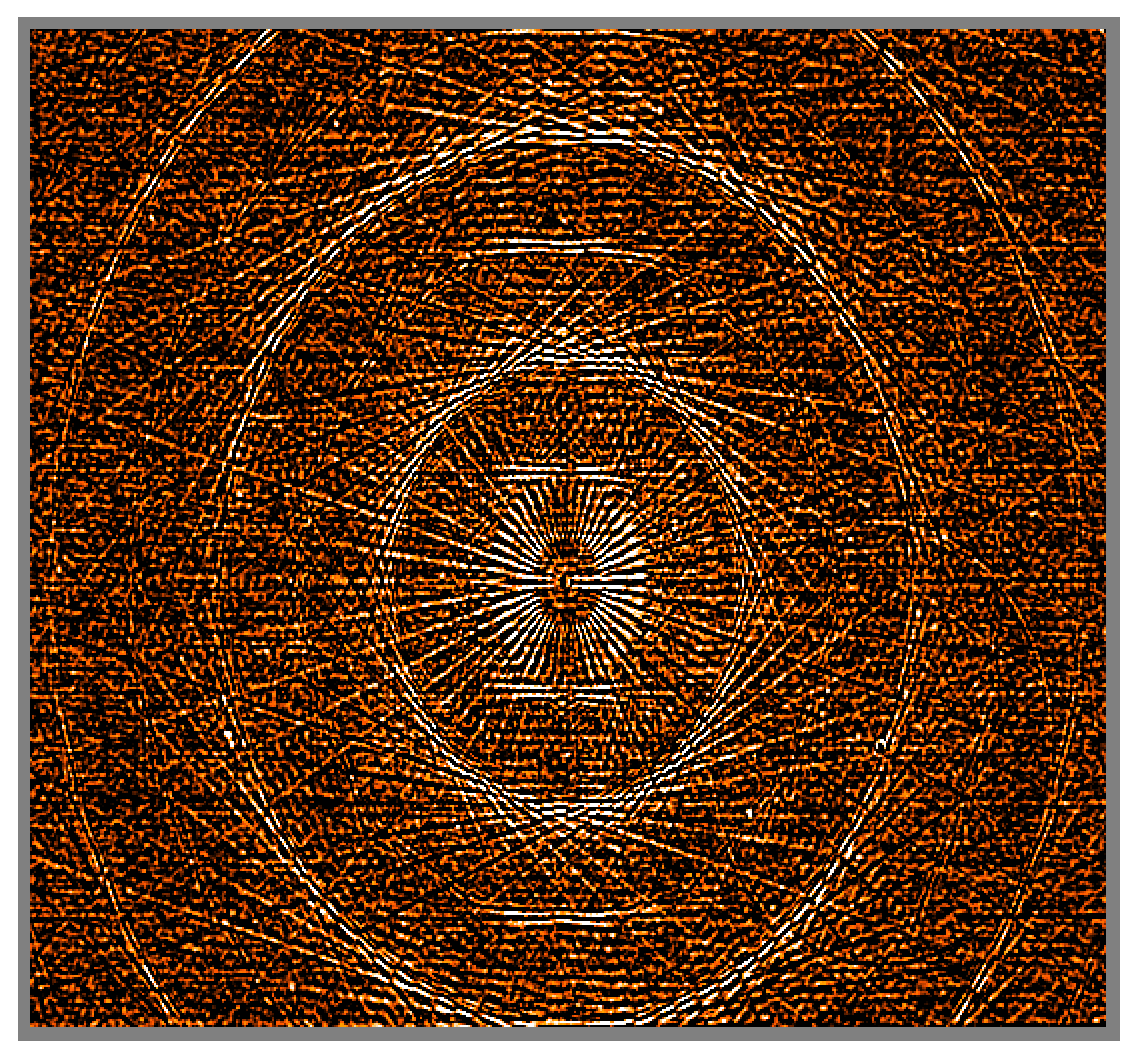
\includegraphics[width=.5\columnwidth]{B0_solution_60}%
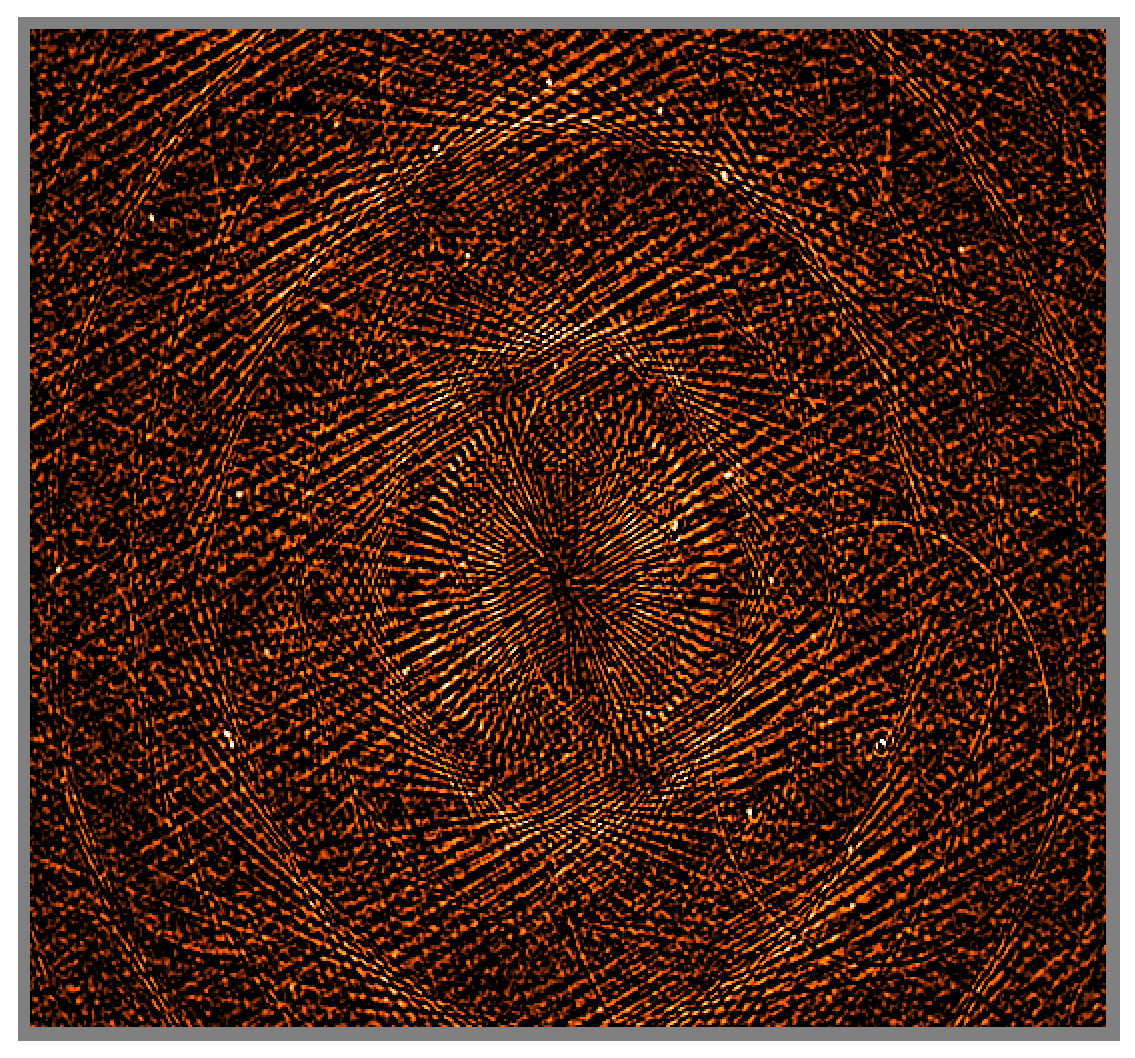
\includegraphics[width=.5\columnwidth]{B0_solution_30}\par
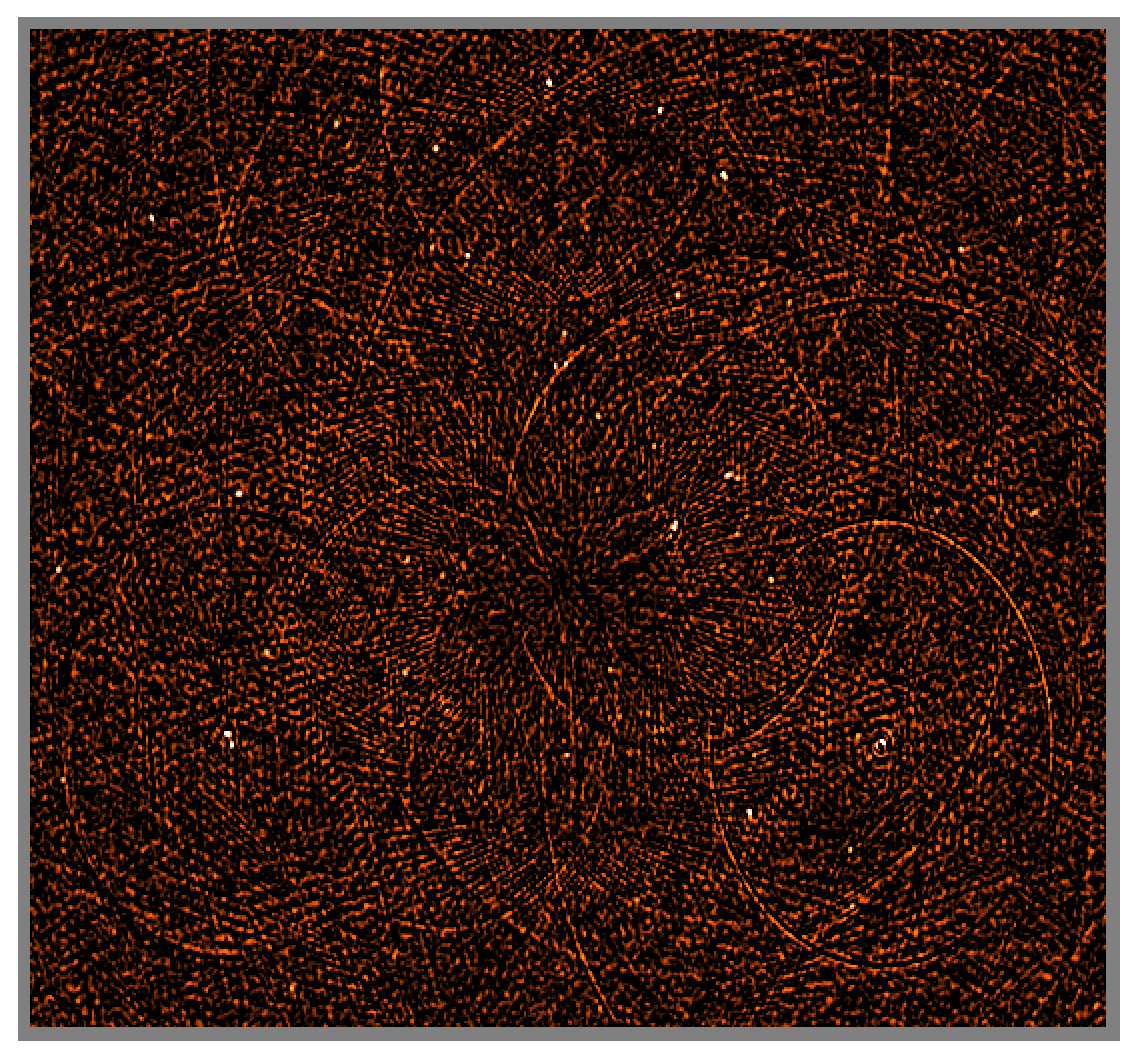
\includegraphics[width=.5\columnwidth]{B0_solution_15}%
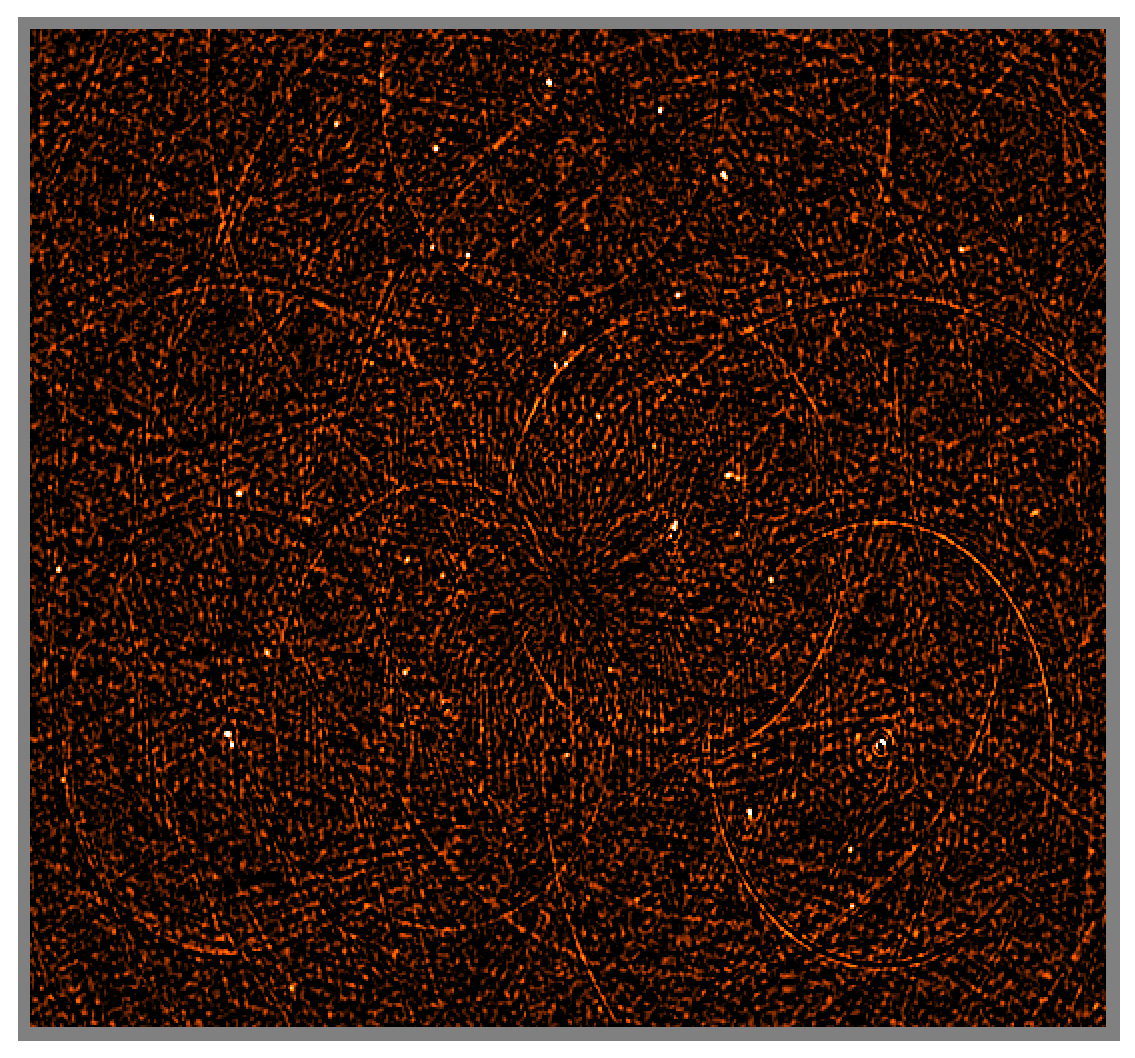
\includegraphics[width=.5\columnwidth]{B0_spline}\par
\end{centering}
\caption{\label{fig:Bsol}Single-band residual images produced via bandpass selfcal with different solution intervals for $\jones{B}{p}$: 30 minutes (upper left), 15 minutes (upper right), 7.5 minutes (lower left), and with the 7.5 minute solution smoothed using splines (lower right.) Even in the best-case image, the dominant source 3C147 was not subtracted out perfectly, leaving behind DR-limiting artifacts.}
\end{figure}

The initial result of this calibration was profoundly unsatisfactory (Fig.~\ref{fig:Bsol}, upper left). The residual image was dominated by spoke-like artifacts centered on 3C147, at about 10,000:1 level (relative the flux of 3C147 itself). These spokes correspond to edges of the 30-minute solution intervals (being an E-W array, WSRT has a one-dimensitional instantaneous PSF.) The obvious explanation for the error is short-term bandpass instability. Decreasing the solution interval of $\jones{B}{p}$ to 15 and 7.5 minutes reduced the artifacts to levels of 50,000:1 to 100,000:1, but did not eliminate them entirely. Smoothing the 7.5 minute solution with a spline (along the time axis, per each channel independently) produced a marginal improvement (Fig.~\ref{fig:Bsol}, lower right.) Subtraction artifacts are still plainly visible in the map, althought at a level not significantly above thermal noise.

At this stage we had to conclude that the WSRT bandpass exhibits some very low-level, but extremely short-term jitter, precluding a separate bandpass selfcal at extreme dynamic ranges. On the other hand, this result also shows that where a single-band dynamic range of no more than 100,000 is expected (as is the case for many other observations), bandpass selfcal provides perfectly adequate results, and can cut down on the number of solvable parameters significantly. In the meantime, for the 3C147 study we had to revert to the per-channel selfcal approach of de Bruyn.

\subsection{Per-channel selfcal}

The RIME for per-channel selfcal is just eq.~(\ref{eq:3C147:bandpass}) without the bandpass term (and is, in fact, very similar to NEWSTAR's implicit equation \ref{eq:newstar-rime}):
 
\begin{equation}\label{eq:3C147:perchan}
\coh{V}{pq} = \coh{M}{pq} \ast \left ( \jones{G}{p} \left( \sum_s E_s \coh{X}{spq} E^{\dagger}_s \right)  \jonesT{G}{q} \right )
\end{equation}

Per-channel selfcal is achieved by setting the solution interval of $\jones{G}{p}$ to one channel and one timeslot. The resulting single-band residual images are dominated by closure errors at a level of $\sim 100\mu$Jy (or 1:200,000 relative to 3C147 itself); these go away after an $\coh{M}{pq}$ solution (Fig.~\ref{fig:Gsol}). These images are qualitatively very similar to those obtained by de Bruyn during his NEWSTAR calibration (which is to be expected, given the similarity of the equations.)

\begin{figure}
\begin{centering}
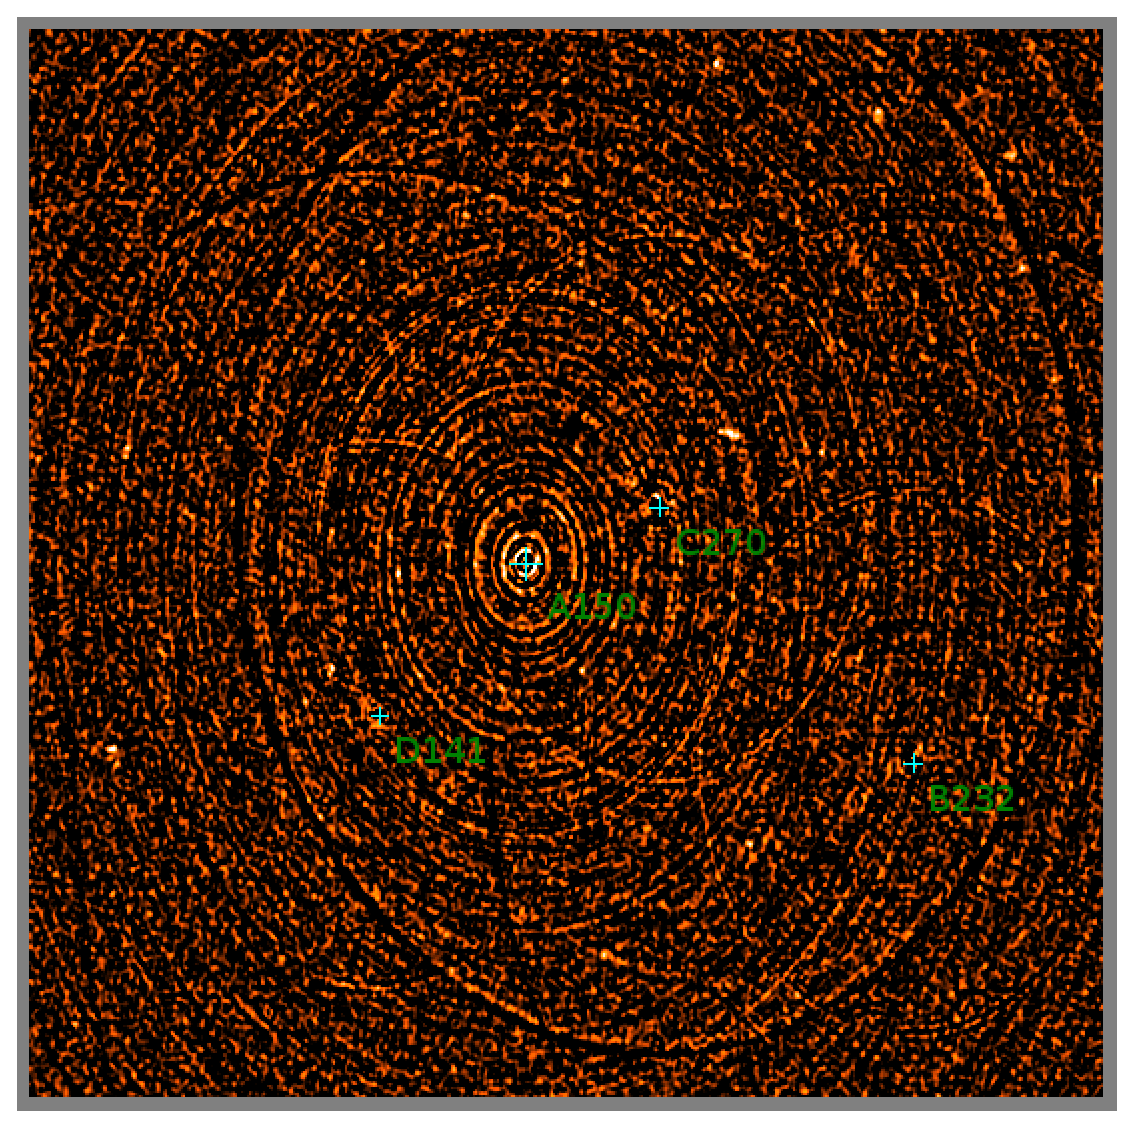
\includegraphics[width=.5\columnwidth]{G_solution}%
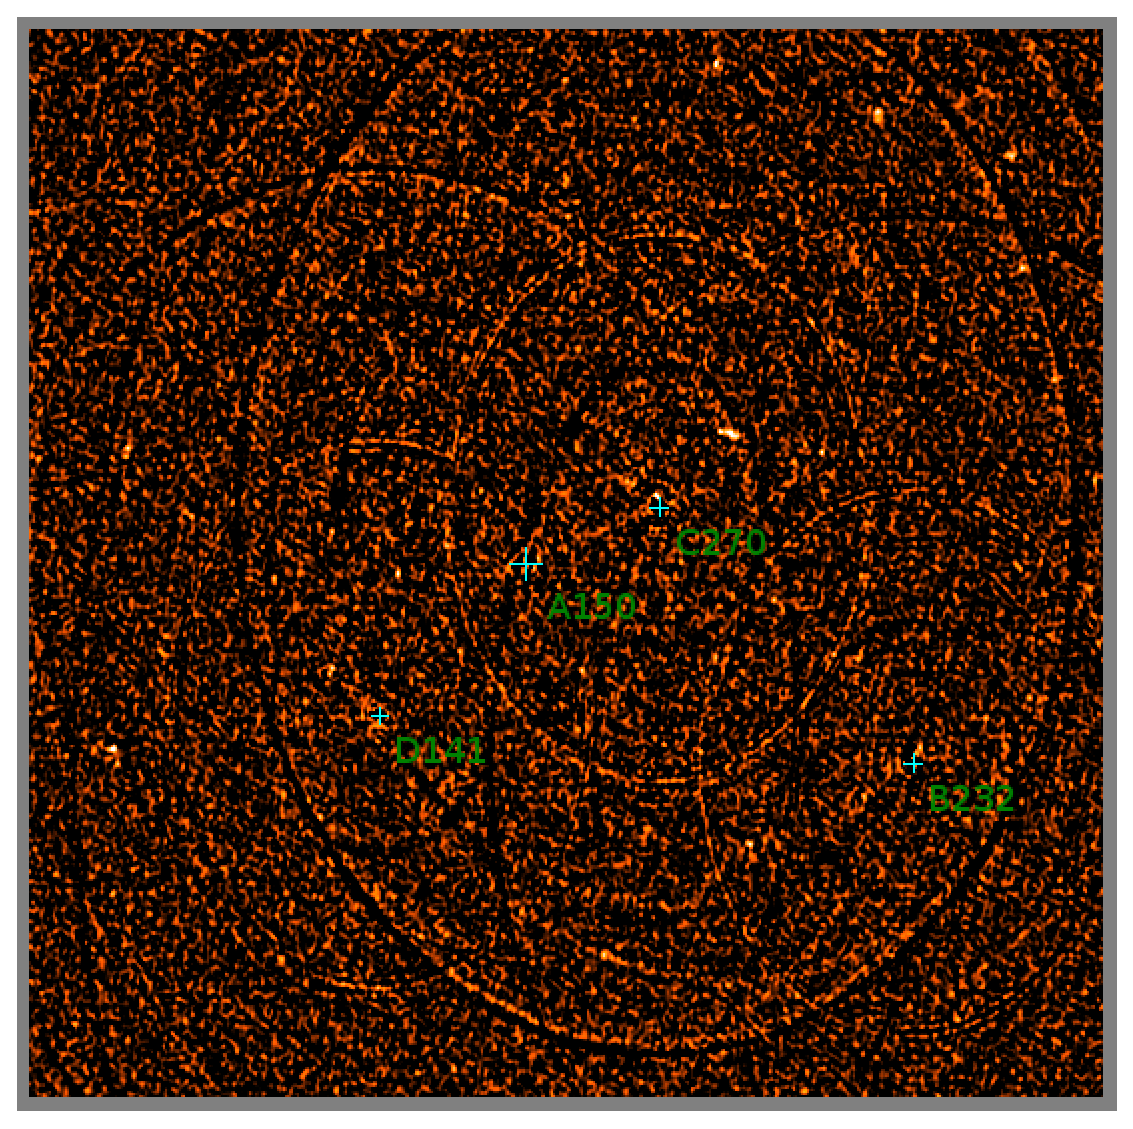
\includegraphics[width=.5\columnwidth]{IG_solution}\par
\end{centering}
\caption{\label{fig:Gsol}Single-band residual images produced via per-channel selfcal. The left image is the result of solving for $\jones{G}{p}$. It is dominated by concentric rings centered on 3C147 (designated as ``A150'' here). These are caused by closure errors, and go away once a solution for interferometer-based errors $\coh{M}{pq}$ is done (right image.) The remaining artifacts are associated with off-axis sources B, C and D, and are due to DDEs. 
}
\end{figure}

The remaining artifacts in Fig.~\ref{fig:Gsol} are associated with the three next-brightest sources\footnote{The source IDs used here follow the ``COPART'' (Clustering, Order, Position Angle, Radius, Type) convention, as implemented by the Tigger sky model management tool (available with MeqTrees.) A COPART source ID starts with an alphabetic designator (A, B, ... Z, aa, ab, ...) assigned to sources in order of decreasing brightness. This is already a unique identifier, and is sometimes used by itself for brevity, as in the paragraph above. A full ID also encodes approximate position relative to field center: two digits for the position angle (in units of $10\degr$), and one digit encodes for radial distance (in units of $10\arcmin$.) Optional suffixes incidate source type and clustering. Thus the full ID of source B is B232; being slightly extended, in this particular sky model it is actually represented by a cluster of six delta functions: B232, B232a, ... B232e.} in 
the field: B (42~mJy), C (52~mJy), and D (22~mJy). The furthest of these (B) is about 20$\arcmin$ away from centre. The artifacts themselves are within $50 \mu$Jy (thermal noise in one band is $30 \mu$Jy), or at a level of 1:1000 relative to the associated sources. This is why \citet{deBruyn:million} talks about an ``off-axis dynamic range'' of a 1000: while 3C147 itself (22~Jy) is subtracted without a trace (down to the thermal noise), the off-axis sources are only subtracted to a precision of about 1000. Some of the artifact structure is doubtlessly due to slightly under- or overestimated sky model fluxes (this produces regular rings matching the WSRT PSF), which can be taken care of during subsequent deconvolution. Most of it, however, is due to DDEs and does not deconvolve, producing artifacts in the final 8-band images such as the one shown in the left inset of Fig.~\ref{fig:3C147} (the inset is, in fact, a close-up of source B).

\subsection{Interferometer-based errors\label{sec:3C147:closure-errors}}

It is not clear what causes closure errors at the WSRT. Common sense suggests the analog part of the signal chain is to blame, but there is no hard evidence either way. What is evident is that high-DR images exhibit concentric ring-like artifacts such as those in the left image of Fig.~\ref{fig:Gsol}, and that these go away once a solution for an interferometer-based  multiplicative error -- the $\coh{M}{pq}$ term of eq.~(\ref{eq:3C147:perchan}) -- is applied. A single solution per band, per the entire 12 hours (per correlation and interferometer) is sufficient. The $\coh{M}{pq}$ solutions are usually within $10^{-3}-10^{-4}$ of unity (as is the case here), but can be much higher in some observations, for reasons that remain mysterious. 

The latter fact suggests an intrinsic time variability, but solving for $\coh{M}{pq}$ on short time intervals is very dangerous. Any solution for $\coh{M}{pq}$ will also try to compensate for observed flux that is not present in the sky model. Unless the solution interval is sufficiently long, there will be unmodelled sources with a fringe rate slow enough that their vector average visibility over the solution interval will be significantly non-zero. These sources will then tend to be attenuated by the $\coh{M}{pq}$ solutions. The 3C147 observations provide a perfect example (Fig.~\ref{fig:source-suppression}.) On the left is an 8-band residual image with a 12 hour $\coh{M}{pq}$ solution; on the right is one with a 30 minute solution. Model sources are indicated by crosses. Attenuation of unmodelled sources towards phase centre is clearly visible in the right image. 

\begin{figure}
\begin{centering}
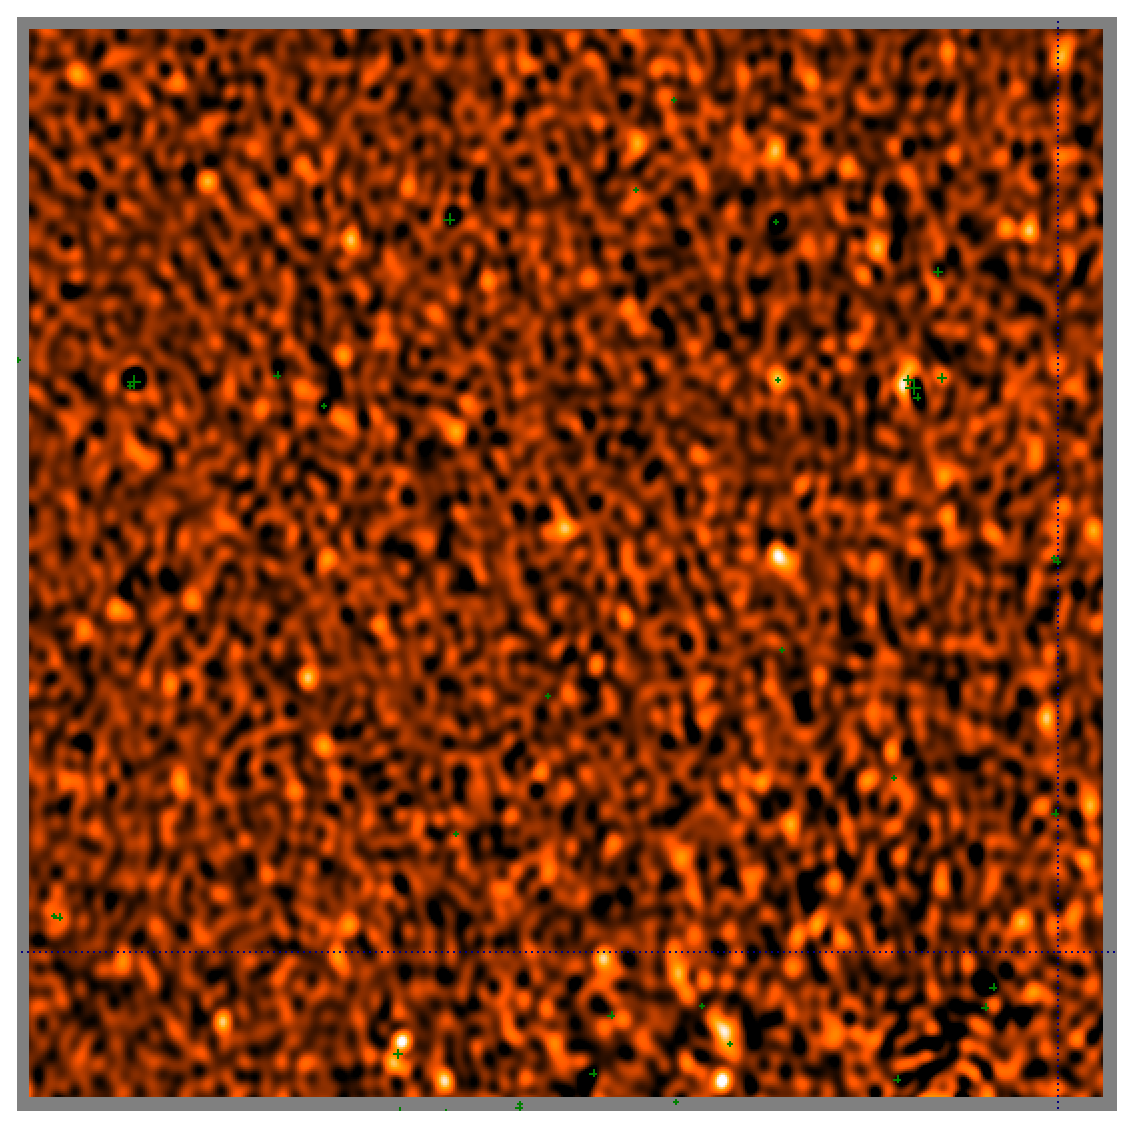
\includegraphics[width=.5\columnwidth]{IG_12h}%
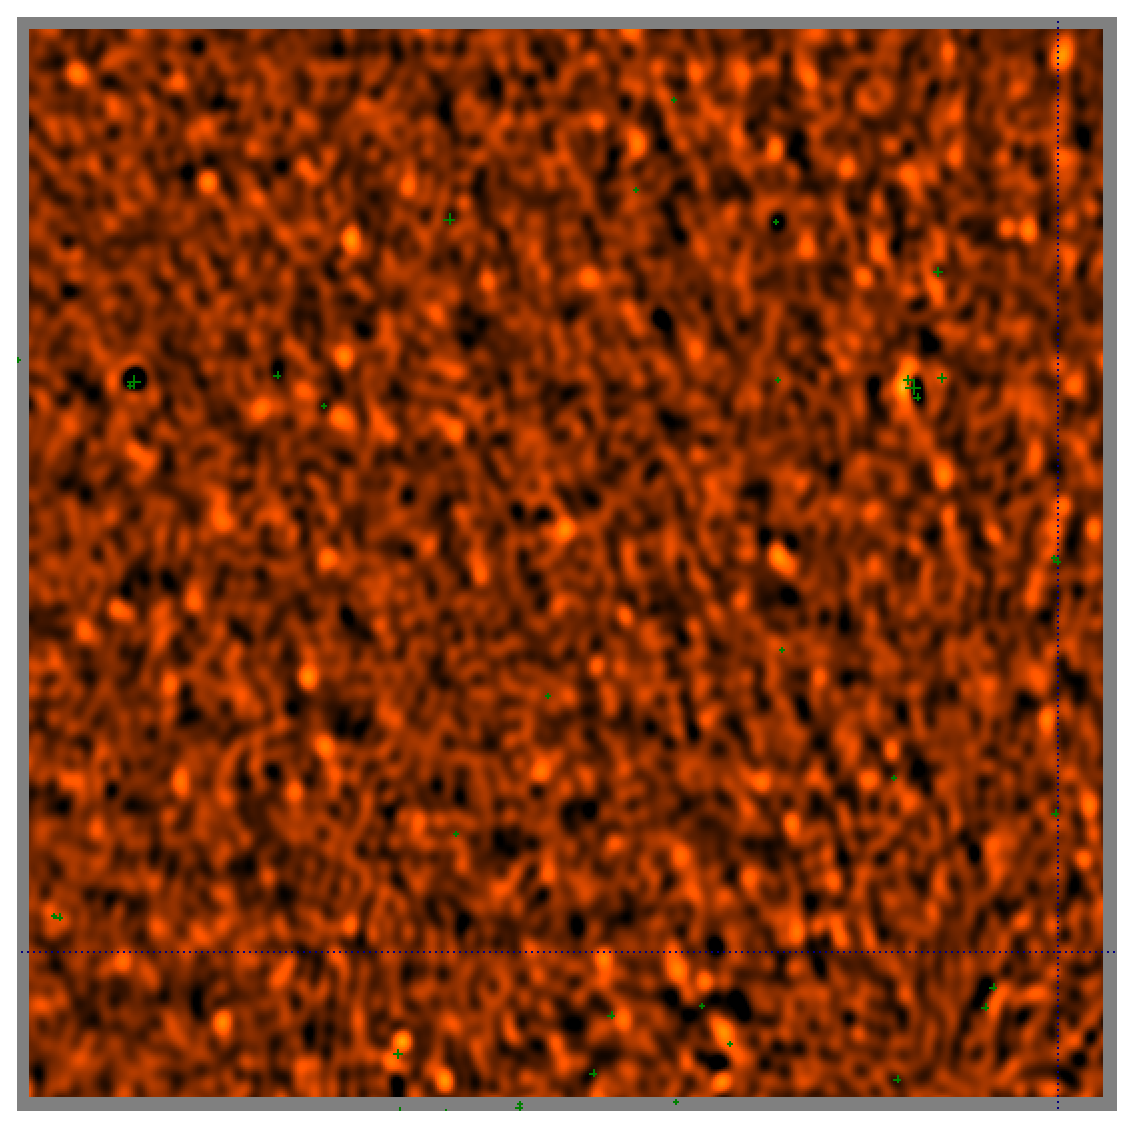
\includegraphics[width=.5\columnwidth]{IG_30m}\par
\end{centering}
\caption{\label{fig:source-suppression}Source suppression through interferometer-based error solutions. On the left is a deconvolved 8-band residual image of the center of the field, with 12 hour solutions for $\coh{M}{pq}$. On the right is the same image with 30 minute solutions. The positions of (subtracted) model sources are indicated by crosses. Suppression of unmodelled sources is evident in the right image.
}
\end{figure}


This implies that closure errors cannot be reliably solved for on observations shorter than 12 hours, unless a ``complete'' (i.e. down to the noise) sky model of the center of the field is available.

\subsection{Pointing selfcal\label{sec:3C147:pointing}}

Since the main cause of artifacts in WSRT images is commonly considered to be pointing error (see Sect.~\ref{sec:pointing}), we decided to implement a version of the pointing selfcal algorithm suggested by \citet{SB:pointing}. This proved to be a straightforward exercise in MeqTrees, since only a small modification of the RIME of eq.~(\ref{eq:3C147:perchan}) was required: 

\begin{equation}\label{eq:3C147:pointing}
\coh{V}{pq} = \coh{M}{pq} \ast \left ( \jones{G}{p} \left( \sum_s E_{sp} \coh{X}{spq} E^{\dagger}_{sq} \right) \jonesT{G}{q} \right )
\end{equation}

Instead of a per-source beam gain $E_s=E(l_s,m_s)$ (where $E(l,m)$ is the $\cos^3$ approximation given by Sect.~\ref{sec:E-Jones:wsrt}), which we had been using in the previous equations, here we used a per-antenna, per-source beam gain $E_{sp}$, defined as follows:

\begin{equation}\label{eq:3C147:offset-beam}
E_{sp} = E(l_s+\delta l_p,m_s+\delta m_p)
\end{equation}

Per-antenna pointing offsets $\delta l_p,\delta m_p$ were then treated as solvable parameters. 

The results of this proved inconclusive. Even though the solution converged to some physically-sensible offsets (on the order of arcmin), no tangible reduction of artifacts was observed in residual images. This could be due to a number of reasons:

\begin{enumerate}
\item The $\cos^3$ approximation is not good enough -- unlikely, as it has been independently verified at least for the core of the main lobe, which the sources in question sources are well within.
\item With only a few sources sufficiently bright to exhibit DDEs, we simply don't have enough constraints for a pointing solution on this field.
\item The model fluxes/positions for the sources in question are not sufficiently accurate.
\item The dominant DDE affecting this observation is not pointing error. This will be elaborated on further in Sect.~\ref{sec:de-analysis}. 
\item There is something wrong with our implementation of pointing selfcal, especially since the figures in Sect.~\ref{sec:de-analysis} suggest that mispointings \emph{are} detectable.
\end{enumerate}

Trying to get a better grip on the problem, we eventually settled on a ``controlled experiment'':
locating a field containing multiple bright off-axis sources, and observing it with deliberately exaggerated mispointings, to see if these can be more readily recovered from the data. This experiment became known as the ``QMC Project'' (in honour of the long-defunct Quality Monitoring Committee of WSRT), and was successfully carried out. The results will be presented in a follow-up paper \citep{QMC}. 
In the meantime, we had to look for alternative approaches to DDEs in the 3C147 field.

\subsection{Differential gains: the ``flyswatter''\label{sec:diffgains}}

In the spirit of ``phenomenological'' equations discussed in Sect.~\ref{sec:phenomenological}, we decided to introduce a {\em differential gain} Jones ($\Delta E$-Jones) into our form of the RIME:

\begin{equation}\label{eq:3C147:de}
\coh{V}{pq} = \coh{M}{pq} \ast \left ( \jones{G}{p} \left( \sum_s \Delta\jones{E}{sp} E_s \coh{X}{spq} E^{\dagger}_s \Delta\jonesT{E}{sq} \right)  \jonesT{G}{q} \right )
\end{equation}

The $\Delta\jones{E}{sp}$ term is meant to subsume {\bf all} DDEs associated with source $s$ and antenna $p$ (with the exception of the nominal primary beam gain, which is already represented by $E_s$). Solving for this term requires some caution, lest too many DoF's be introduced into the equation. We approached this as follows:

\begin{itemize}
\item $\Delta\jones{E}{}$ was fixed at unity for all sources except B, C, and D;
\item For B, C and D, $\Delta\jones{E}{}$ was set to a diagonal matrix with solvable complex elements.
\item The solution intervals for the $\Delta\jones{E}{}$ elements were set to one solution per 30 minutes, per entire band (and per source, antenna, receptor).
\end{itemize}

\begin{figure}
\begin{centering}
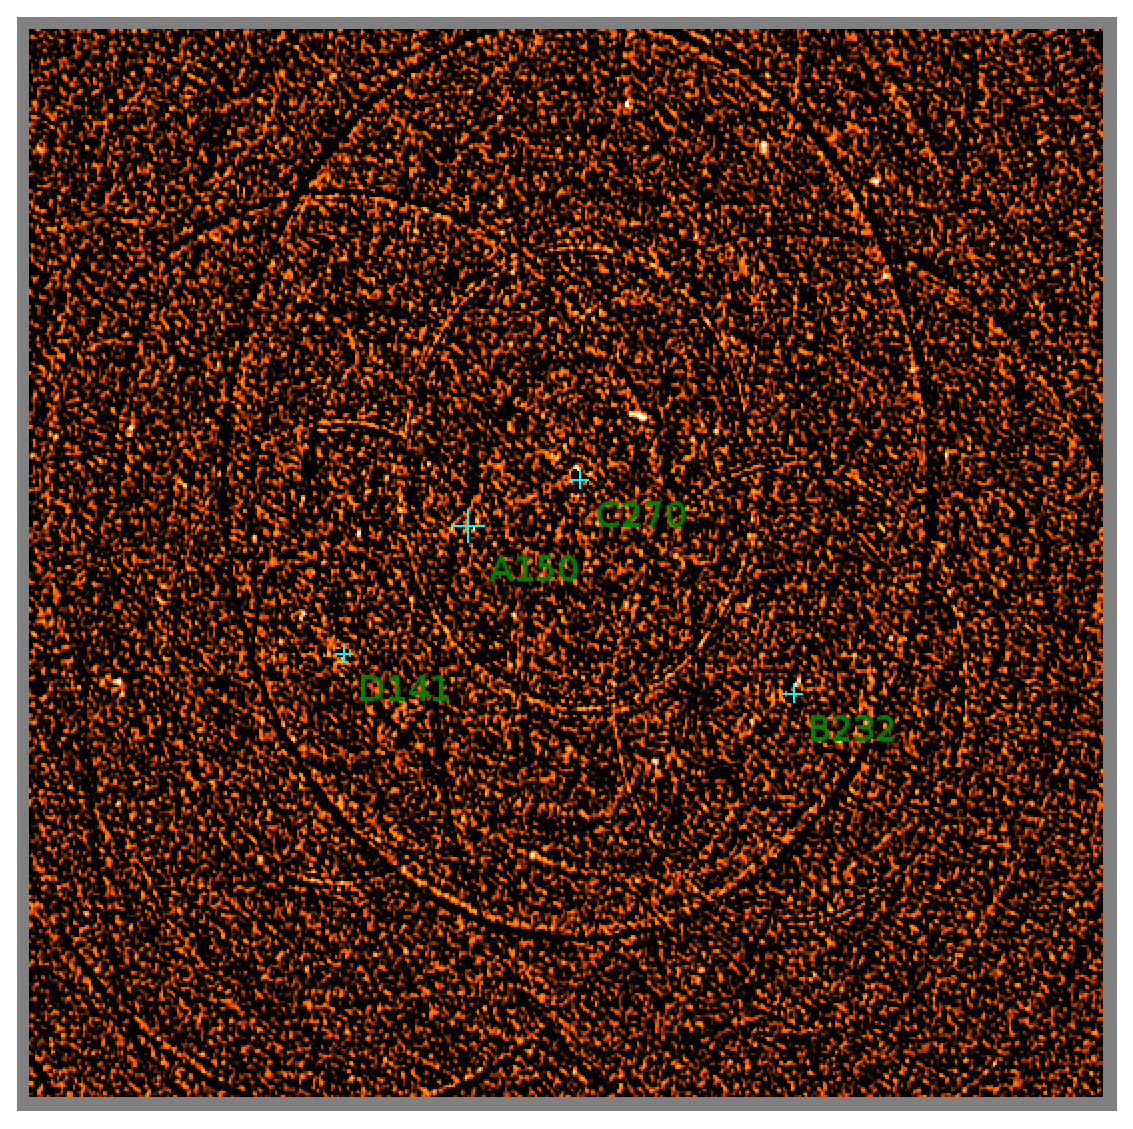
\includegraphics[width=.5\columnwidth]{before_dE}%
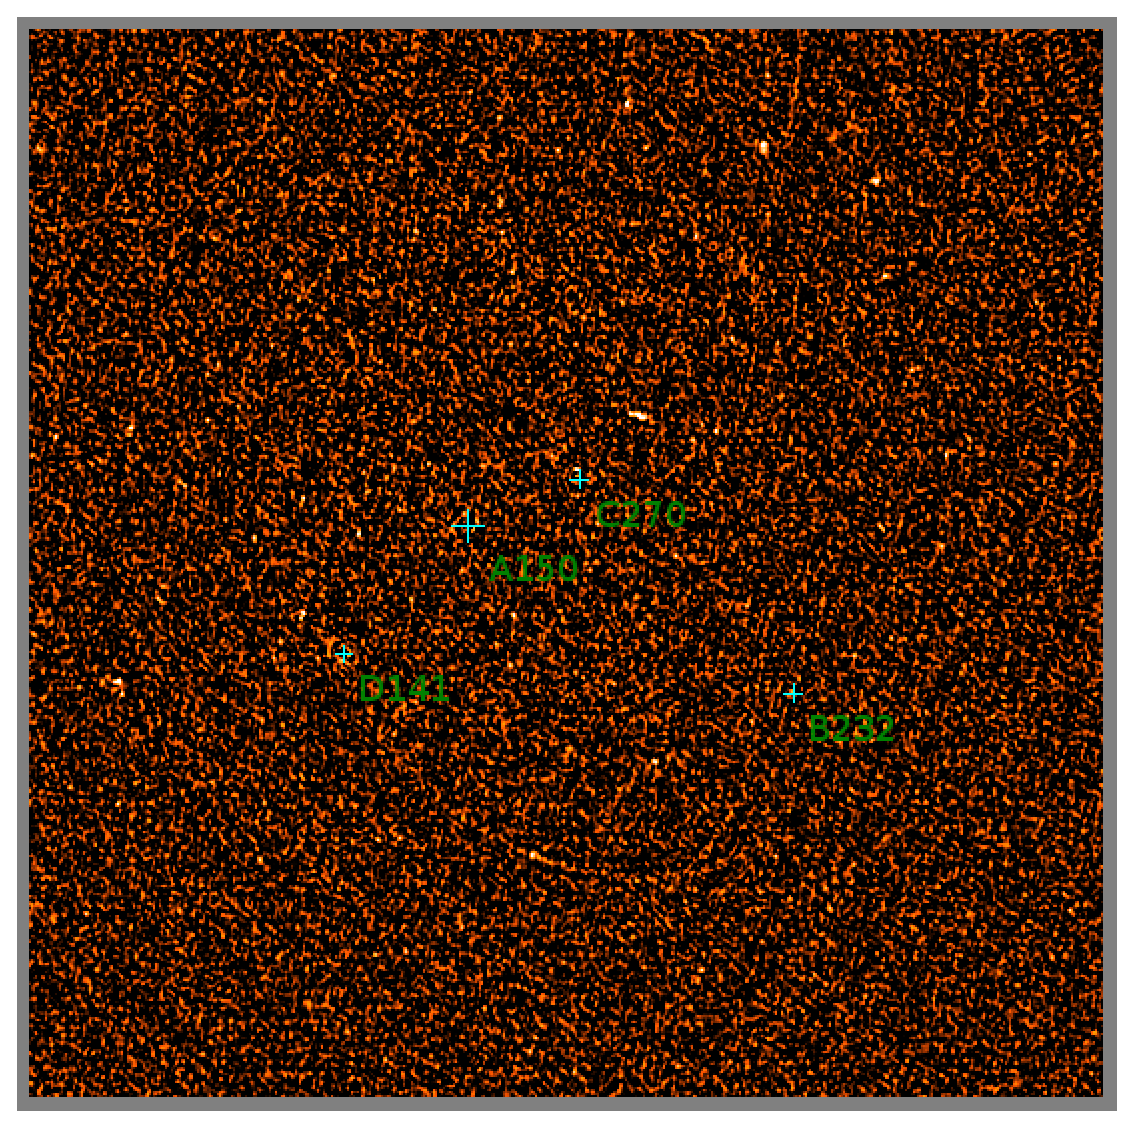
\includegraphics[width=.5\columnwidth]{after_dE}\par
\end{centering}
\caption{\label{fig:dEsol}The flyswatter. On the left is a single-band residual image after  $\jones{G}{p}$ and $\coh{M}{pq}$ solutions only. On the right is the same image with differential gain solutions for sources B, C, and D.}
\end{figure}

Figure~\ref{fig:dEsol} shows the effect of $\Delta\jones{E}{}$ solutions. All artifacts associated with sources B, C and D disappeared completely, to the point where faint artifacts around fainter sources became just about visible.  These were also eliminated once $\Delta\jones{E}{}$ solutions were enabled for those sources. In fact, any source to which a solvable $\Delta\jones{E}{}$ term was assigned promptly vanished from the residual maps, hence our name for the differential gains approach: the ``flyswatter'' algorithm. 

Once 8-band residual images were created, the increased sensitivity made it apparent that four more sources were exhibiting a small amount of DDEs. A more in-depth look at the sky model also showed that all seven sources were in fact slightly extended; the NEWSTAR model represented each by a tight cluster of point sources. Since all ``sources'' in such a cluster are subject to the same DDE, it seemed sensible to make sure the same $\Delta\jones{E}{sp}$ term was applied to all of them. This was easily done using Tigger, a sky model manager/viewer tool included with MeqTrees. Tigger automatically detects source clusters and assign source identifiers appropriately (e.g. B232, B232a, ...  B232e) It was then a simple matter to tell the Calico framework to use the \emph{same} $\Delta\jones{E}{s_0 p}$ term for all sources $s$ associated with cluster $s_0$. 

%plot-de-solutions.py --circle-ampl -o eps --portrait --borders 0.05,0.98,0.05,0.98 --title-fontsize 0 -r MS/3C*/dE* --circle-minsize=0 --circle-maxsize=0 --label-fontsize=16 --names-only --radius 70
\begin{figure}
\begin{minipage}[c]{.45\columnwidth}
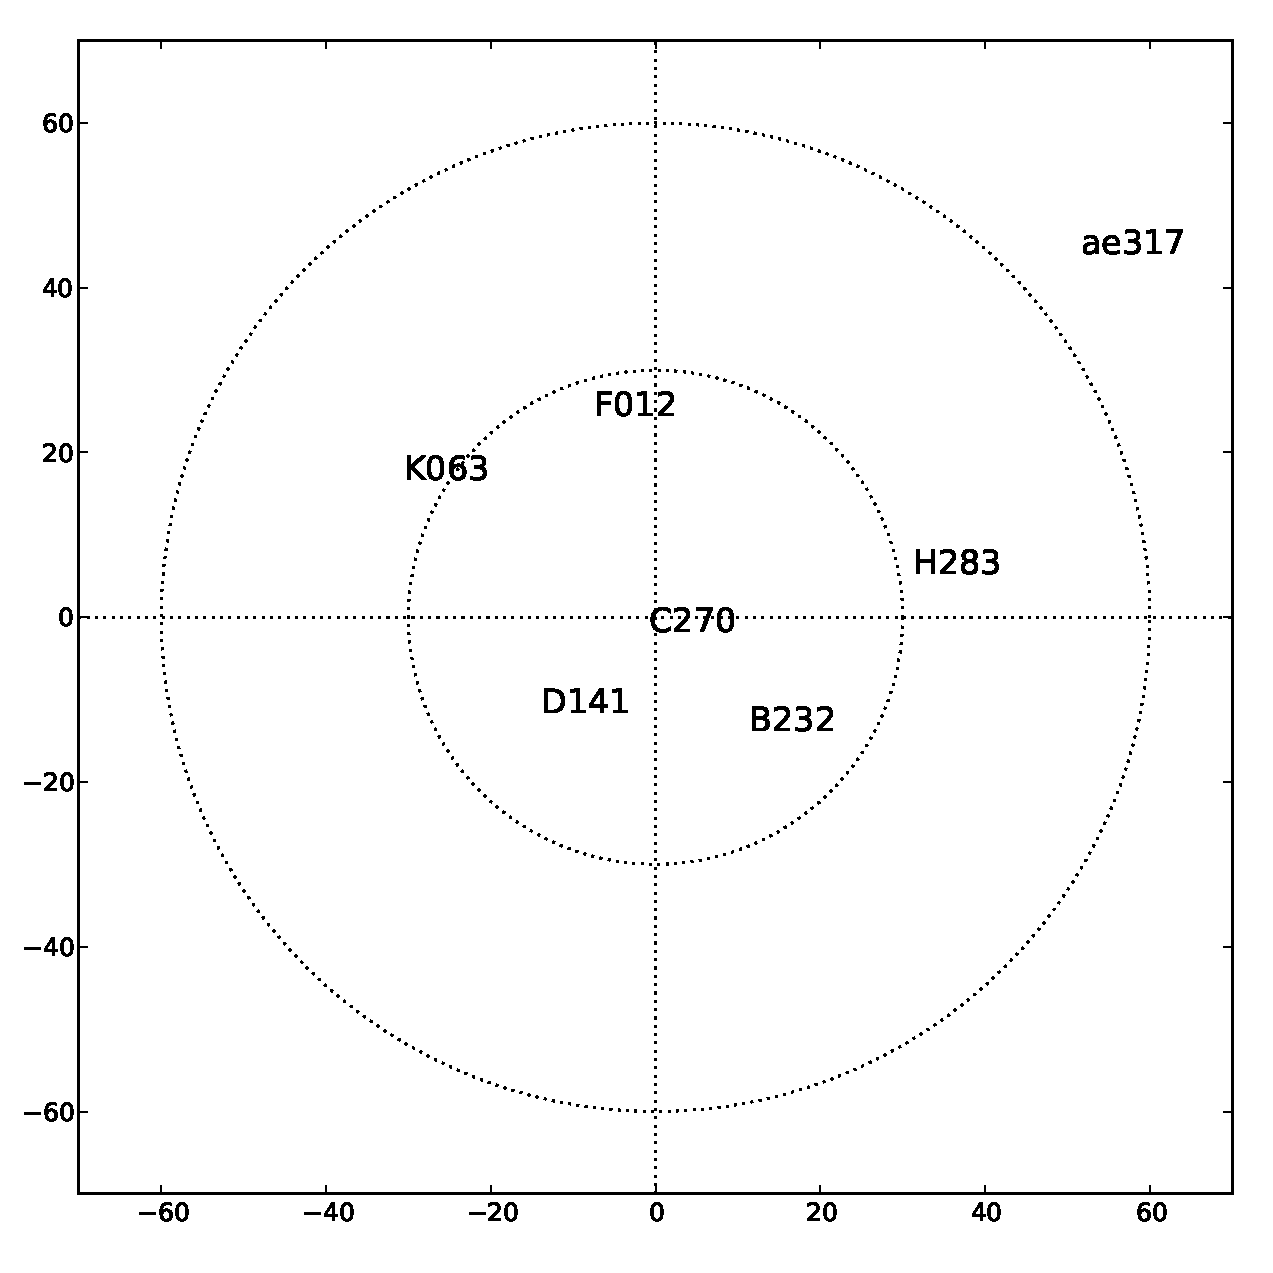
\includegraphics[width=\textwidth]{source_plot}
\end{minipage}\hfill\begin{minipage}[c]{.5\columnwidth}
\begin{tabular}{lr@{ }lr@{.}l}
\hline
\hline
ID & \multicolumn{2}{c}{position} & \multicolumn{2}{c}{total flux} \\
% \multicolumn{2}{c}{source ID} & \multicolumn{2}{c}{position} & \multicolumn{2}{c}{total flux} \\
\hline
B232  & 20' & SW & 42 & 3 mJy\\
C270  &  4' & W  & 51 & 8 mJy\\
D141  & 14' & SE & 21 & 8 mJy\\
F012  & 25' & N  & 12 & 3 mJy \\
H283  & 37' & W  &  9 & 4 mJy \\
K063  & 31' & NE &  8 & 2 mJy \\
ae317 & 74' & NW &  2 & 2 mJy \\
%  B232 & (NEWS1000)   & 20' & SW & 42 & 3 mJy\\
%  C270 & (NEWS7)      &  4' & W  & 51 & 8 mJy\\
%  D141 & (NEWS9)      & 14' & SE & 21 & 8 mJy\\
%  F012 & (NEWS1009)   & 25' & N  & 12 & 3 mJy \\
%  H283 & (NEWS1037)   & 37' & W  &  9 & 4 mJy \\
%  K063 & (NEWS1041)   & 31' & NE &  8 & 2 mJy \\
%  ae317 & (NEWS3159)  & 74' & NW &  2 & 2 mJy \\
\hline
\end{tabular}
\end{minipage}

\caption{\label{fig:source-plot}Positions (relative to nominal pointing center) and aggregate fluxes (apparent) of the seven off-axis source clusters for which $\Delta\jones{E}{}$ solutions were obtained. Circles are at  radius of $30\arcmin$ and $1\degr$. For reference, the half-maximum point of the WSRT voltage beam is $\sim25\arcmin$ at 1.4~GHz.}
\end{figure}

The seven source clusters for which differential gain solutions were eventually obtained are summarized in Fig.~\ref{fig:source-plot}. Two of them are somewhat noteworthy. Source C270 is very close to center, and therefore shouldn't be affected by DDEs as much as the other sources. It is, however, a complicated and highly polarized source, so perhaps the artifacts it exhibited after regular selfcal were primarily due to sky model inaccuracies, which the $\Delta\jones{E}{}$ solutions absorbed (see discussion in Sect.~\ref{sec:de-analysis-model}). Source ae317 is almost the opposite: it is very faint, but far enough off-axis to be in a sidelobe of the primary beam, and so subject to especially severe DDEs.

We should note that the differential gains approach is closely related to the peeling algorithm (Sect.~\ref{sec:peeling}). It can be considered a form of ``simultaneous'' peeling. In fact, solving for $\Delta\jones{E}{}$ on a single off-axis source is equivalent to peeling that source (with suitable solution intervals chosen for the selfcal step.) The $\Delta\jones{E}{}$ approach overcomes a lot of the drawbacks of peeling (cross-contamination of solutions, the need for repeated selfcal cycles) by doing a single simultaneous solution in one step.


\subsection{The showcase result} 

The ultimate result of our calibration of the 2003 observation is shown in Fig.~\ref{fig:3C147}. This image is a true showcase for the differential gains approach. The precise steps leading to this image were as follows:

\begin{enumerate}

\item Each of the 8 bands was independently calibrated using per-channel selfcal, interferometer-based errors, and $\Delta\jones{E}{}$ solutions on seven source clusters, as described above. Corrected residuals were generated.

\item The residuals for all 8 bands were imaged together (in MFS mode) to produce a single residual image. This revealed a large number of fainter sources not visible in the per-band maps.

\item The 8-band image was deconvolved using Cotton-Schwab CLEAN \citep{Schwab:csclean}.

\item The sky model was added back into the deconvolved image, using a Gaussian restoring beam.

\end{enumerate}

The resulting image is completely artifact-free. Presumably, all other sources in the field were too faint to exhibit any DDE-related artifacts. With a dynamic range of 1,600,000:1, this image is the deepest and cleanest single-synthesis radio map in the world to date. 

\subsection{Flyswatter limitations}

While it can help produce spectacular images, the flyswatter has some serious caveats and drawbacks that need to be explored. First of all, it is a brute force approach, in the sense that it squashes all effects into a single $\Delta\jones{E}{}$ term. This includes inaccuracies in the sky model! Indeed, any missing source flux or error in source position can be accomodated with a suitable $\Delta\jones{E}{}$. Even unmodelled source structure can ``leak'' into differential gain solutions (Sect.~\ref{sec:de-analysis-model}). Thus, differential gains are good for subtracting sources, but at the cost of mashing up information on the source per se. (One does not use a flyswatter to probe a fly's anatomy!)

Secondly, solvable differential gains can lead to a proliferation of DoF's. Per-channel selfcal has $N_\mathrm{ant}$ unknowns per $N_\mathrm{ant}(N_\mathrm{ant}-1)/2$ measurements, or $2/(N_\mathrm{ant}-1)$ unknowns per measurement; differential gains add $2N_\mathrm{src}/(N_\mathrm{ant}-1)N_\mathrm{time}N_\mathrm{freq}$ unknowns per measurement, where $N_\mathrm{time}$ and $N_\mathrm{freq}$ are the sizes of the solution interval for $\Delta\jones{E}{}$. This ratio remains facourable for small $N_\mathrm{src}$ and large $N_\mathrm{time}$ and/or $N_\mathrm{freq}$ (as is the case for our 3C147 reduction), but one must be careful.

The third caveat is processing cost. While usually not as expensive in terms of I/O or CPU as peeling (which, in addition to the solutions themselves, requires repeated subtraction and phase shifting steps), the flyswatter is not free. Every source with a differential gain solution adds $4N_\mathrm{ant}$ unknowns (assuming a diagonal complex $\Delta\jones{E}{sp}$ term, hence 4 real values per matrix) to the equations. As the number of unknowns ($N_\mathrm{unk}$) grows, inversion of the normal matrix within the least-squares solver becomes a CPU bottleneck, since it scales as $O(N_\mathrm{unk}^3)$. This makes it impractical to solve for $\Delta\jones{E}{}$'s for more than a handful\footnote{The precise meaning of a ``handful'' here depends on additional factors such as $N_\mathrm{ant}$, size of solution intervals, etc. In effect, these factors influence the constant of the overall cubic scaling law.} of sources at a time. 

One way to mitigate the solver bottleneck is to decompose the $\Delta\jones{E}{sp}$'s into nearly-orthogonal sets of unknowns. For example, we can treat the set of $\Delta\jones{E}{sp}$'s associated with one source $s$ as independent from all other sources. The $(4N_\mathrm{ant}N_\mathrm{src})^2$ normal matrix inside the solver then becomes block-diagonal, composed of $N_\mathrm{src}$ blocks of size $(4N_\mathrm{ant})^2$. Inversion of such a matrix then scales only linearly with the number of sources. The trade-off is slower convergence, requiring more iterations. For large numbers of sources this trade-off is extremely favourable.

\subsection{Analysis of differential gain solutions\label{sec:de-analysis}}

It is time to see whether any useful information can be gleaned from the differential gains solutions themselves. As a result of the reduction, we had obtained: per each source direction (7 of these: see Fig.~\ref{fig:source-plot}), per each antenna (14), per each band (8), per 30-minute interval (24 of these in a 12-hour synthesis), two complex numbers representing the apparent differential gain of the X and Y dipole (``differential'' being relative to the gain in the direction of 3C147 -- almost at the center of the field -- which had been taken care of by regular selfcal.)

We then adopted the following approach. Given the relatively low fractional bandwidth, we didn't expect much variation with frequency in $\Delta\jones{E}{}$. We therefore treated each set of 8 per-band solutions as independent samples of the same variable. The mean of the 8 samples was used as an estimator of variable, and the standard deviation of the 8 samples as an estimator of the error (i.e. the error bar.)

Since it quickly became apparent that the $\Delta\jones{E}{}$ solutions were exhibiting some very interesting behaviour, we applied exactly the same procedure to the 2006 observations, so that comparisons could be made. The plots below show the results from both observations. 

% plot-de-solutions.py --ampl --phase -o eps -r --portrait --title-fontsize 0 -W 290 -H 100 --borders 0.02,1.02,0.01,1.08 MS/3C*/dE* --output-prefix o2003 -c o2003
% plot-de-solutions.py --ampl --phase -o eps -r --portrait --title-fontsize 0 -W 290 -H 100 --borders 0.02,1.02,0.01,1.08 MS/m30*/dE* --output-prefix o2006 -c o2006
\begin{figure*}
\sidecaption
\parbox[b]{12cm}{
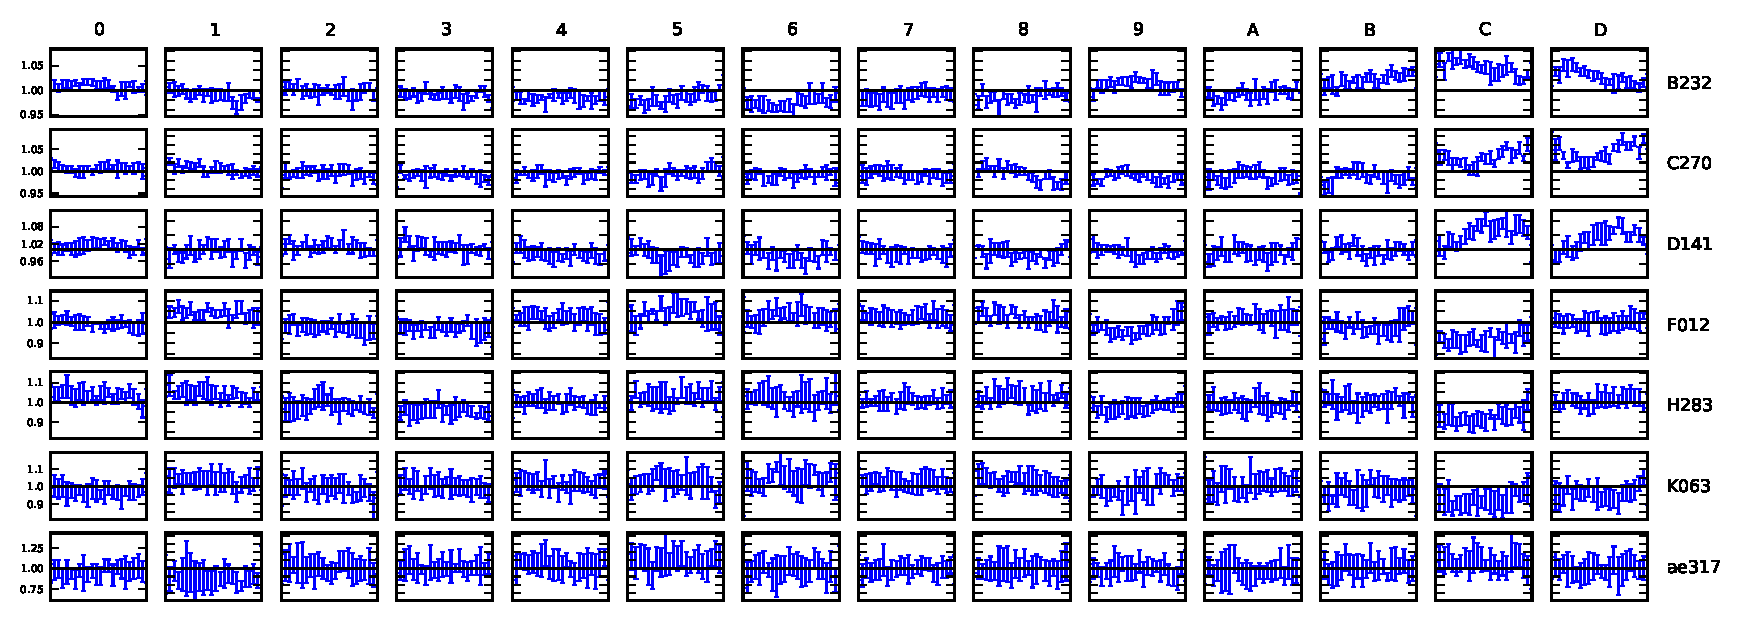
\includegraphics[width=12cm]{o2003_dE_mean} \\
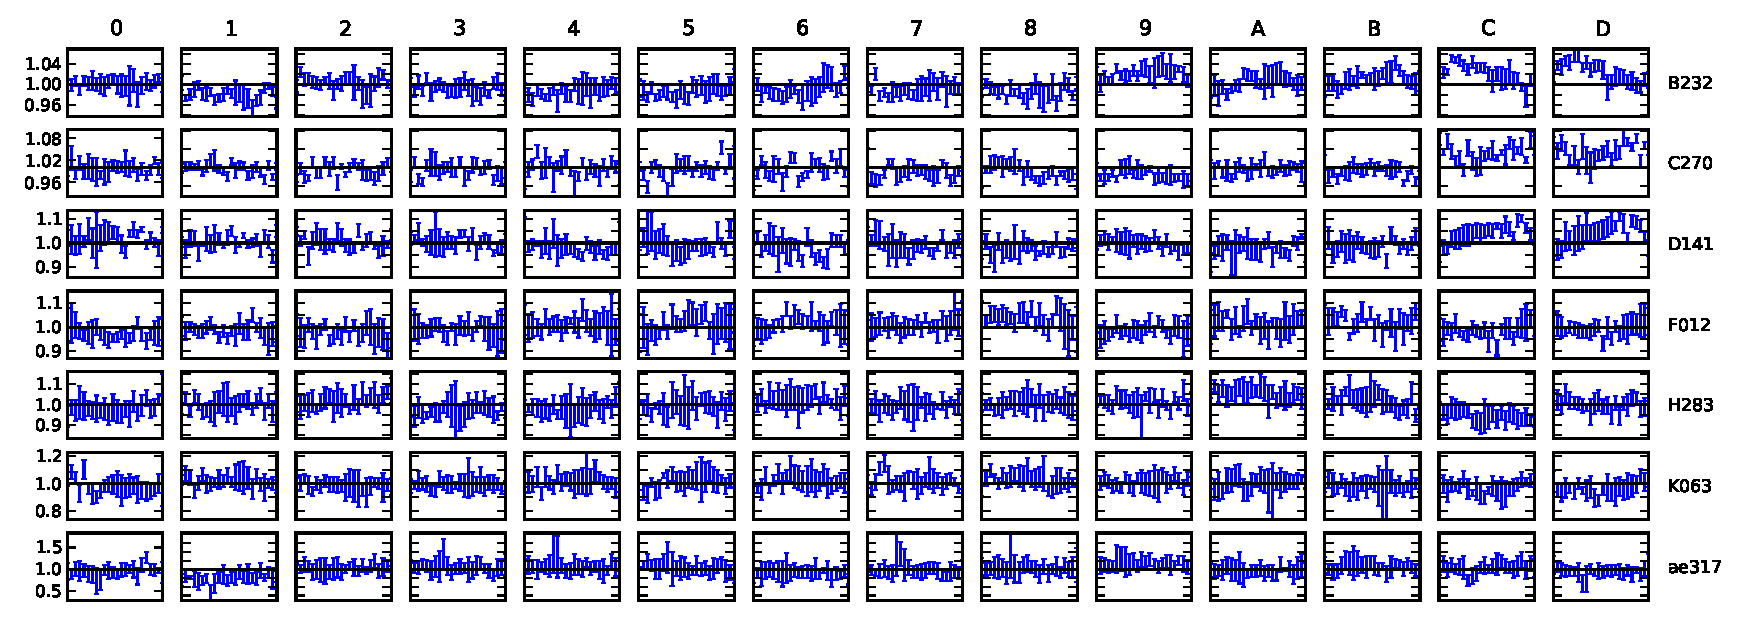
\includegraphics[width=12cm]{o2006_dE_mean}
}
\caption{\label{fig:dEampl}Differential gain-amplitudes ($||\Delta\jones{E}{}||$) as a function of time for the 2003 (top) and 2006 (bottom) observations. Rows correspond to sources, columns to antennas. The vertical plot scale is fixed within each row, but differs from row to row. Horizontal lines indicate the $||\Delta\jones{E}{}||=1$ level.}
\end{figure*}

\begin{figure*}
\sidecaption
\parbox[b]{12cm}{
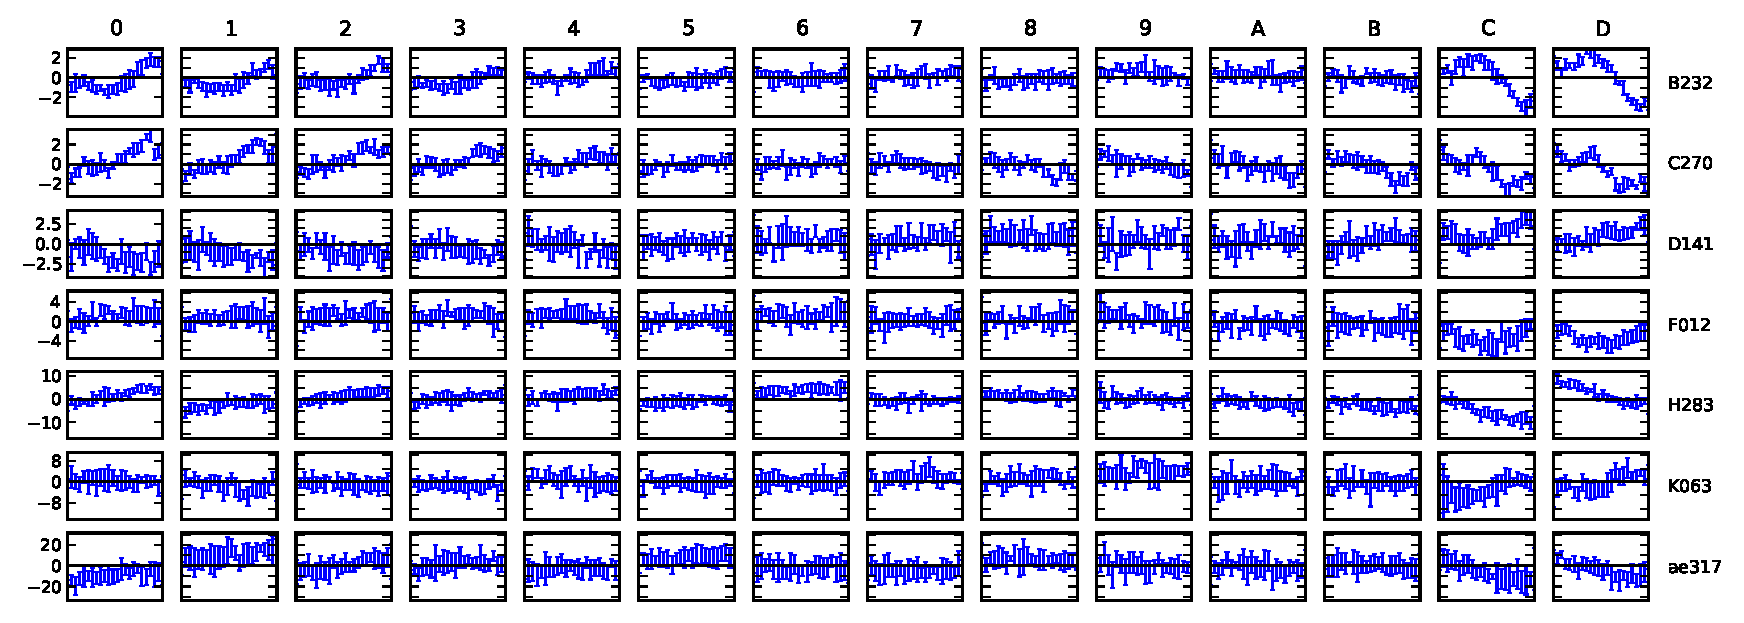
\includegraphics[width=12cm]{o2003_dEphase_mean}
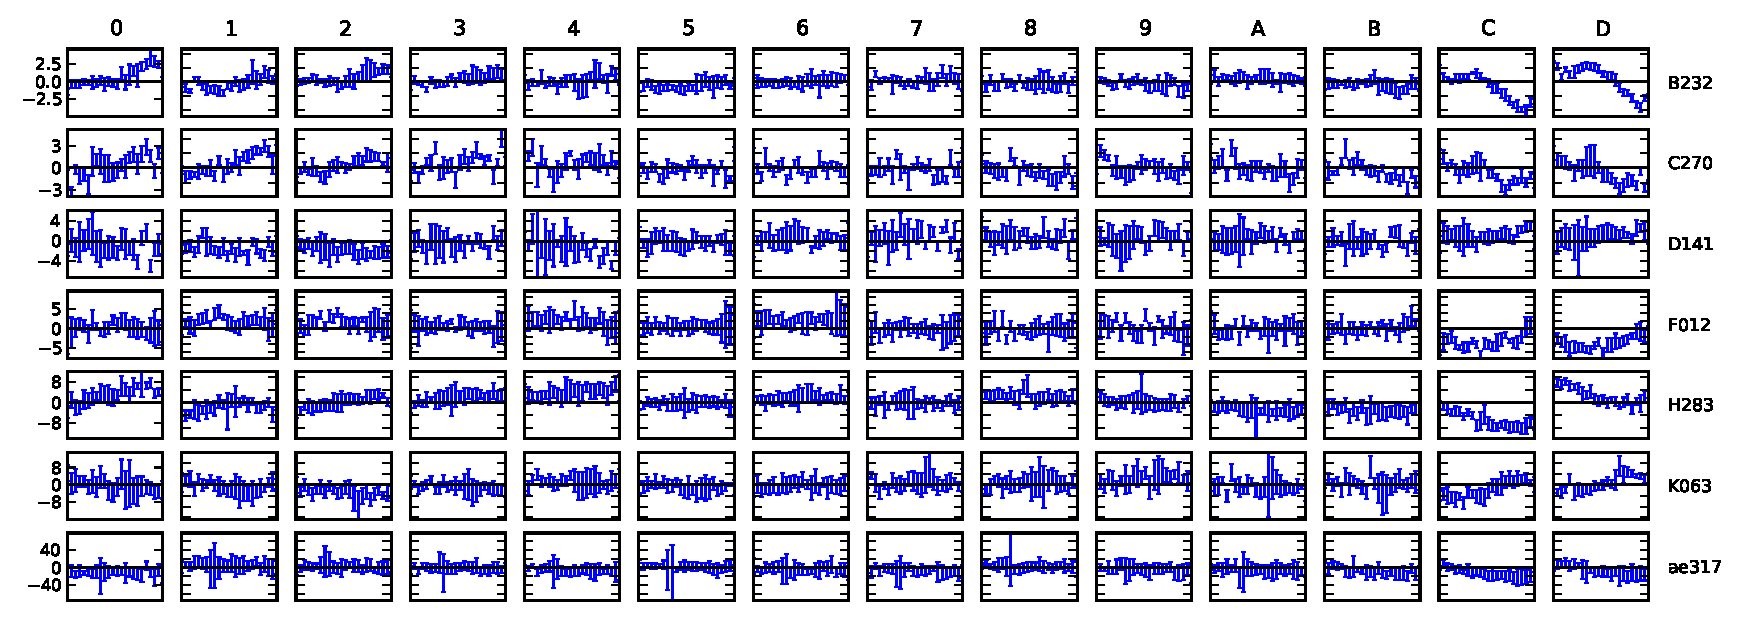
\includegraphics[width=12cm]{o2006_dEphase_mean}
}
\caption{\label{fig:dEphase}Differential gain-phases ($\arg\Delta\jones{E}{}$, in degrees) as a function of time for the 2003 (top) and 2006 (bottom) observations. Rows correspond to sources, columns to antennas. The vertical plot scale is fixed within each row, but differs from row to row. Horizontal lines indicate the $\arg\Delta\jones{E}{}=0$ level.}
\end{figure*}

Figure~\ref{fig:dEampl} is a summary of the differential gain-amplitudes per source, per antenna. The precise quantity plotted here was computed as follows. First, we computed the norm of the $\Delta\jones{E}{}$ matrix (diagonal by construction) as 

\[
\left|\left|\matrixtt{a}{0}{0}{b}\right|\right| \equiv \sqrt{|a|+|b|},
\]

i.e. as the geometric mean of the X and Y gain-amplitudes. We then normalized (divided) this value by the mean value per source (that is, the mean across all time intervals, bands, and antennas), which was meant to take out the effect of incorrect model fluxes (see below.) The resulting ``normalized norm'' was then plotted as a function of time, per source, per antenna.

Figure~\ref{fig:dEphase} is a similar plot of the differential gain-phases, computed as

\[
\arg\matrixtt{a}{0}{0}{b} \equiv \frac{\arg a + \arg b}{2}.
\]

The most striking feature of Figs.~\ref{fig:dEampl} and \ref{fig:dEphase} is the high SNR. They show a high degree of temporal continuity in the solutions, and statistically significant structure. This strongly suggests that the solutions represent real physical or numerical effects. As to the nature of these effects, we still do not have satisfactory answers, though it is hoped that the QMC project \citep{QMC} mentioned earlier will shed some more light on the issues. The rest of this section discusses some of the more prominent questions, and proposes some rather speculative explanations.
 
\subsubsection{Absorbing errors in the sky model\label{sec:de-analysis-model}}

As already mentioned, a major caveat of the flyswatter approach is that $\Delta\jones{E}{}$ solutions will tend to absorb inaccuracies in the source model. By analogy (and for exactly the same reasons), classic selfcal 
alone cannot solve for absolute positions or fluxes. Indeed, if the true position of a source $\vec l = (l,m)$ is offset from the model position $\vec l^\mathrm{(mod)} = (l+\delta l,m + \delta m)$, while the true brightness $\coh{B}{}$ differs from the model brightness by a multiplicative matrix factor: $\coh{B}{}^\mathrm{(mod)} = \jones{A}{} \coh{B}{} \jonesT{A}{}$ (the latter being a straightforward generalization of a scalar factor $a^2$), then the coherency term of the RIME for the model source may be written out as

\begin{eqnarray*}
\coh{X}{pq}^\mathrm{(mod)} & = & K_{p}(l+\delta l,m+\delta m) \coh{B}{}^\mathrm{(mod)} K^\dagger_{q}(l+\delta l,m+\delta m) \\
 & = & K_{p}(\delta l,\delta m) K_{p}(l,m) \jones{A}{}\coh{B}{}\jonesT{A}{} K^\dagger_{q}(l,m) K^\dagger_{q}(\delta l,\delta m) \\
 & = & (K_{p}(\delta l,\delta m)\jones{A}{})(K_{p}(l,m)\coh{B}{}K^\dagger_{q}(l,m))(K_{q}(\delta l,\delta m)\jones{A}{})^\dagger \\
 & = & (K_{p}(\delta l,\delta m)\jones{A}{}) 
       \cdot \coh{X}{pq} \cdot 
       (K_{q}(\delta l,\delta m)\jones{A}{})^\dagger.
\end{eqnarray*}

If a solvable differential gain is then assigned to the source, the model can be made to fit the data by absorbing the $K_{p}(\delta l,\delta m)\jones{A}{}$ factor into the $\Delta\jones{E}{ps}$ solutions.

Even more insidiously, differential gains can absorb some source structure. Consider a source that is slightly extended in one direction, enough to be resolved on the longest baselines. An E-W array like the WSRT has a one-dimensional instantaneous {\em fan beam}. It will ``see'' the source as a point source when the fan beam is aligned with the source orientation, and start resolving it when the fan beam becomes perpendicular to the source. In other words, the apparent flux of the source will remain constant in time on short baselines, and vary in time on the long baselines as the source resolves. If such a source is represented by a point source in the sky model, the model flux will be constant on all baselines. Now, if some antennas are predominantly involved in long baselines (RTC and RTD, in the case of WSRT), $\Delta\jones{E}{}$ solutions can compensate for some of the flux discrepancy by changing the gain-amplitudes of these antennas. We would expect to see a variation of $||\Delta\jones{E}{}||$ with a 12-hour period. Since most of the baselines to RTC and RTD are mutually redundant (0-C equals 1-D, etc.), their variation in $||\Delta\jones{E}{}||$ should be very similar. 

This is exactly what we're seeing in Fig.~\ref{fig:dEampl}! The plots very strongly suggest that the top three sources (B, C and D) are indeed slightly resolved. If this is the case, then the dominant contribution to $||\Delta\jones{E}{}||$ on antennas RTC and RTD is due to source structure rather than any actual DDE. 

\subsubsection{Amplitude behaviour}

If the behaviour of differential amplitude on RTC and RTD is due to source structure, this still leaves effects on the other antennas unexplained. First let us consider what a pointing error would look like. With the exception of source ae317 (for which the solutions are much too noisy anyway), the other six sources are well within the main lobe of the primary beam, where the beam gain can be expected to decrease smoothly with distance from pointing center. We should therefore expect to see $||\Delta\jones{E}{sp}||>1$ if antenna $p$ mispoints \emph{towards} source $s$ (the source appears brighter on antenna $p$), and $||\Delta\jones{E}{sp}||<1$ if it mispoints \emph{away}. WSRT dishes are equatorially mounted, so mispointings due to mechanical or electronic errors in either axis drive would be stationary with respect to the sky, and thus cause constant 
$||\Delta\jones{E}{}||$ offsets. Mispointings due to wind pressure, thermal or gravitational deformation, on the other hand, would be intrinsically time-variable (but would probably correlate between antennas.)

Quite a few plots in Fig.~\ref{fig:dEampl} do show (mostly) static offsets. It can be illuminating to present $||\Delta\jones{E}{}||$ in a format we call the ``rogues gallery'' (Figs.~\ref{fig:rogues-2003} and \ref{fig:rogues-2006}). This shows, for each of the 14 antennas, a 12-hour average $||\Delta\jones{E}{}||$ per source, using circles of varying size placed at the position of the source. The magnitude of $(||\Delta\jones{E}{}||-1)$ is indicated by circle size, and the sign by colour. A static mispointing in, e.g., a Northern direction would show up as blue circles in the top half of the plot (i.e. sources appearing brighter), and red circles in the bottom half.

\newlength{\roguewidth}
%\setlength{\roguewidth}{2.4cm} % for 12 cm figure
%\setlength{\roguewidth}{3.4cm} % for double-column figure
\setlength{\roguewidth}{.2\columnwidth} % for single-column figure

%plot-de-solutions.py --circle-ampl -o eps --portrait --radius 40 --circle-borders 0.05,0.98,0.05,0.9 --title-fontsize 40 -r o2003.cache --circle-minsize=0 --circle-maxsize=200 --label-fontsize=0 --output-prefix o2003
%plot-de-solutions.py --circle-ampl -o eps --portrait --radius 40 --circle-borders 0.05,0.98,0.05,0.9 --title-fontsize 40 -r o2006.cache --circle-minsize=0 --circle-maxsize=200 --label-fontsize=0 --output-prefix o2006

\begin{figure}
\centering
\begin{tabular}{@{}c@{}c@{}c@{}c@{}c@{}}
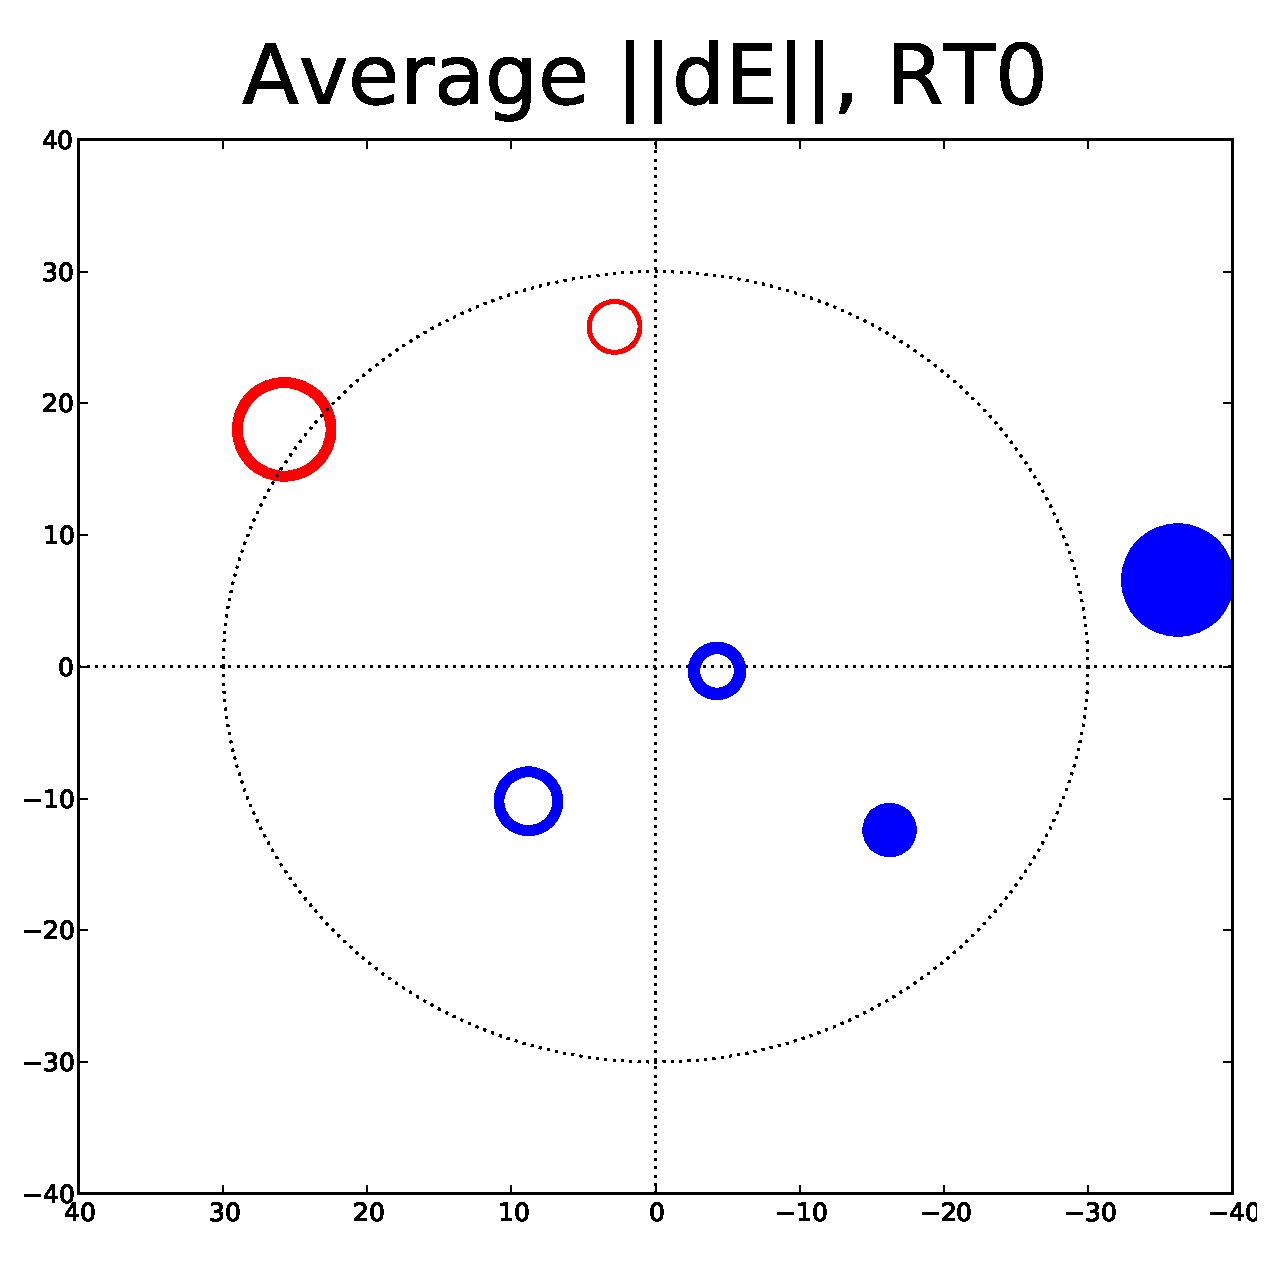
\includegraphics[width=\roguewidth]{o2003_dE_ant0} &
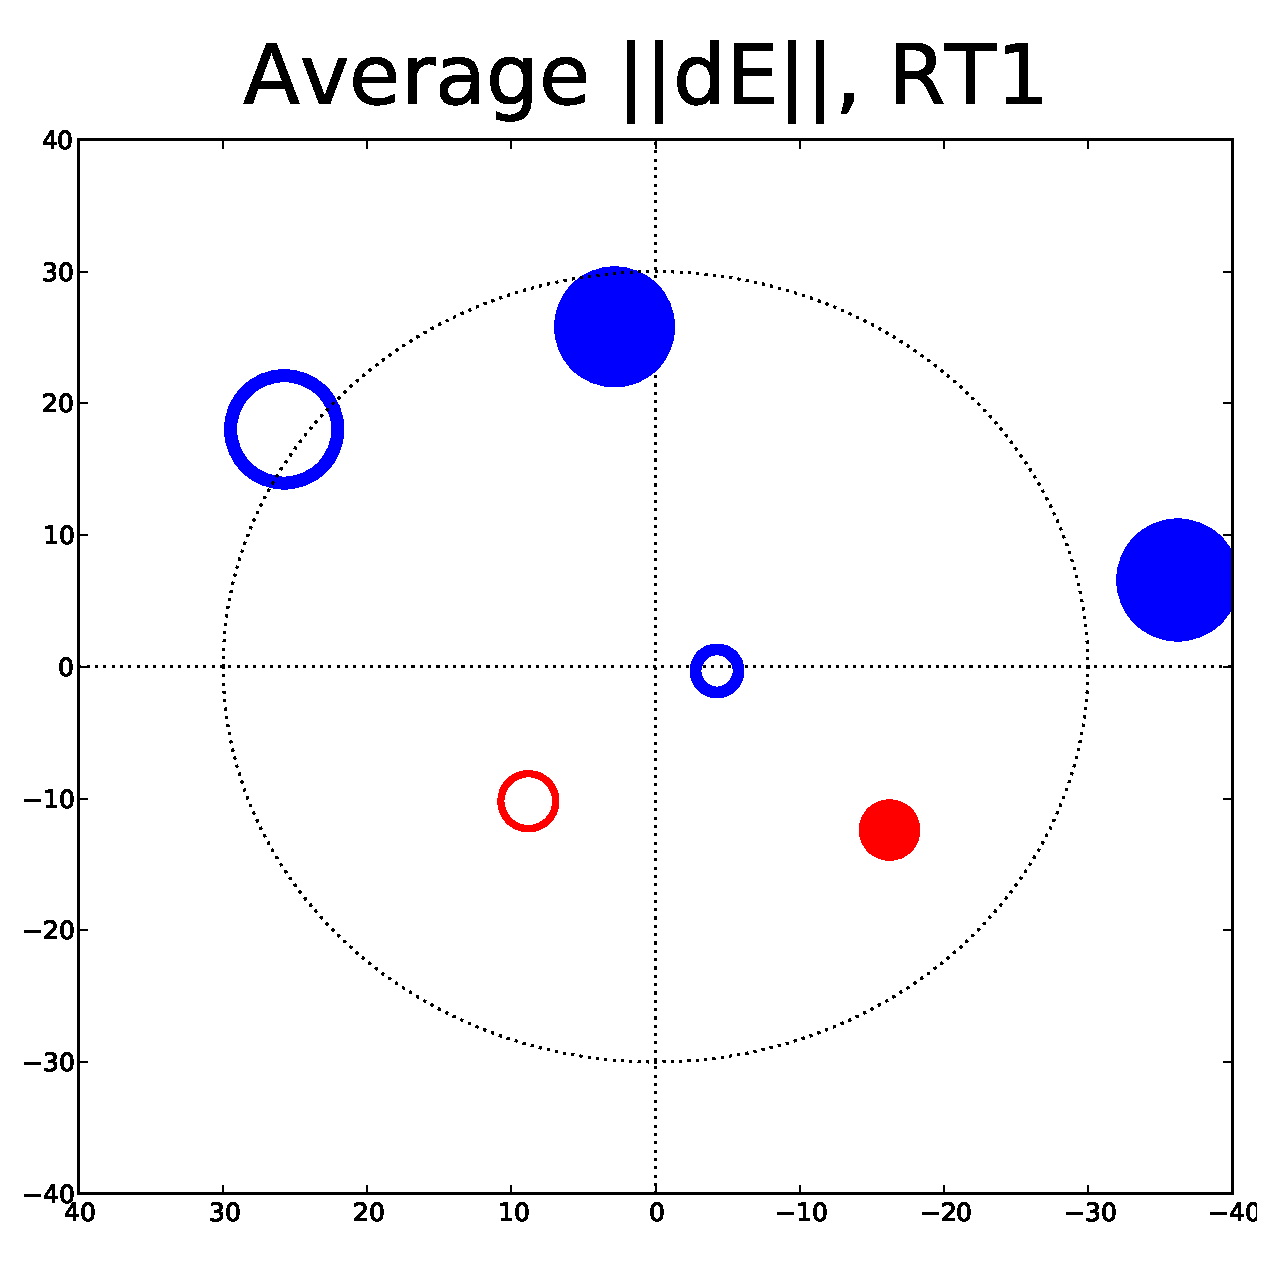
\includegraphics[width=\roguewidth]{o2003_dE_ant1} &
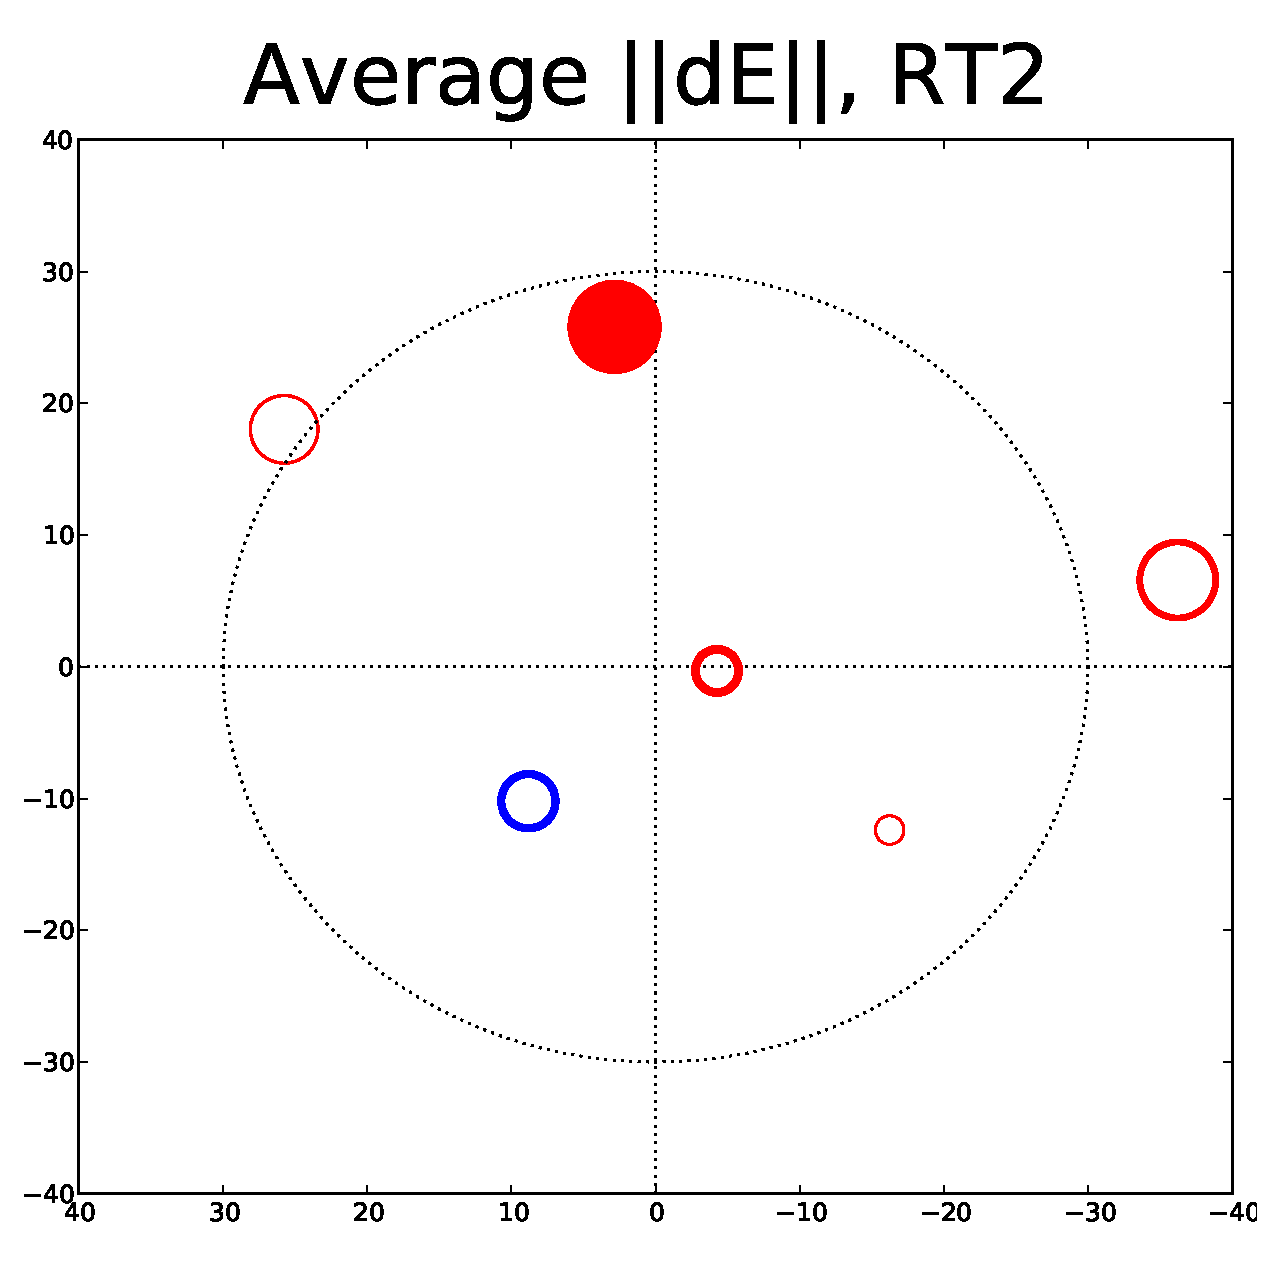
\includegraphics[width=\roguewidth]{o2003_dE_ant2} &
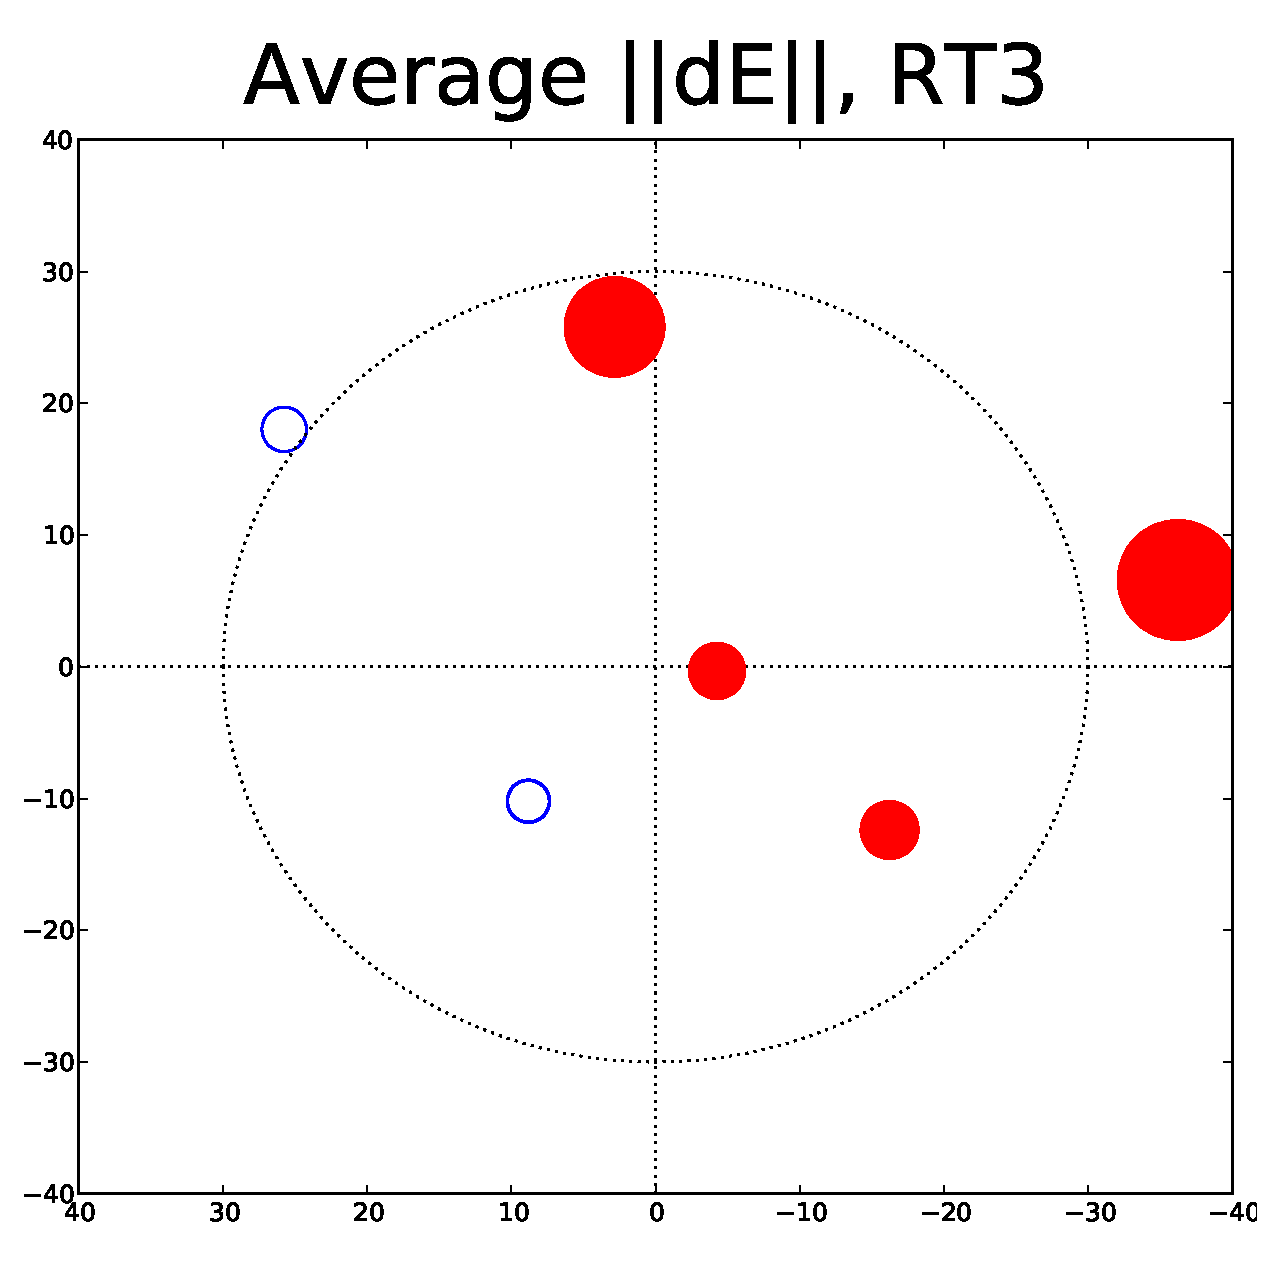
\includegraphics[width=\roguewidth]{o2003_dE_ant3} &
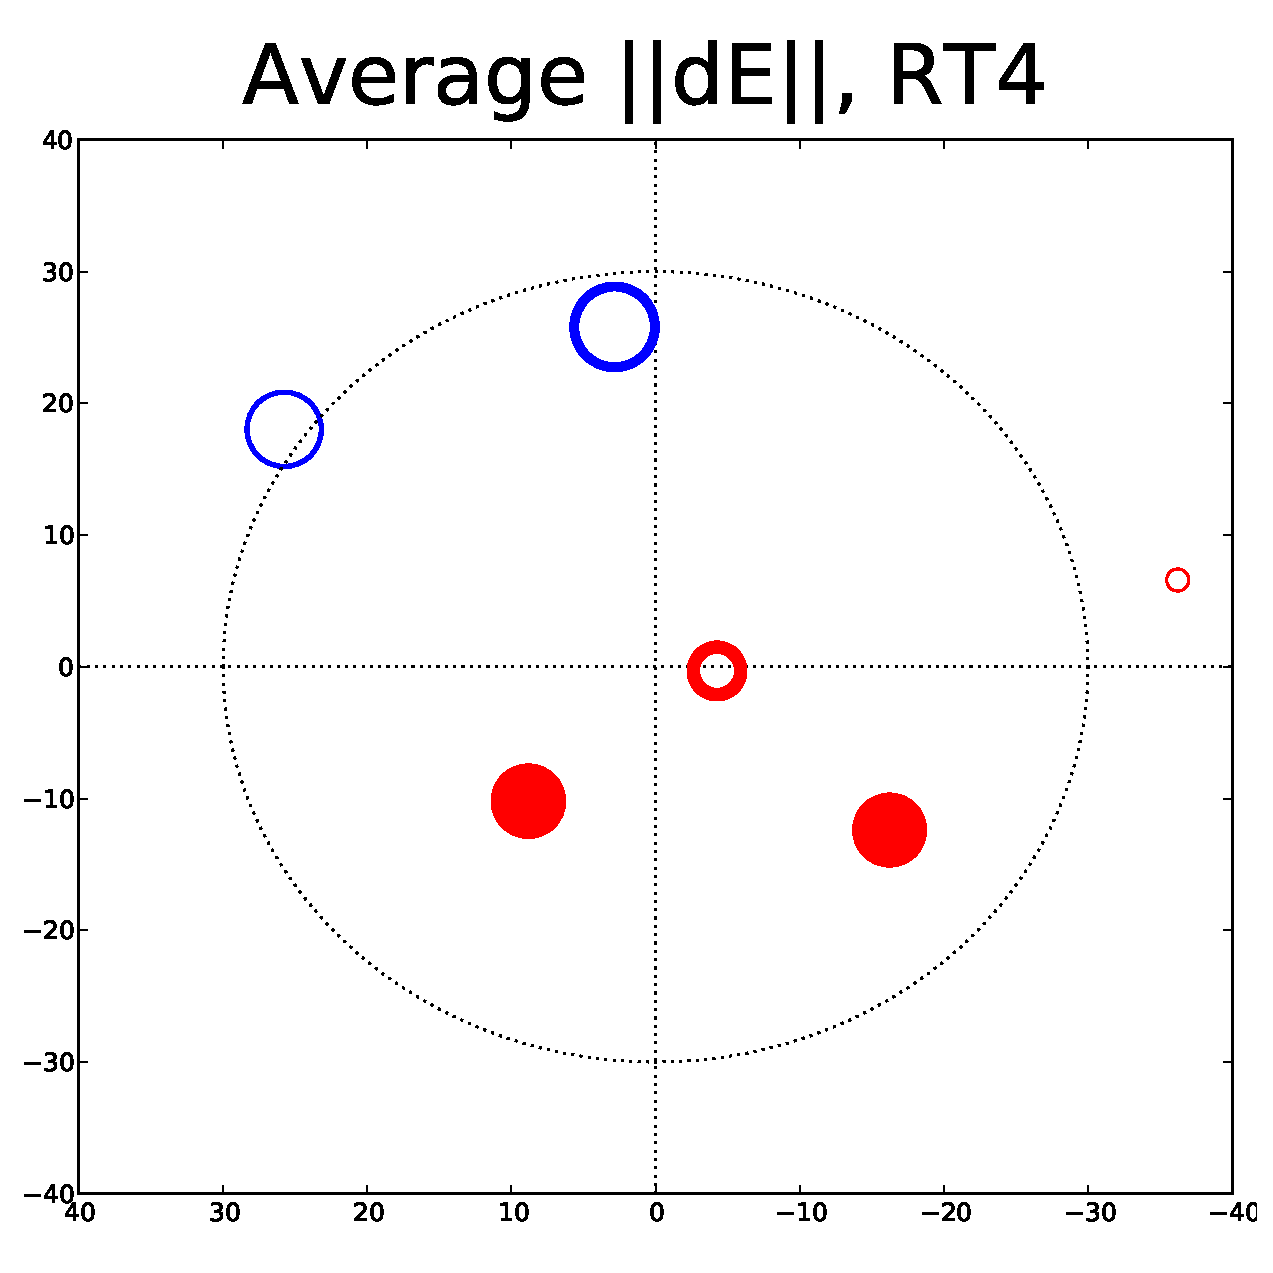
\includegraphics[width=\roguewidth]{o2003_dE_ant4} \\
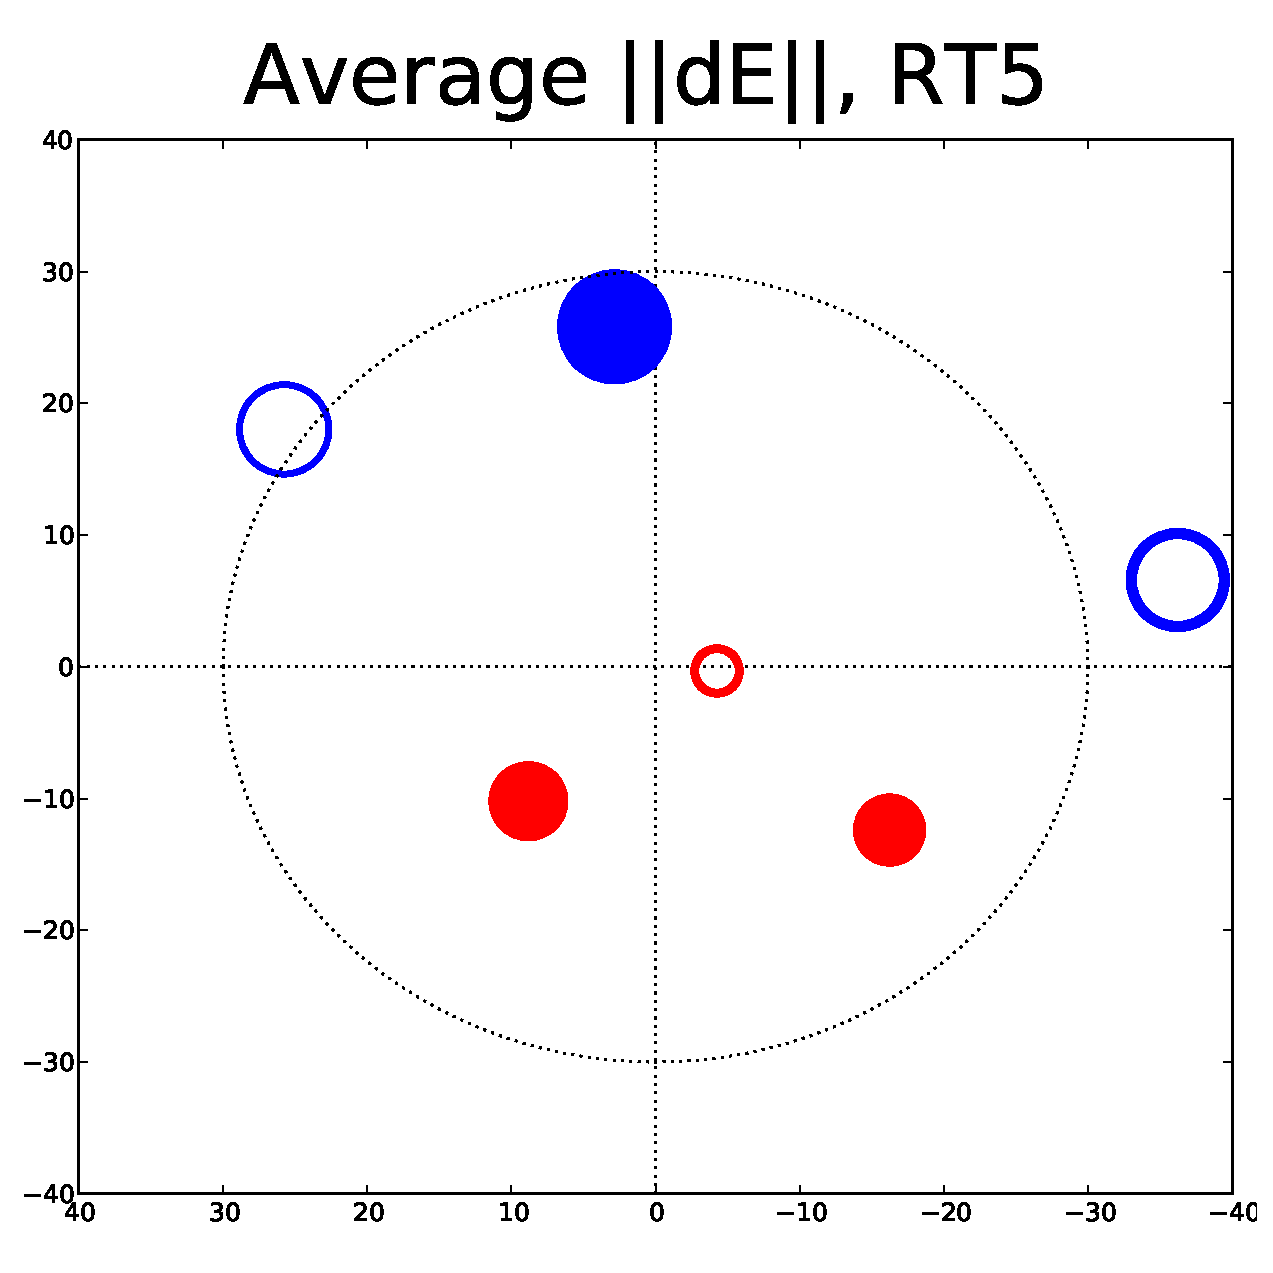
\includegraphics[width=\roguewidth]{o2003_dE_ant5} &
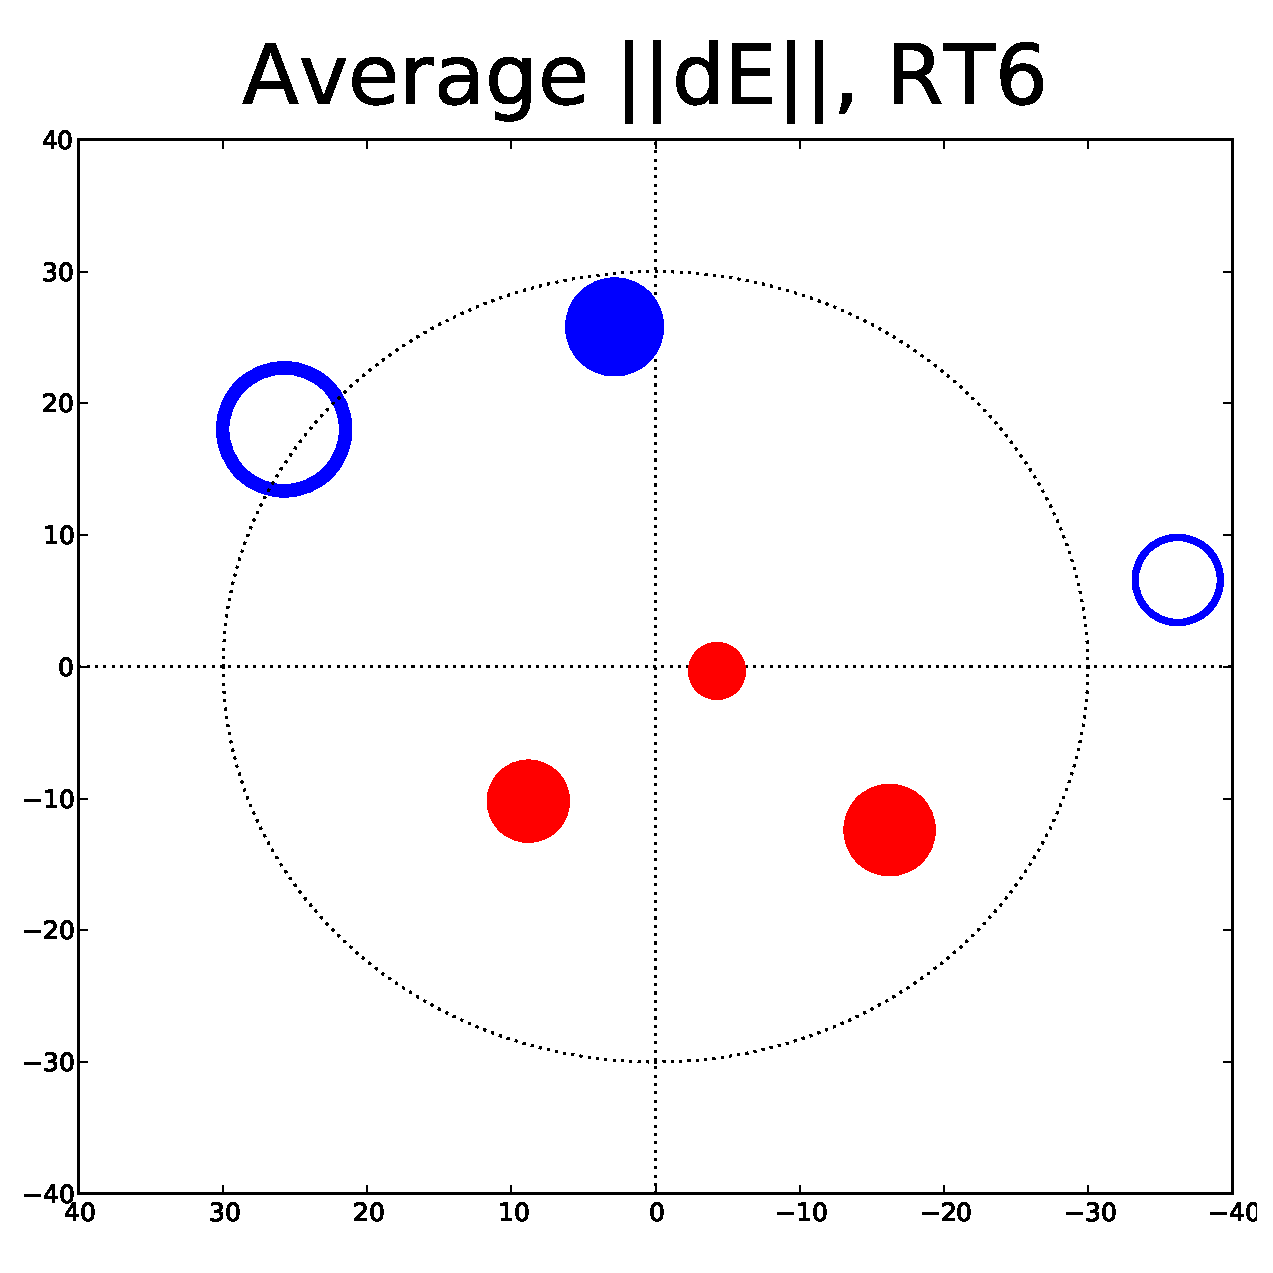
\includegraphics[width=\roguewidth]{o2003_dE_ant6} &
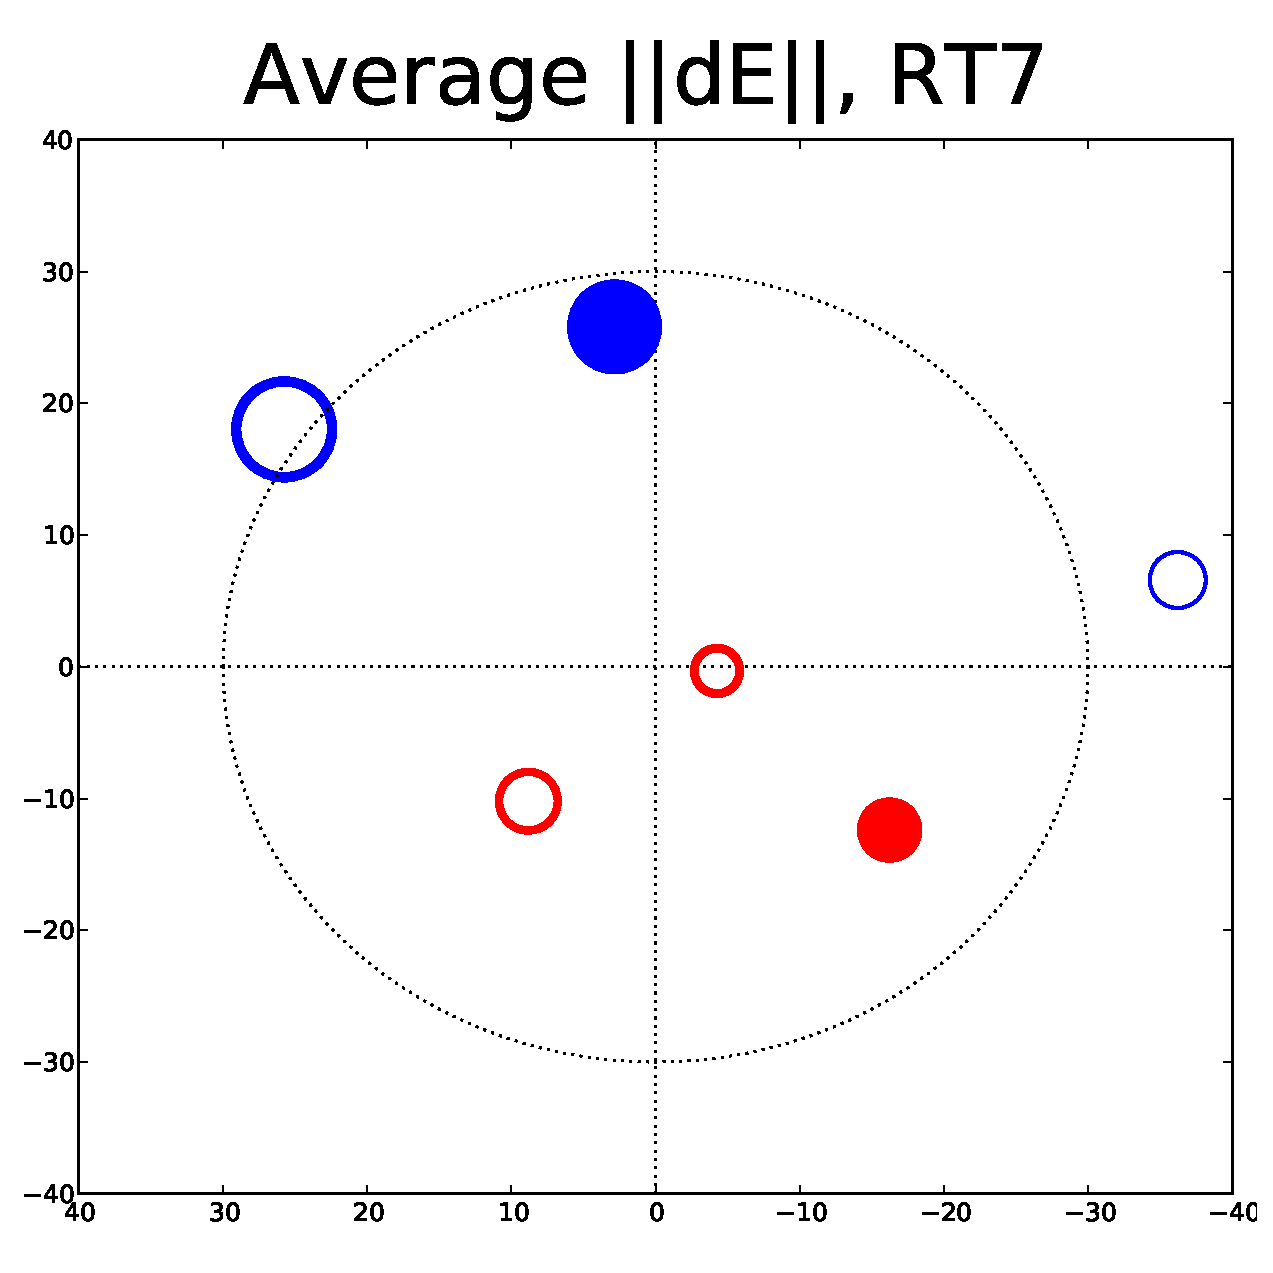
\includegraphics[width=\roguewidth]{o2003_dE_ant7} &
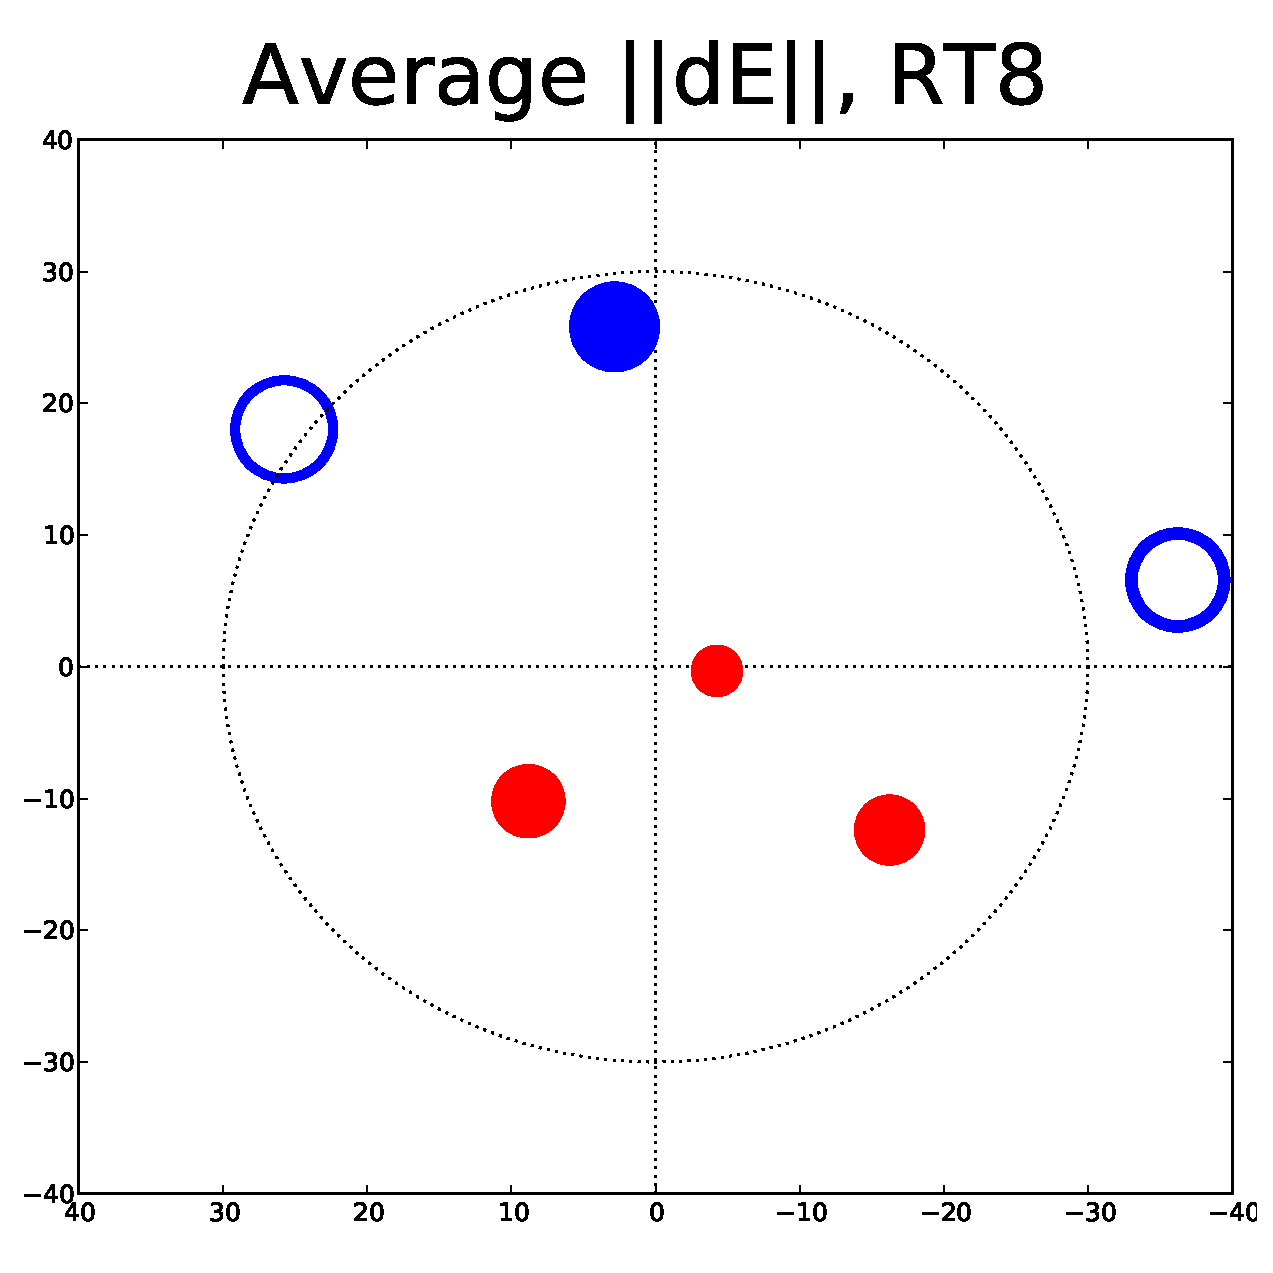
\includegraphics[width=\roguewidth]{o2003_dE_ant8} &
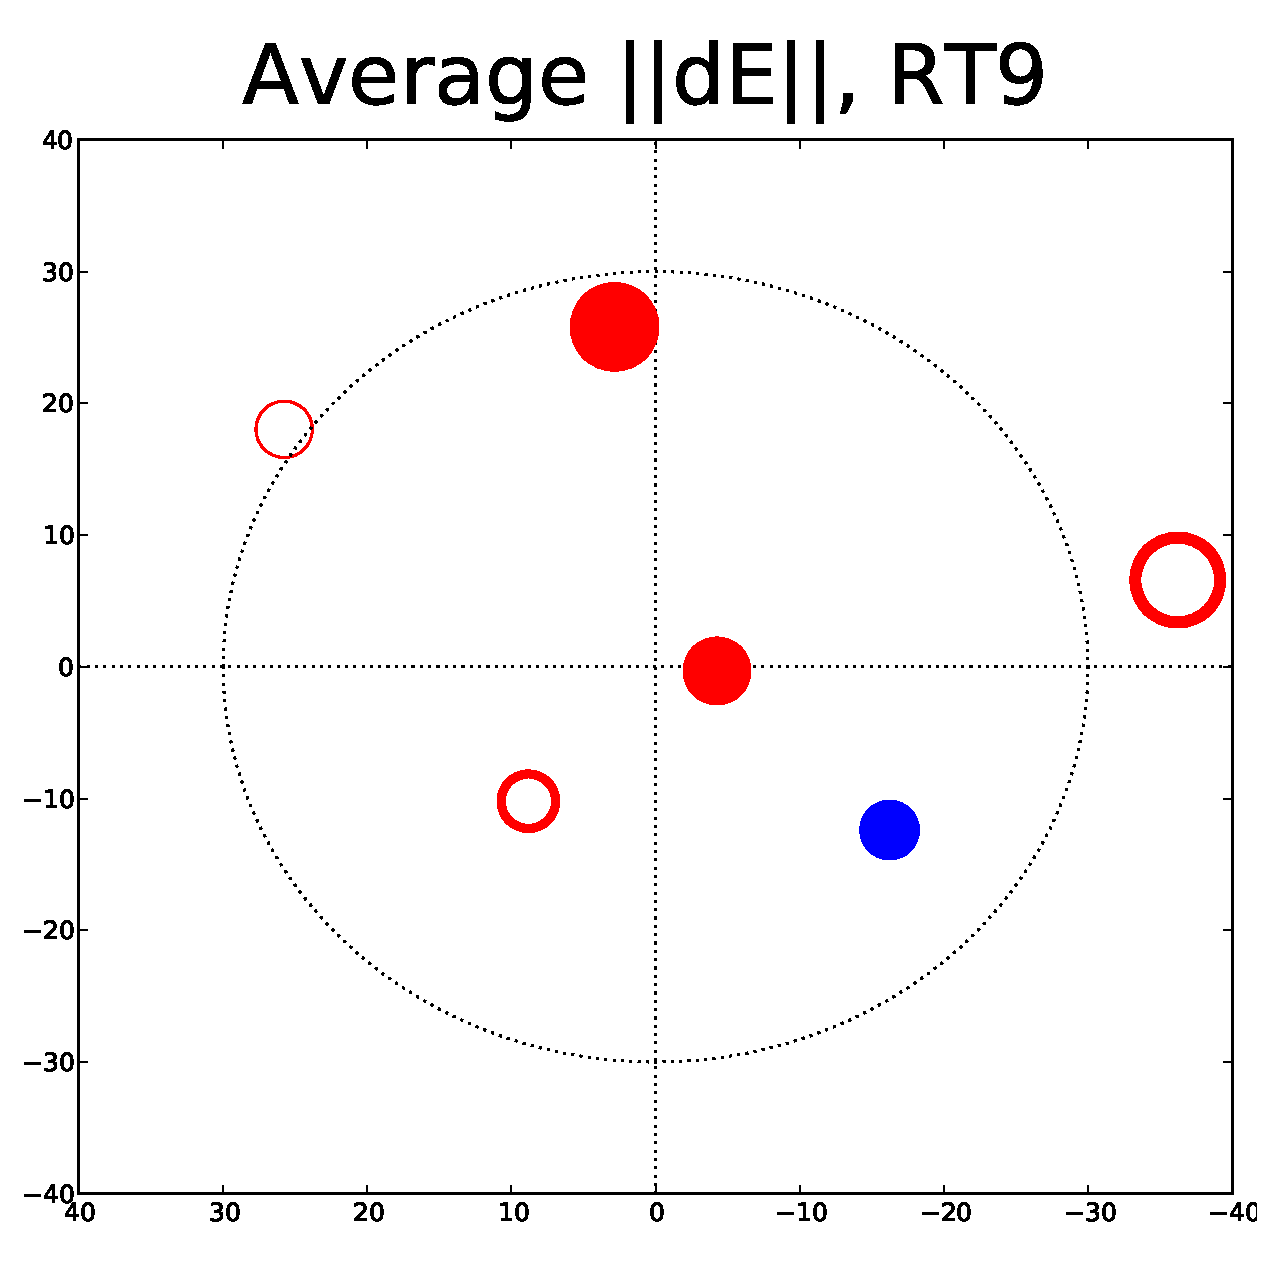
\includegraphics[width=\roguewidth]{o2003_dE_ant9} \\
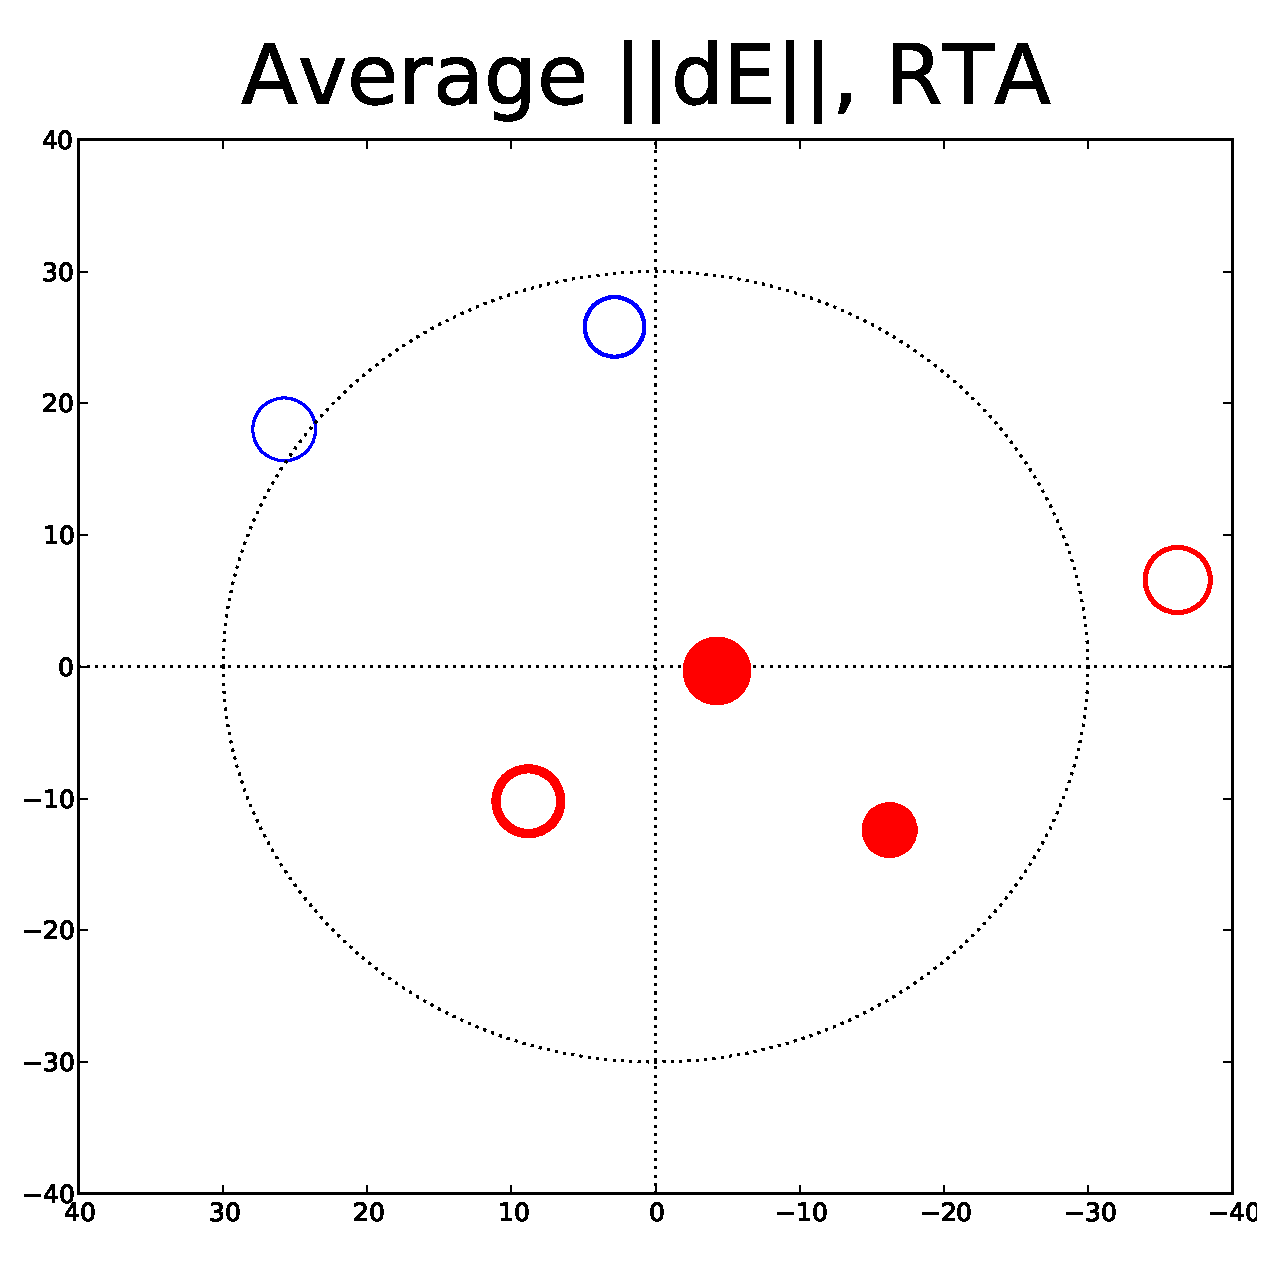
\includegraphics[width=\roguewidth]{o2003_dE_antA} &
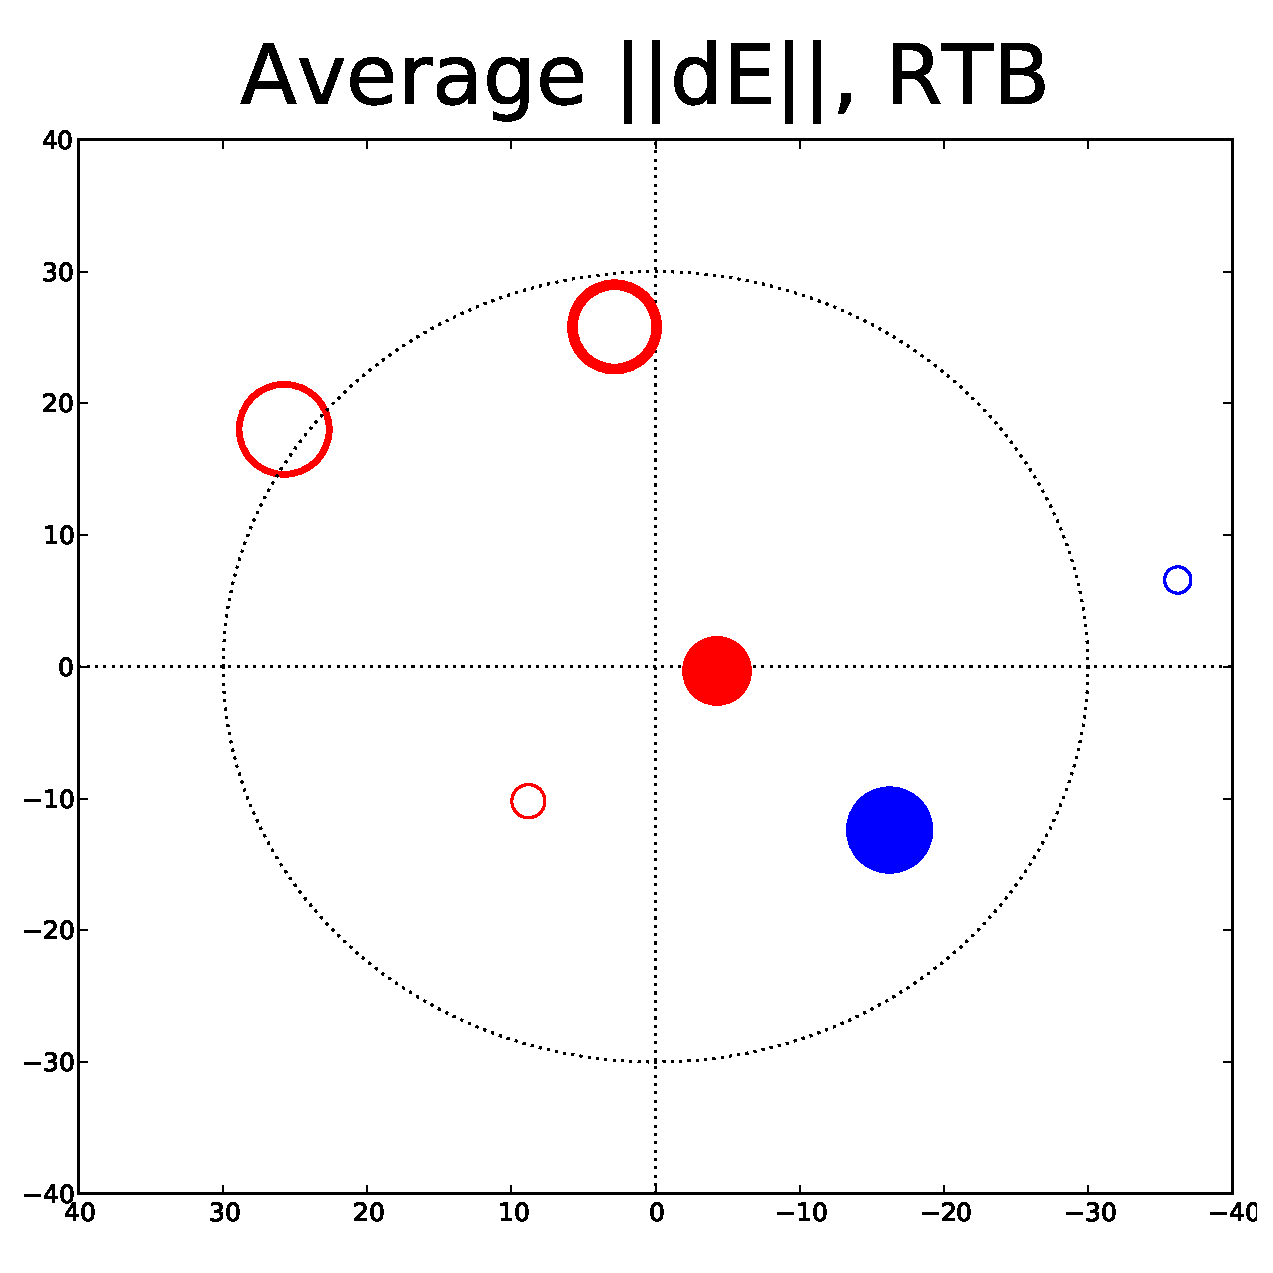
\includegraphics[width=\roguewidth]{o2003_dE_antB} &
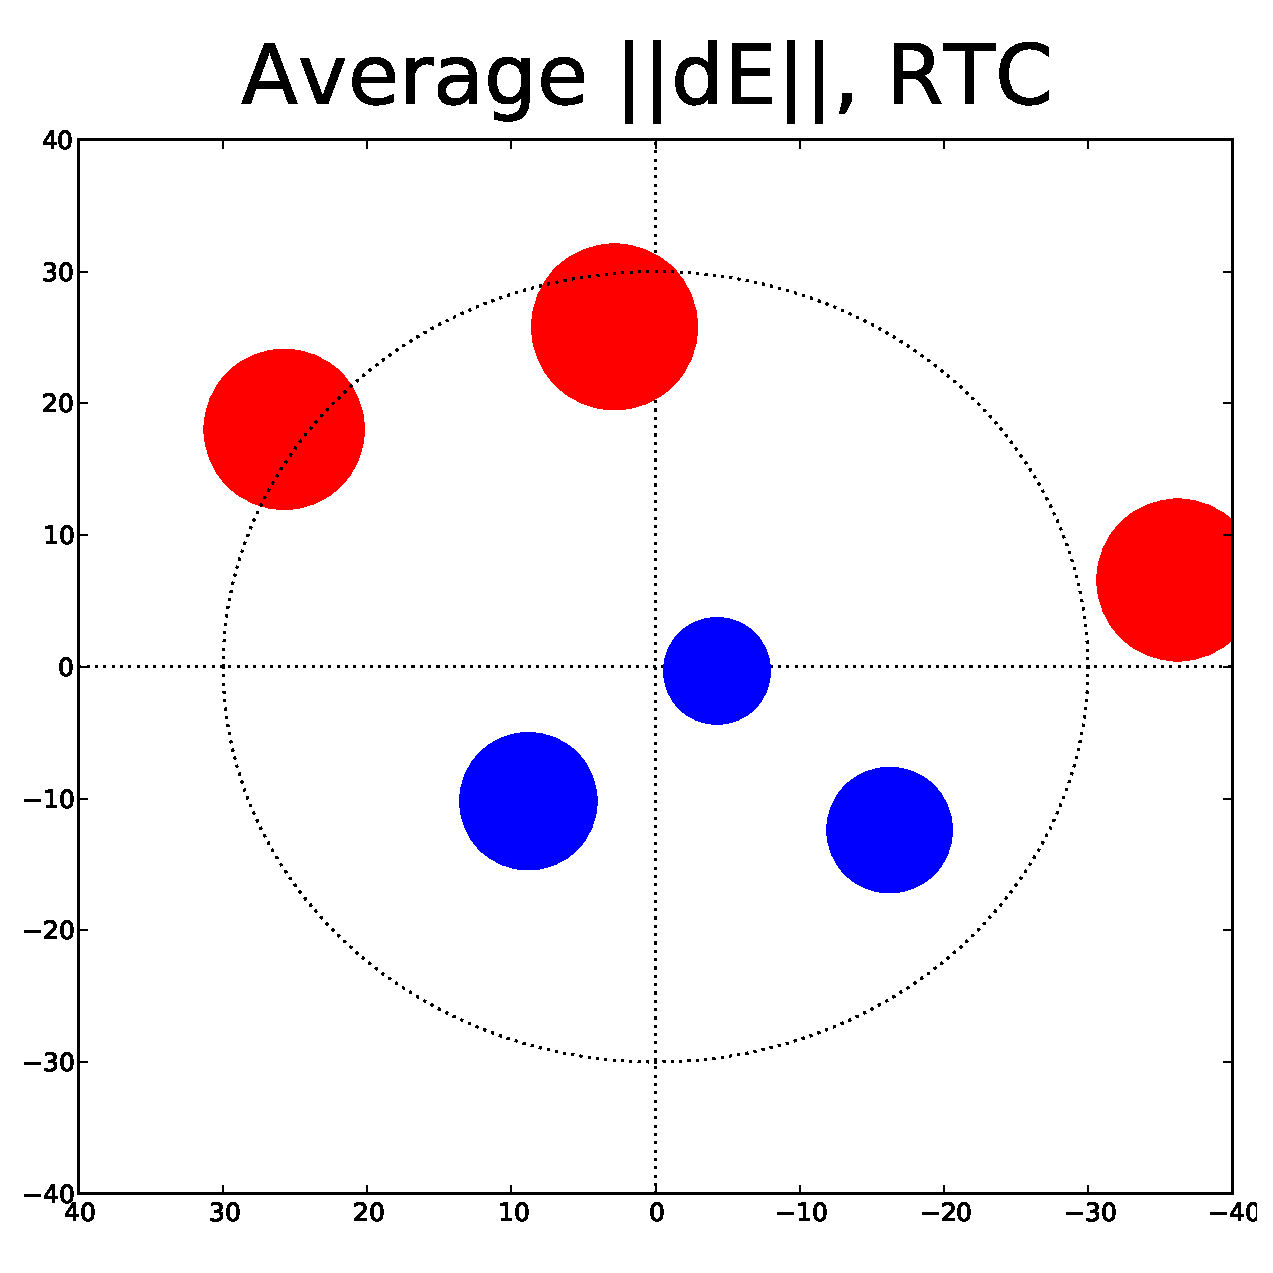
\includegraphics[width=\roguewidth]{o2003_dE_antC} &
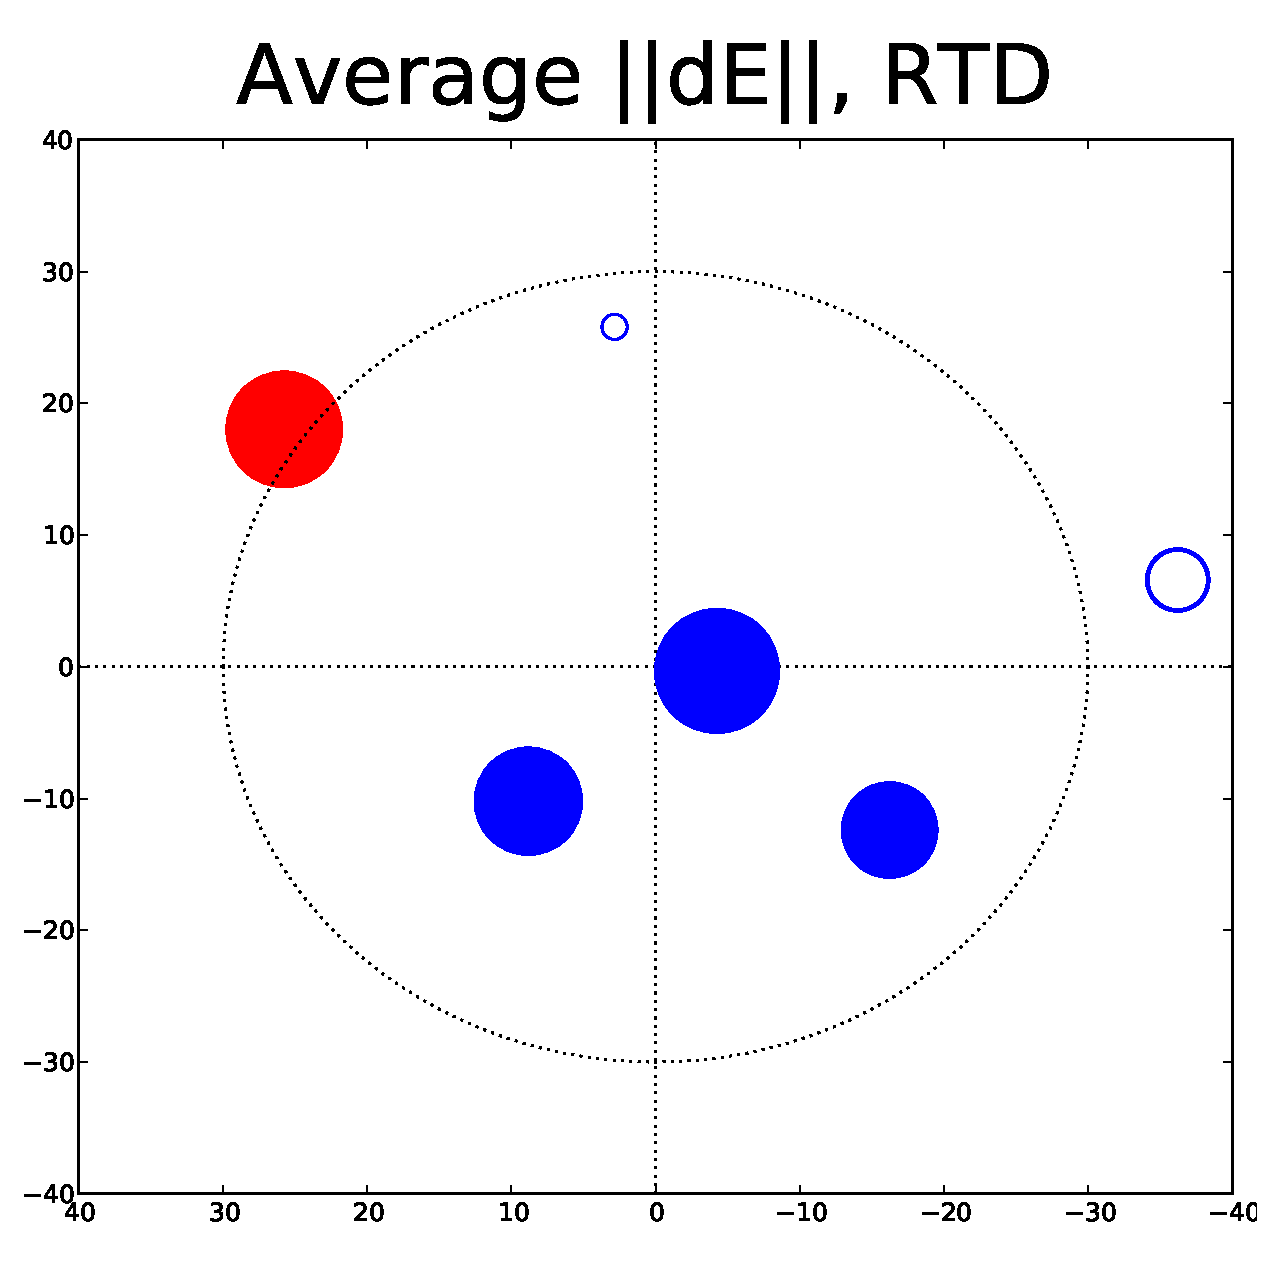
\includegraphics[width=\roguewidth]{o2003_dE_antD} 
\end{tabular}
\caption{\label{fig:rogues-2003}``Rogues gallery'' plot for the 2003 observation. This shows the 12-hour average $||\Delta\jones{E}{}||$ per source, as seen by each antenna. Blue circles correspond to values of $||\Delta\jones{E}{}||>1$, red circles to values of $||\Delta\jones{E}{}||<1$, and areas are proportional to $|\,||\Delta\jones{E}{}||-1\,|$. Line thickness indicates the statistical significance of $|\,||\Delta\jones{E}{}||-1\,|$; filled circles are for detections of over $3\sigma$. The large grid circle is at radius $30\arcmin$.}
\end{figure}

\begin{figure}
\centering
%\sidecaption
\begin{tabular}{@{}c@{}c@{}c@{}c@{}c@{}}
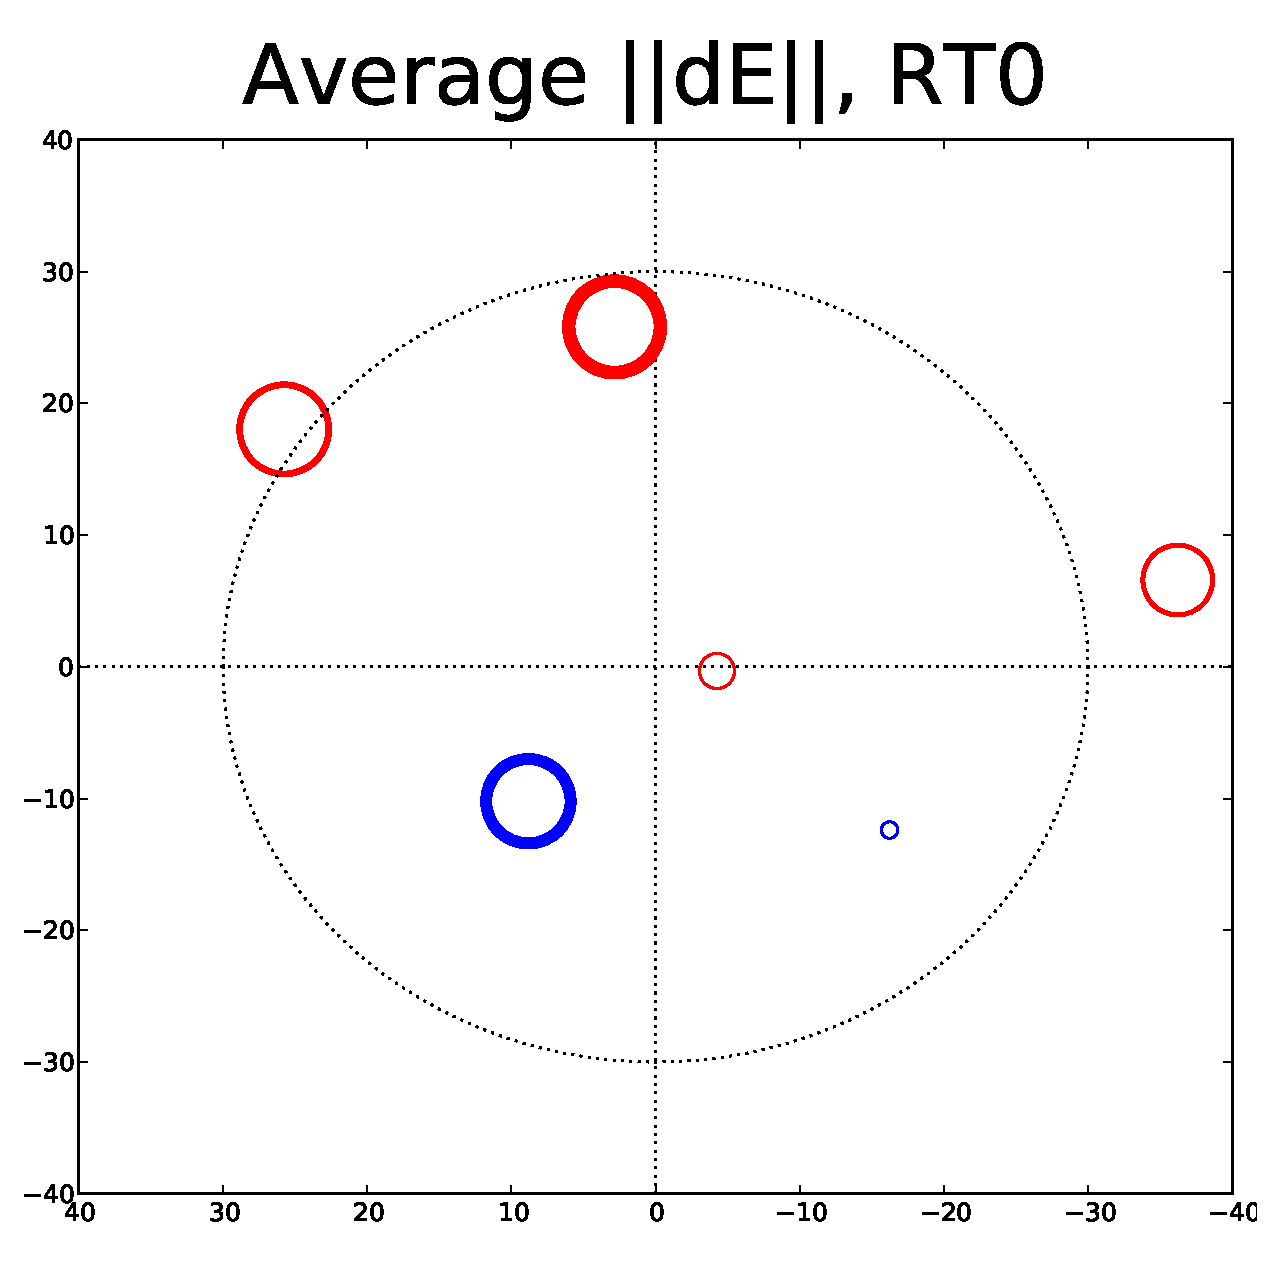
\includegraphics[width=\roguewidth]{o2006_dE_ant0} &
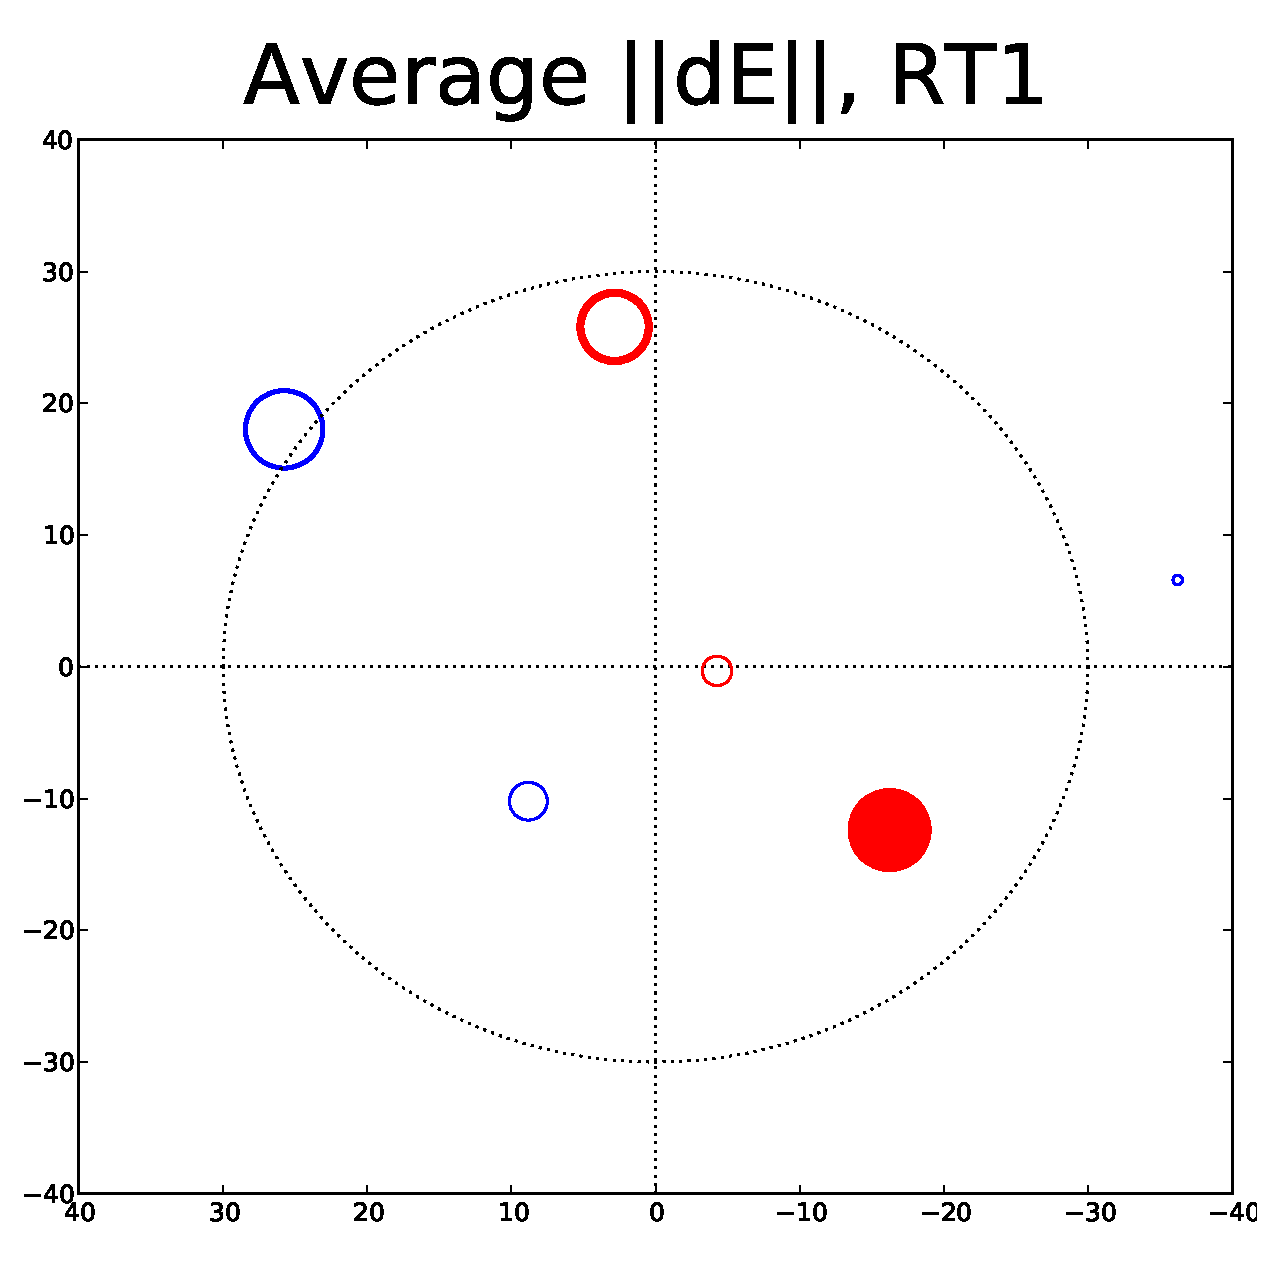
\includegraphics[width=\roguewidth]{o2006_dE_ant1} &
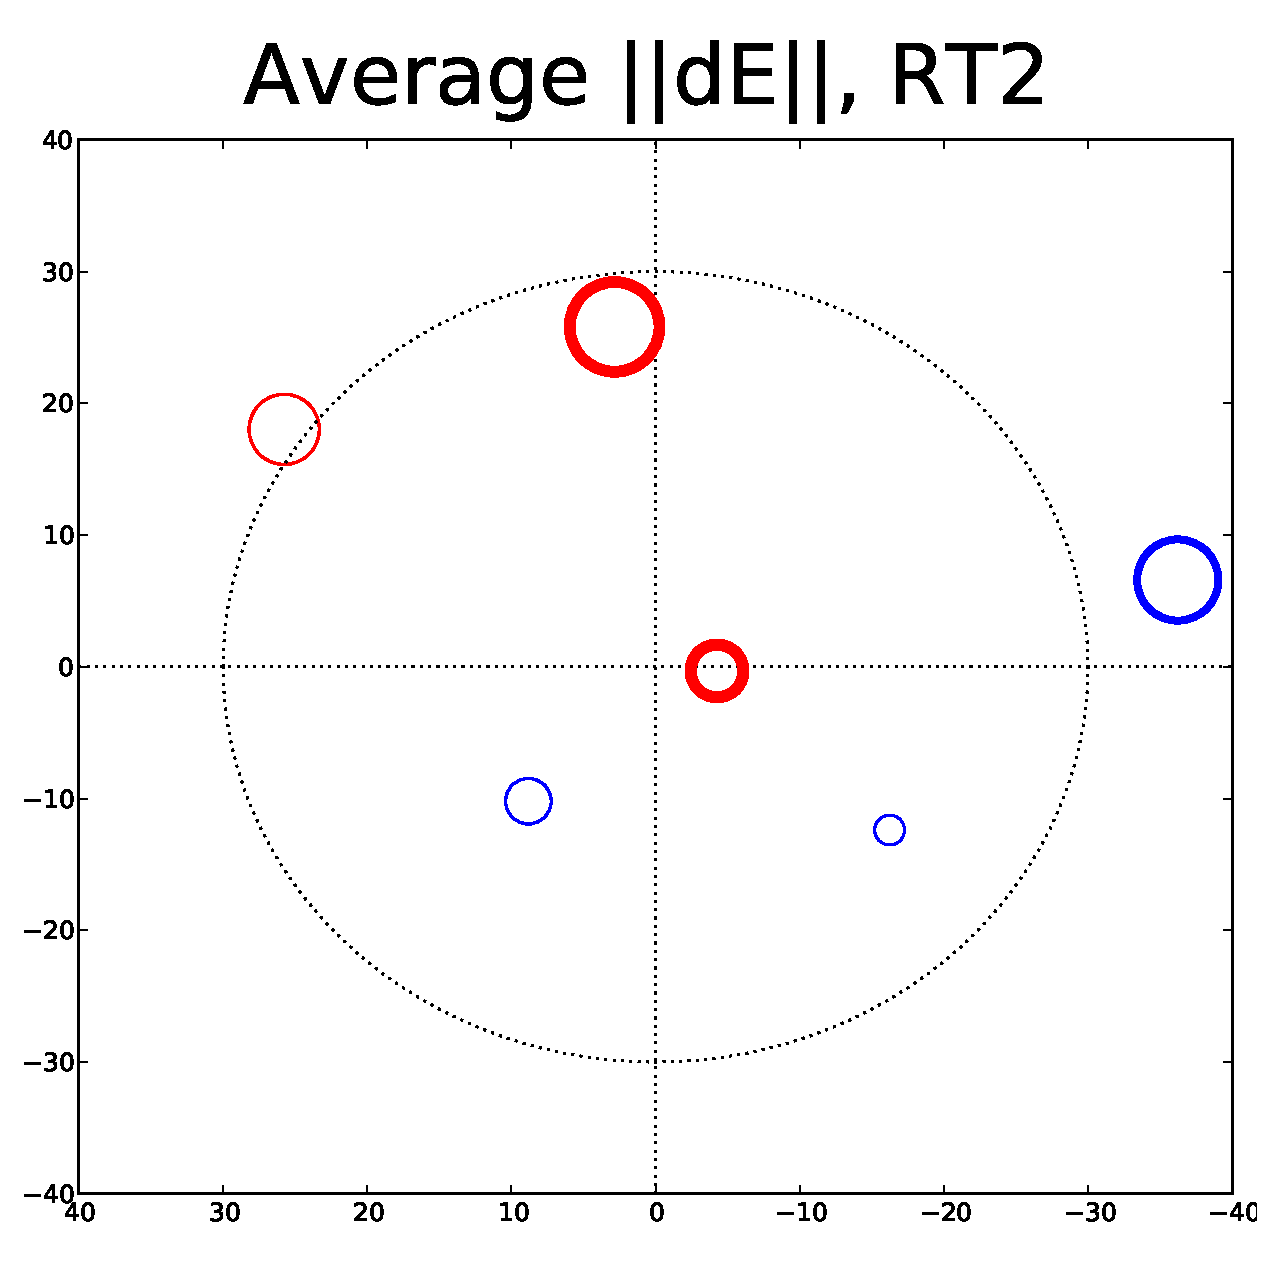
\includegraphics[width=\roguewidth]{o2006_dE_ant2} &
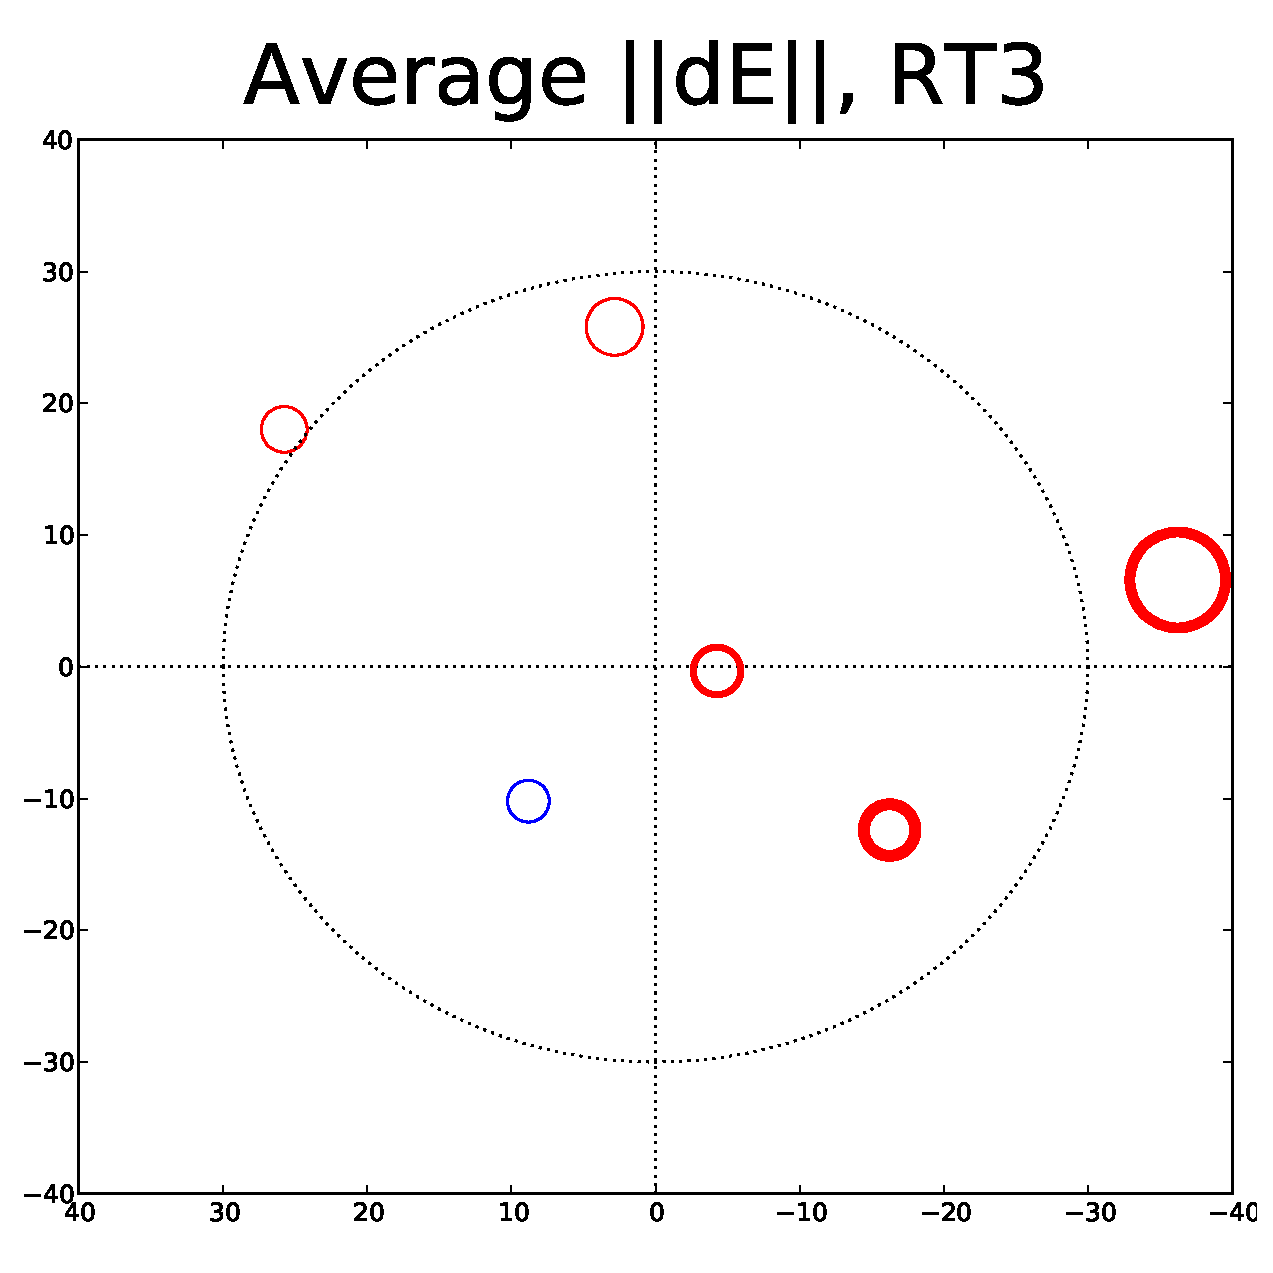
\includegraphics[width=\roguewidth]{o2006_dE_ant3} &
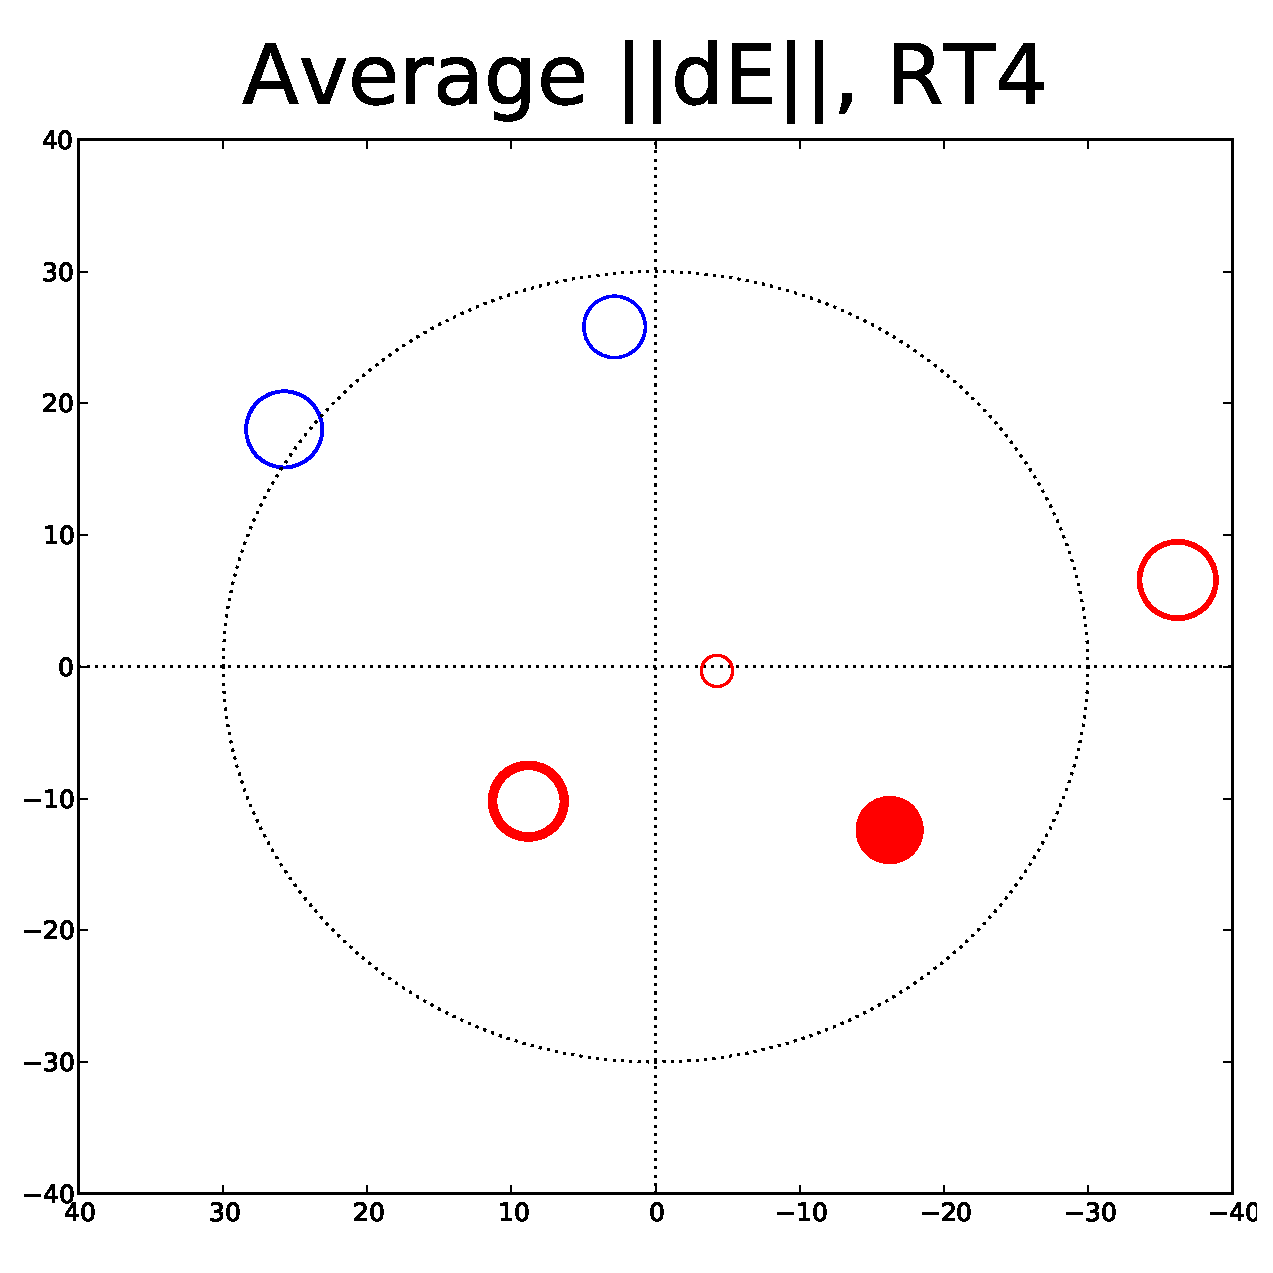
\includegraphics[width=\roguewidth]{o2006_dE_ant4} \\
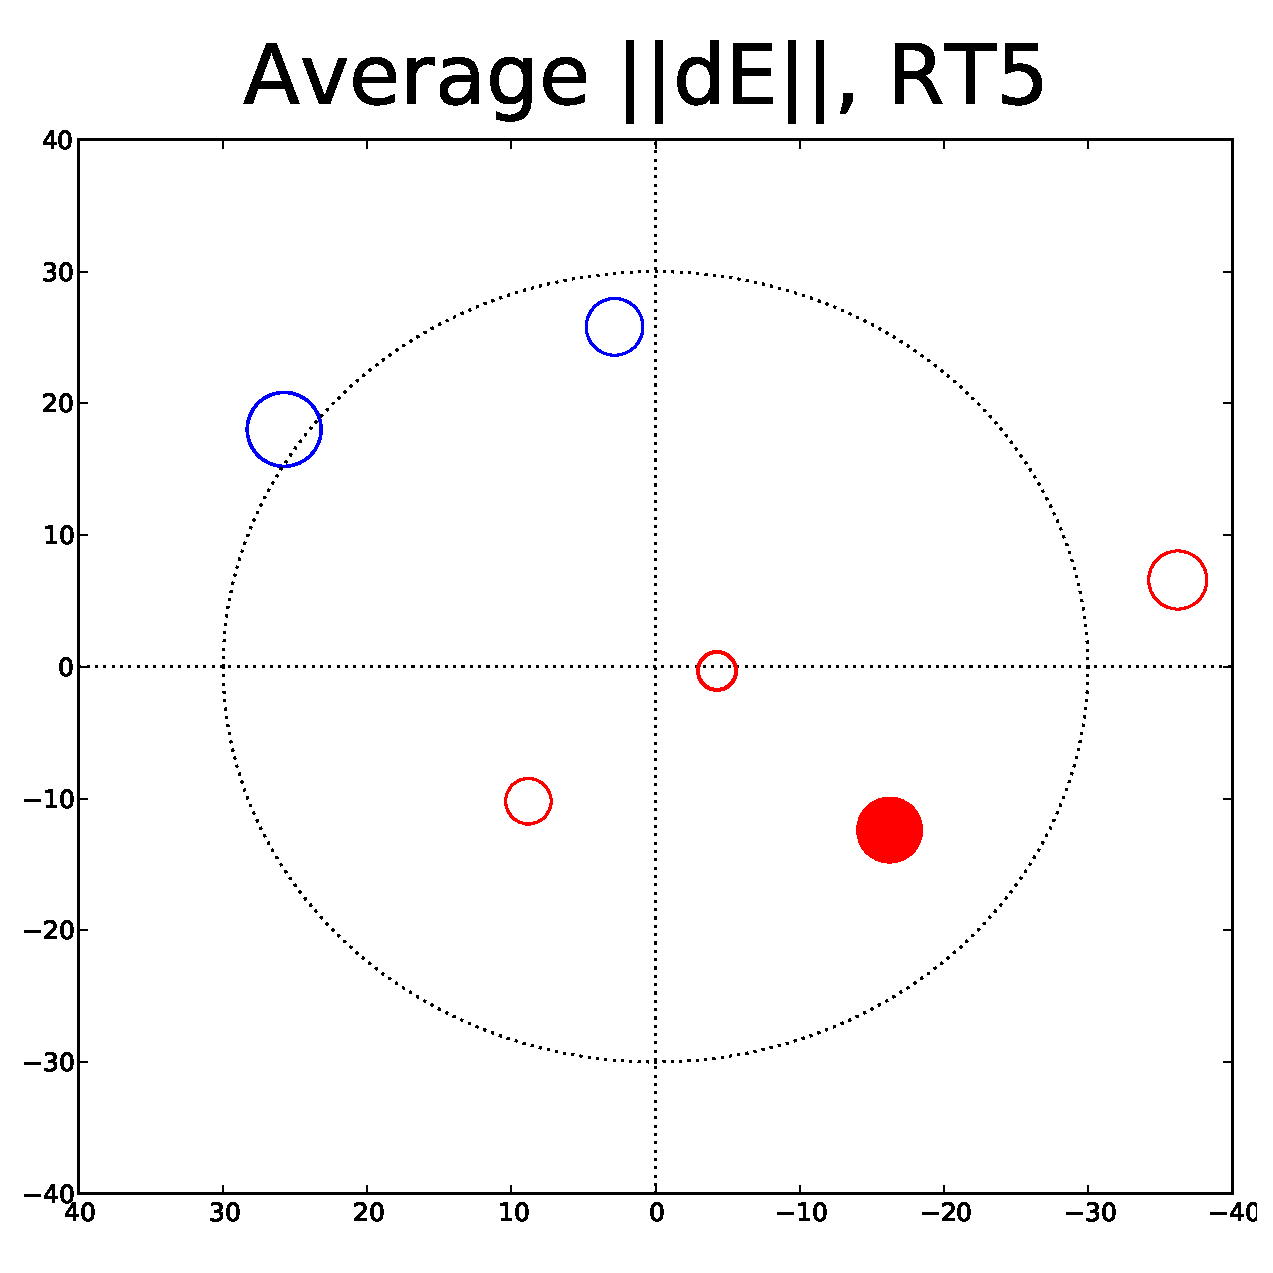
\includegraphics[width=\roguewidth]{o2006_dE_ant5} &
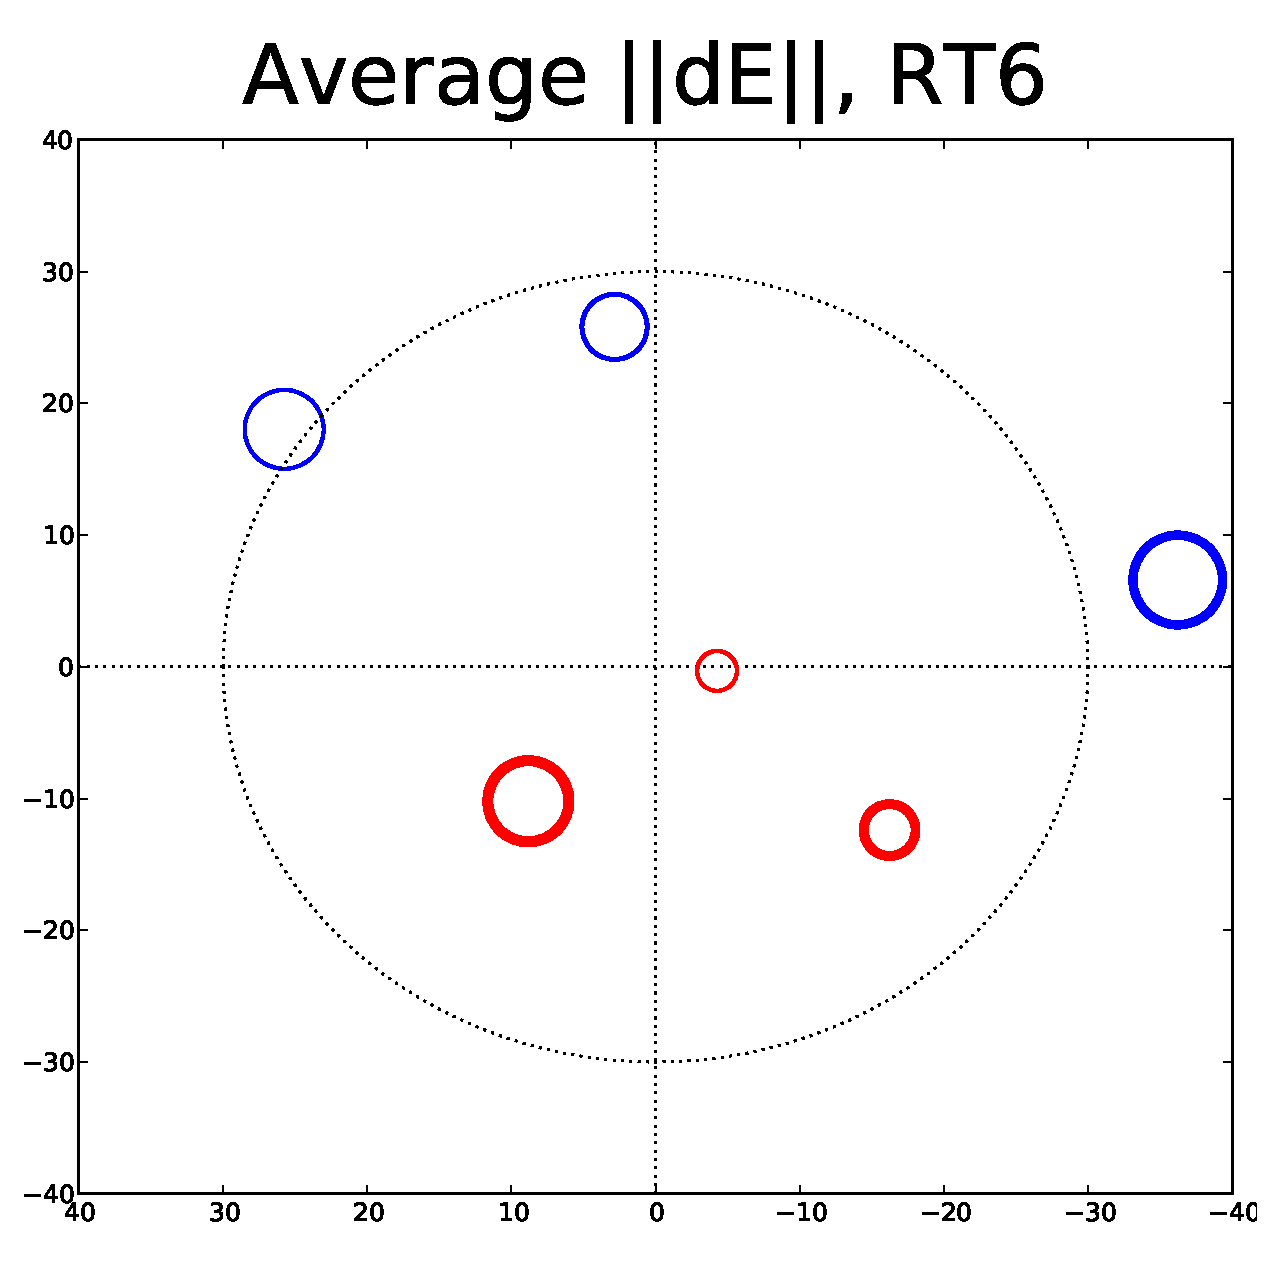
\includegraphics[width=\roguewidth]{o2006_dE_ant6} &
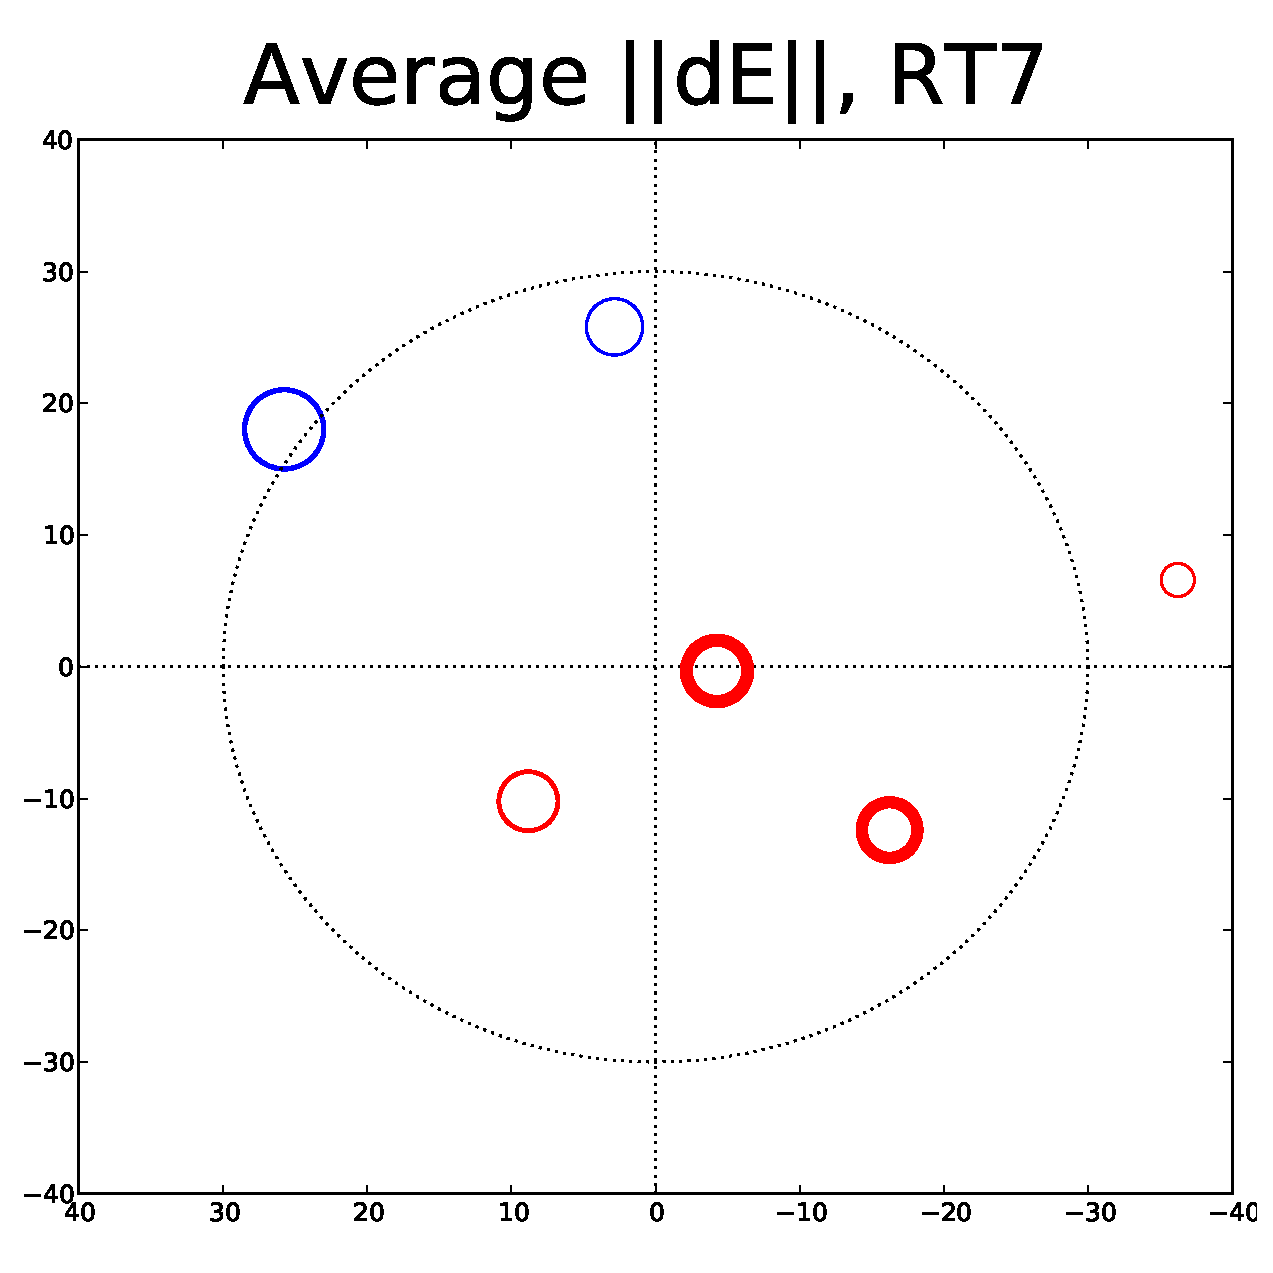
\includegraphics[width=\roguewidth]{o2006_dE_ant7} &
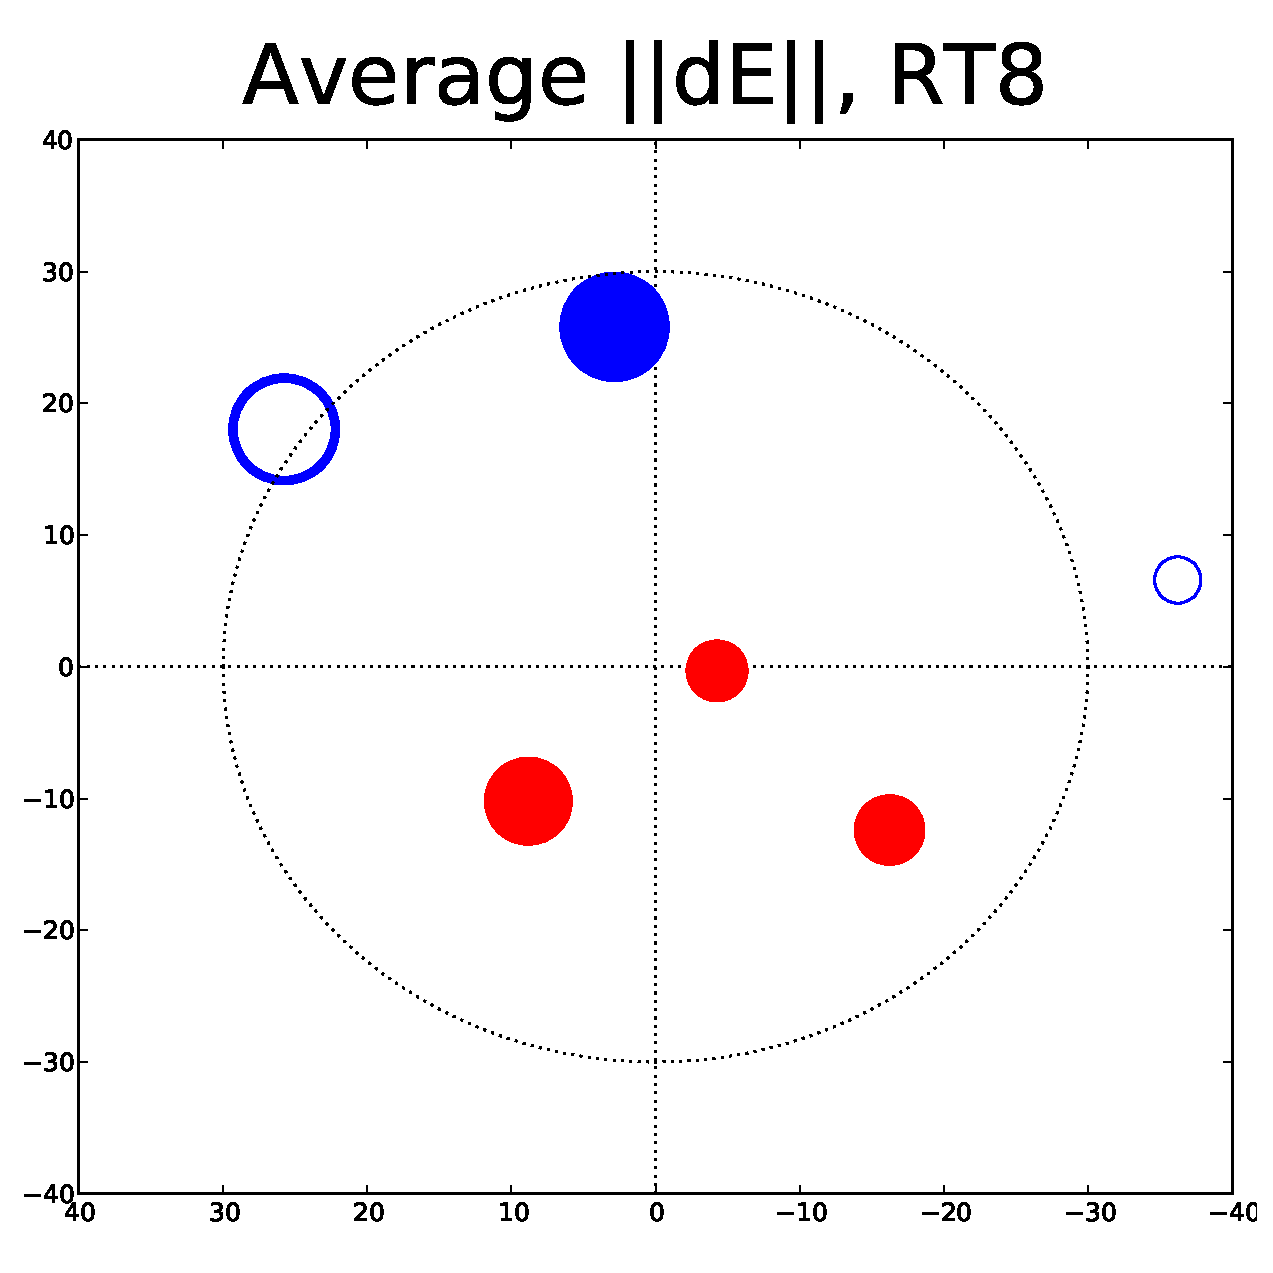
\includegraphics[width=\roguewidth]{o2006_dE_ant8} &
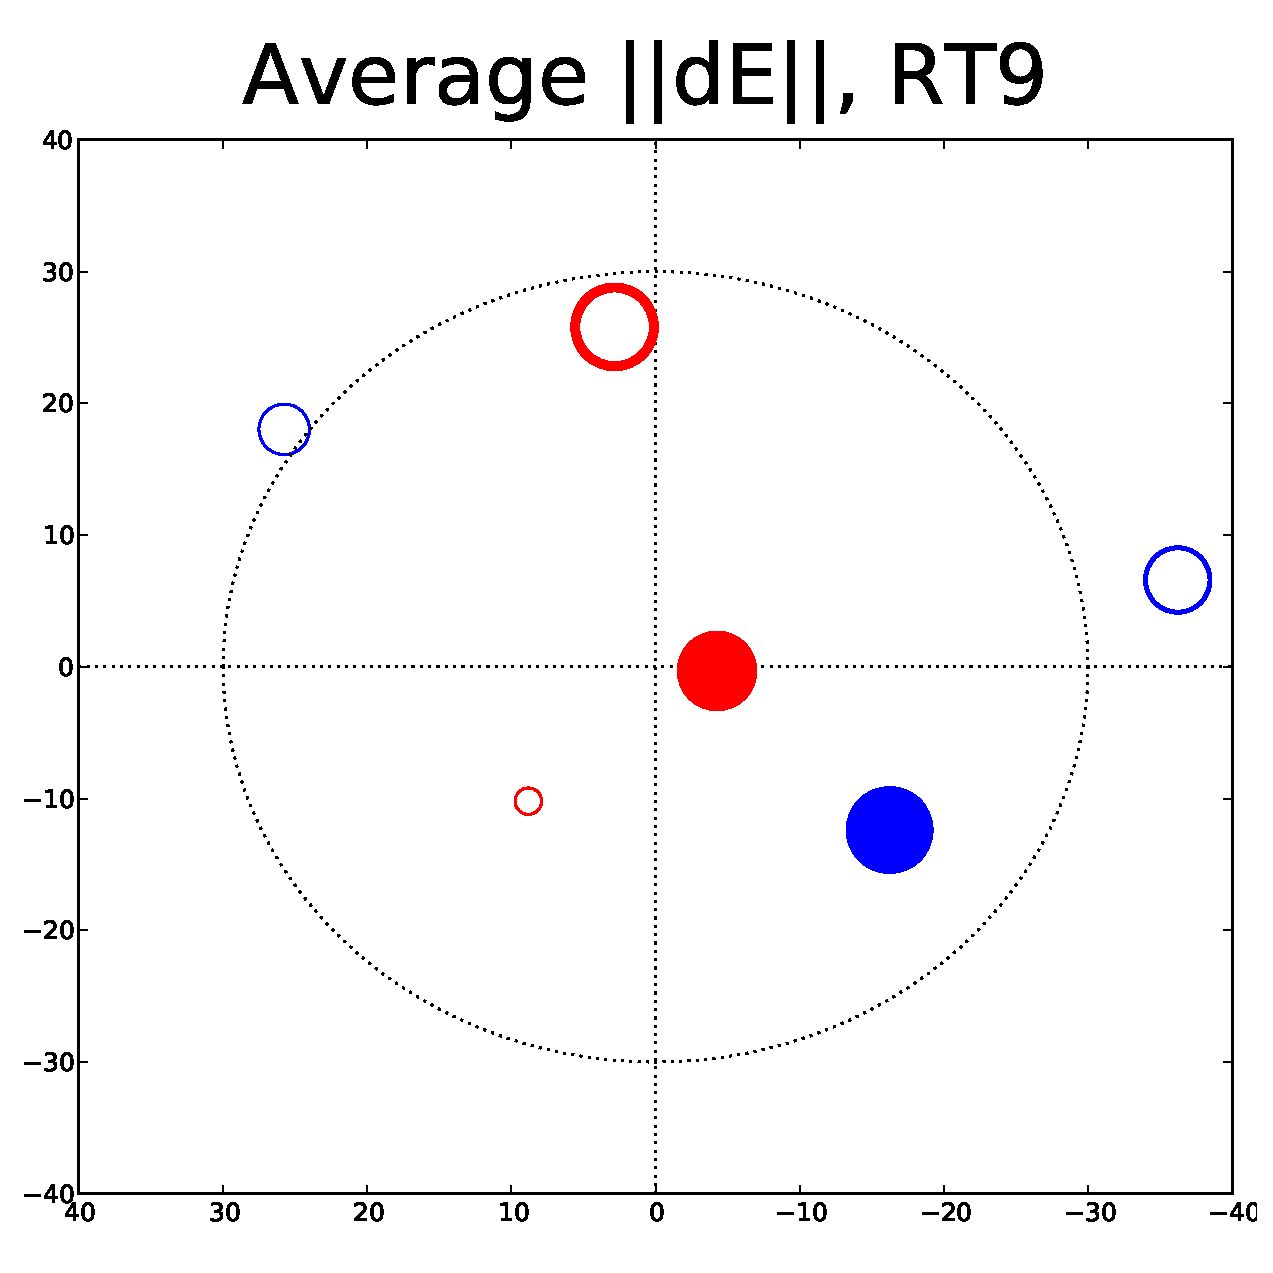
\includegraphics[width=\roguewidth]{o2006_dE_ant9} \\
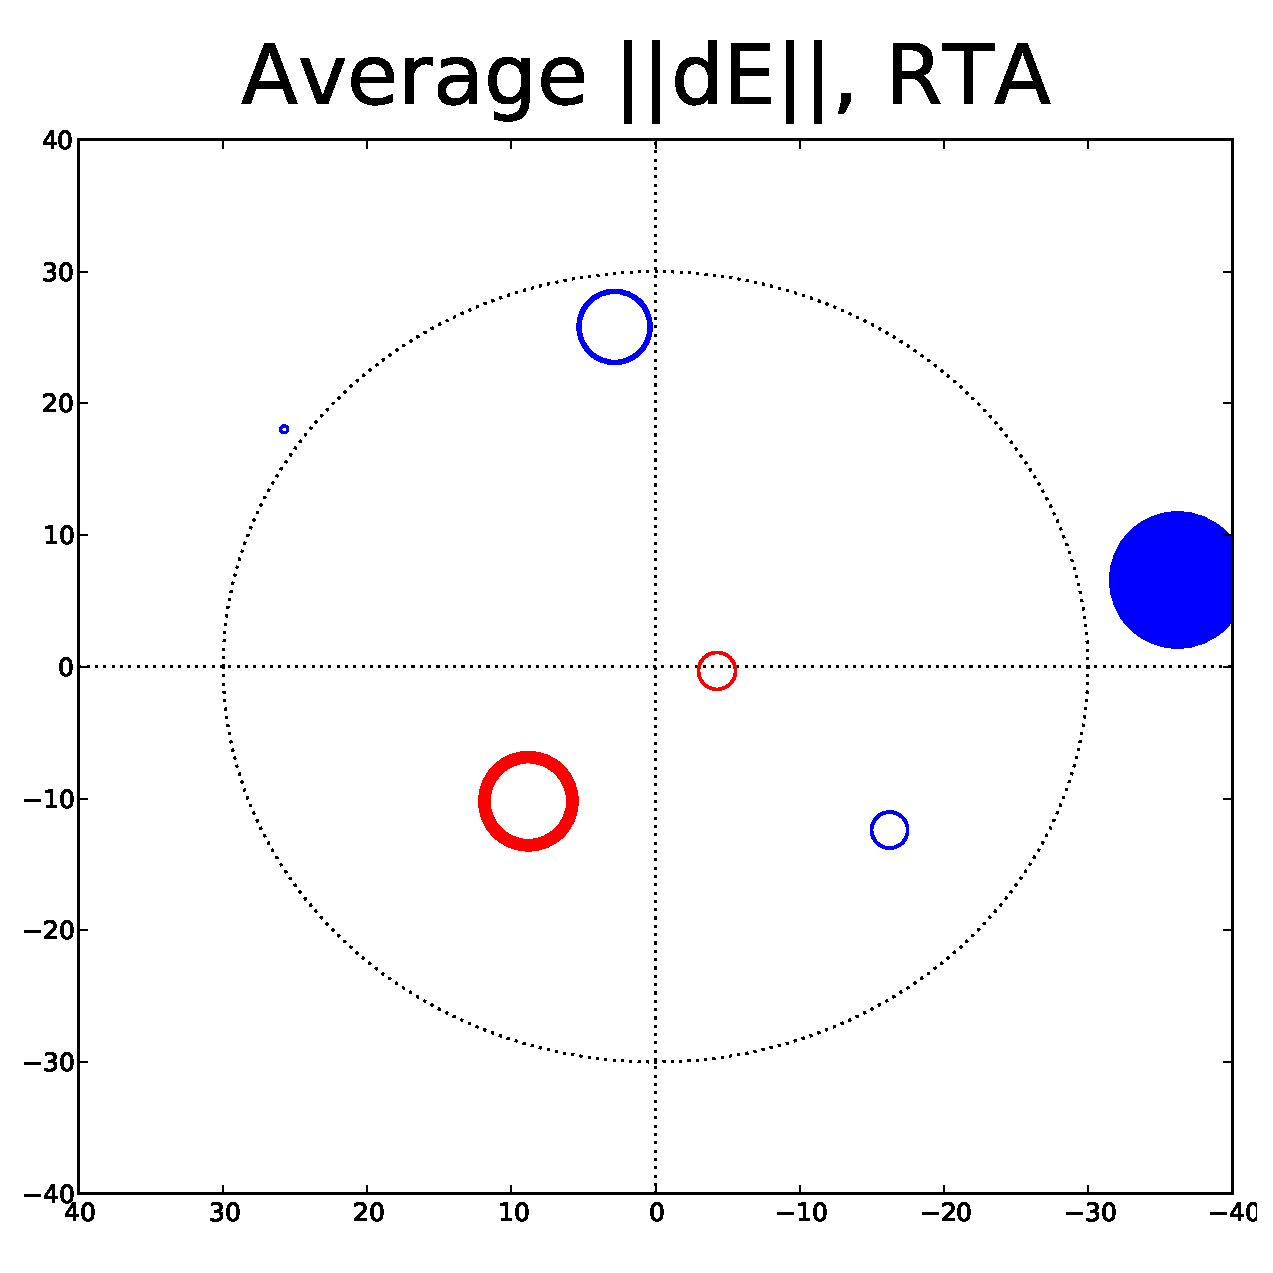
\includegraphics[width=\roguewidth]{o2006_dE_antA} &
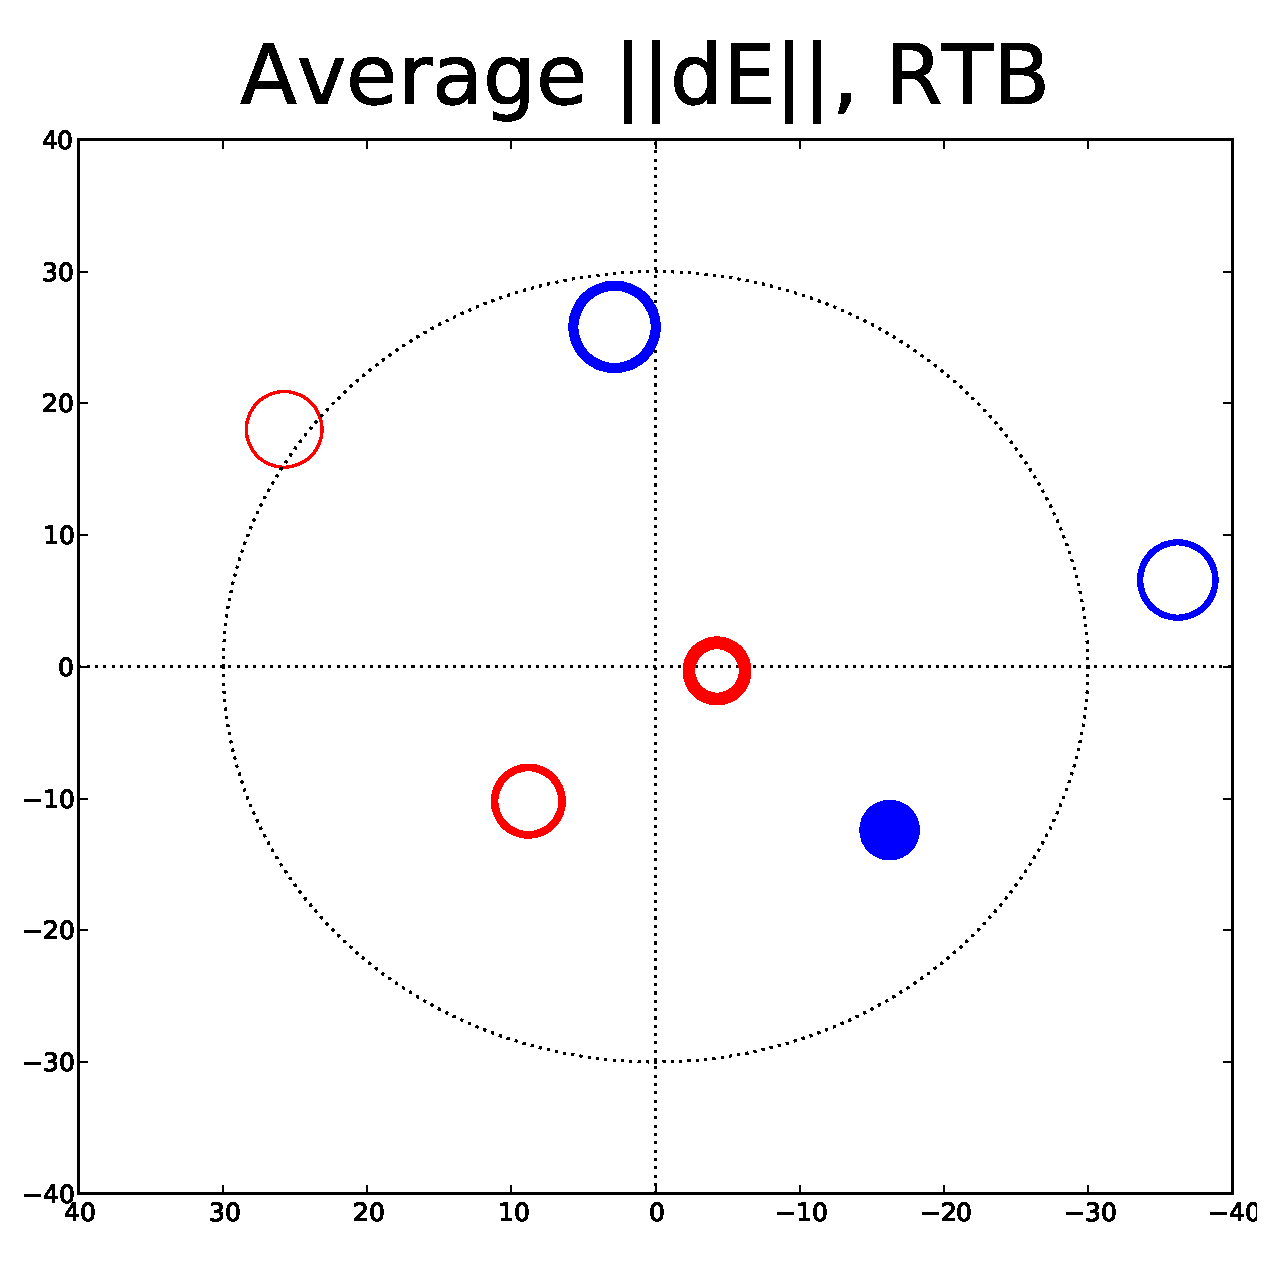
\includegraphics[width=\roguewidth]{o2006_dE_antB} &
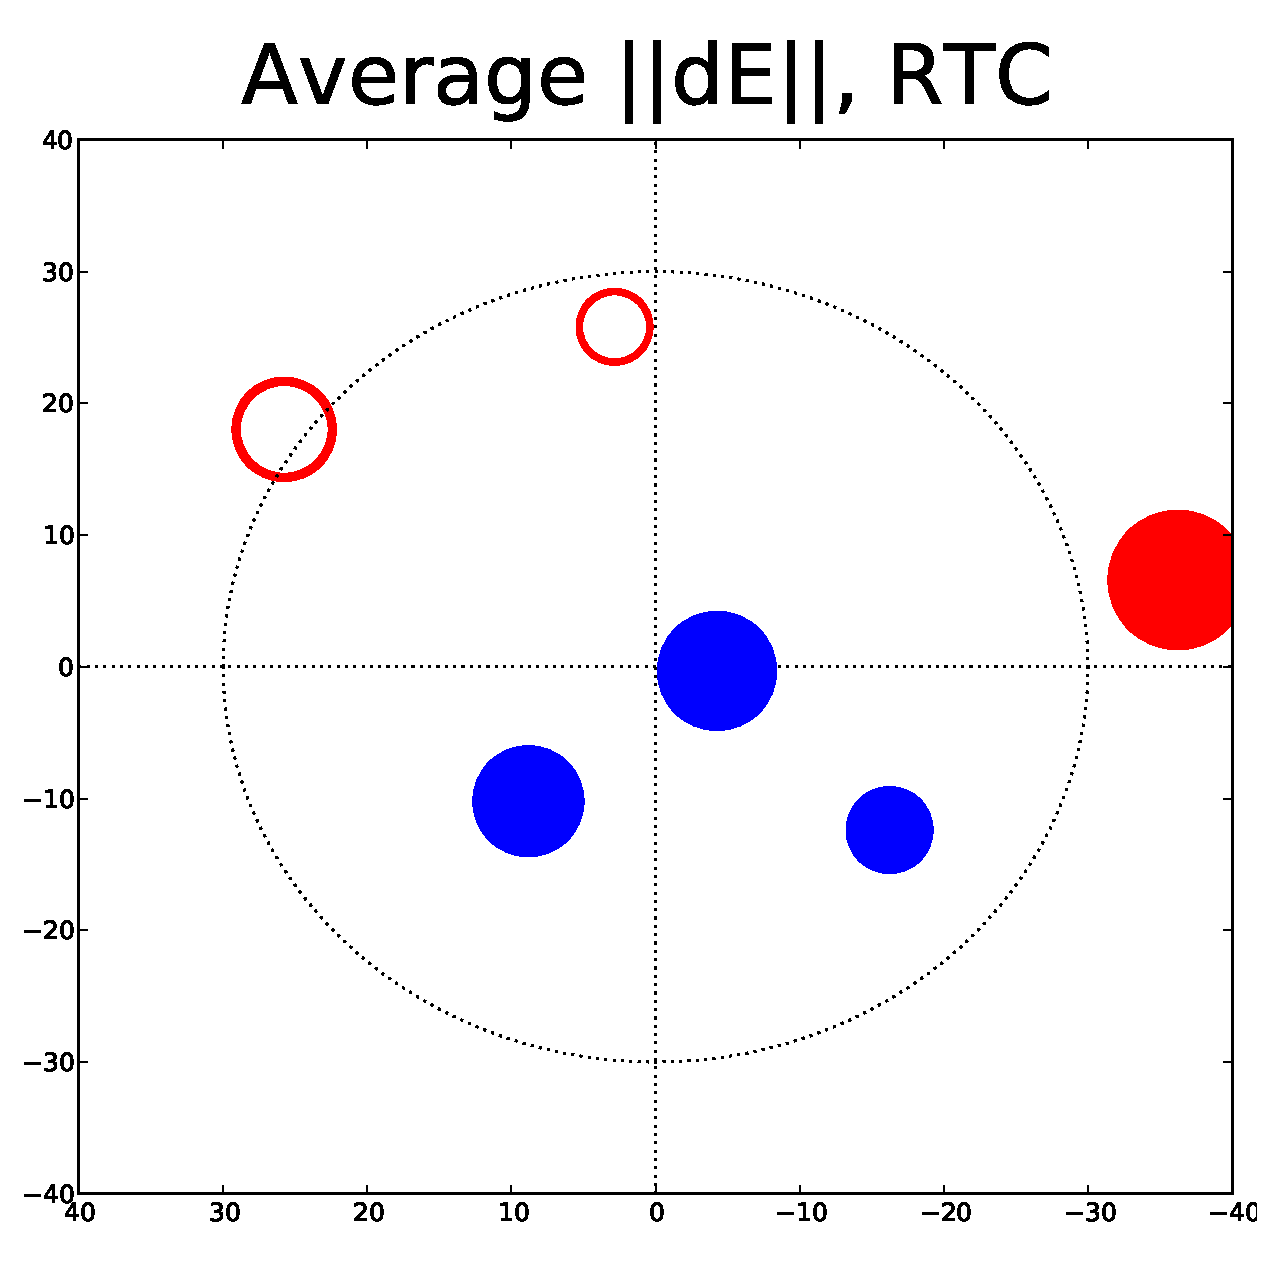
\includegraphics[width=\roguewidth]{o2006_dE_antC} &
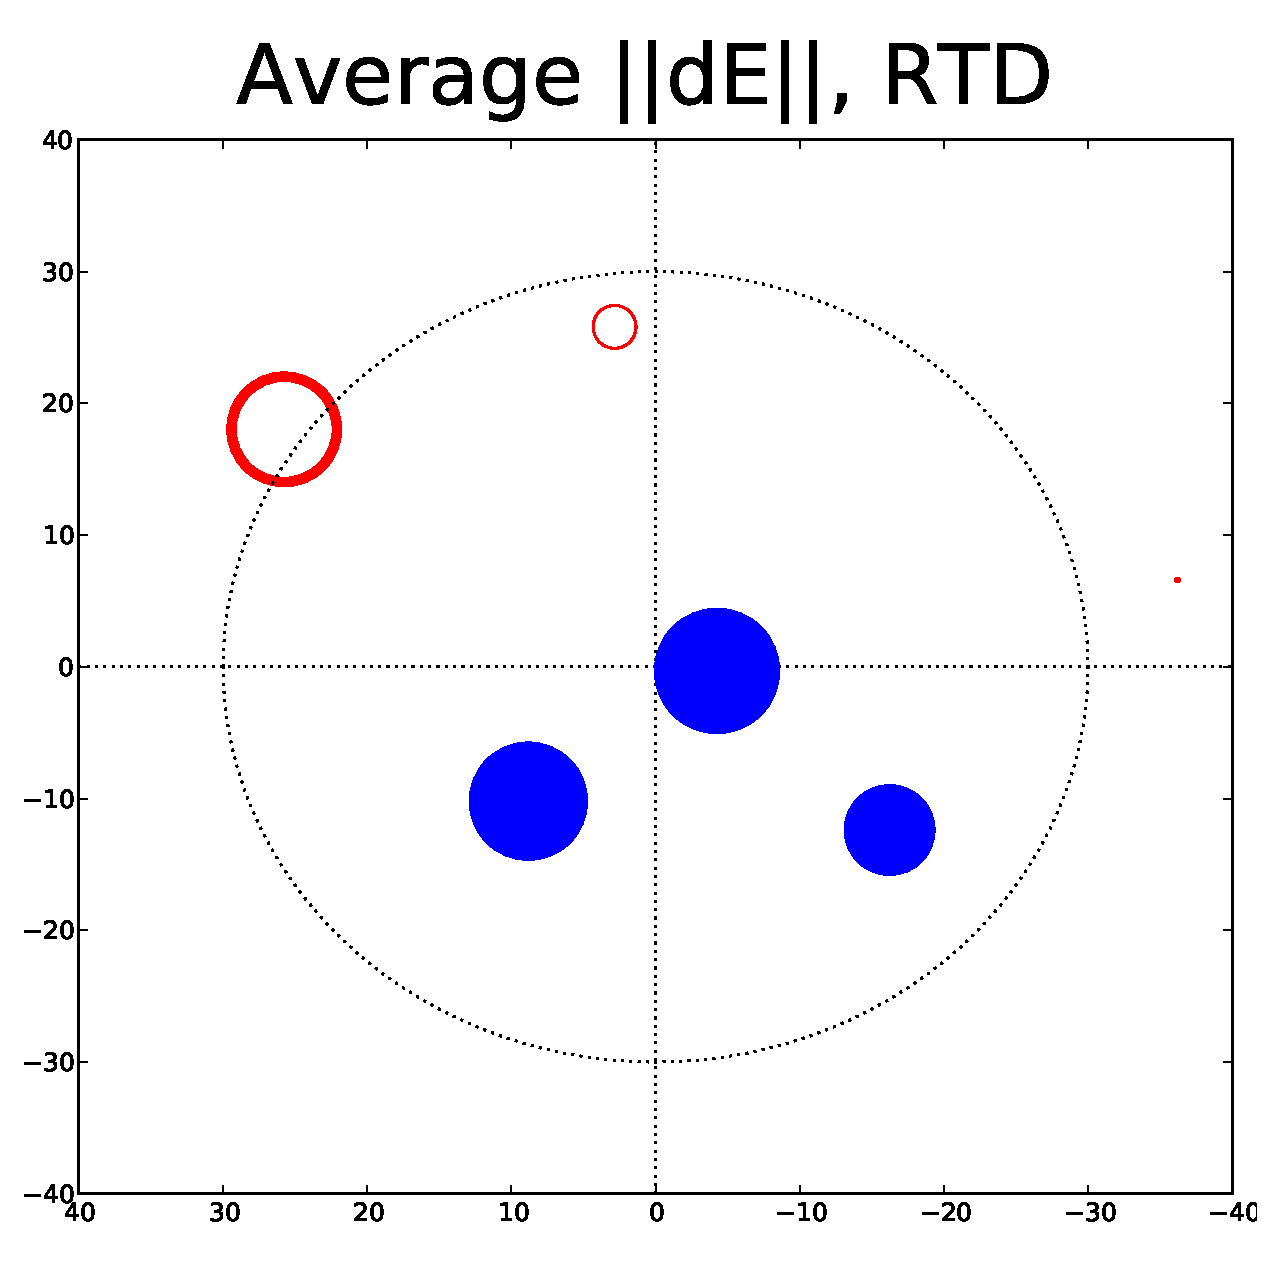
\includegraphics[width=\roguewidth]{o2006_dE_antD} 
\end{tabular}
\caption{\label{fig:rogues-2006}``Rogues gallery'' plot for the 2006 observation, using the same scale as Fig.~\ref{fig:rogues-2003}}
\end{figure}


The galleries show exactly such a pattern for antennas RT5 through RT8 (and perhaps RT4), for both the 2003 and, to a lesser extent, the 2006 observations. It is a little bit strange that 4 (or even 5) adjacent antennas would so consistently mispoint North, and do the same three years later. Perhaps this is another, poorly understood consequence of unmodelled source structure. (Note that antennas RT4--8, being in the middle of the array, form up predominantly shorter baselines; while the long-baseline antennas RTC and RTD suggest a somewhat opposite picture. It is perhaps unfortunate that the three sources exhibiting complicated structure all lie in the bottom half of the field.) Another puzzling feature is the consistently low $||\Delta\jones{E}{}||$ for sources F, H and K on antenna RTC in 2003 (and to a far lesser extent in 2006). If due to source structure, why does it not repeat on RTD? Perhaps RTC is mispointing to the South?

Antennas RT0--2, RT9 and RTA, on the other hand, show completely different patterns, with little to no similarity between 2003 and 2006. Some of these are consistent with a static mispointing. Some antennas (RT8 and RT9, and RTB especially) also show a hint of time variability in $||\Delta\jones{E}{}||$.

In any case, it is clear that the complicated interaction between source structure and differential gain-amplitudes makes the latter extremely difficult to interpret. Note also that our source model was built by NEWSTAR based on regular selfcal, so there's bound to be some contamination from DDE-related artifacts in the source parameters. Robust methods for disentangling source structure from DDEs have yet to be developed!

\subsubsection{Phase behaviour}

%for t in o2003 o2006; do plot-de-solutions.py --phase-slope -o eps -r --portrait --title-fontsize 0 -W 290 -H 40 --borders 0.03,1.12,0.01,1.6 --circle-borders 0.01,0.99,0.01,0.99 $t.cache --phase-slope-dlm --phase-slope-time-offset -0.096 --output-prefix $t; done

\begin{figure}
\centering
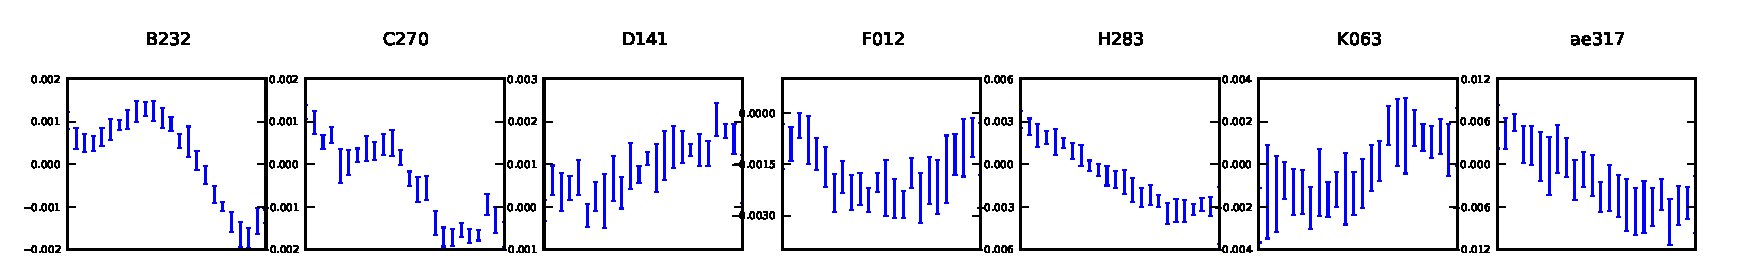
\includegraphics[width=\columnwidth]{o2003_dEphase_array_slopes}\\
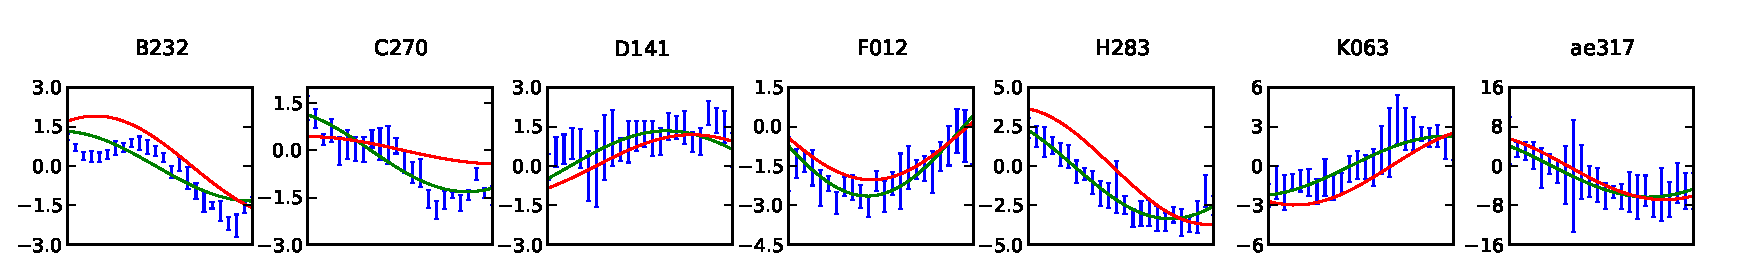
\includegraphics[width=\columnwidth]{o2006_dEphase_array_slopes}
\caption{\label{fig:dEphase-slope}Phase slopes over the array as a function of time (in deg/m) in the direction of the seven sources for the 2003 (top) and 2006 observations (bottom). The green lines indicate phase slopes corresponding to the fitted position offsets (Fig.~\ref{fig:dEphase-dlm}), the red lines -- phase slopes corresponding to an overall field rotation of $45\arcsec$.}
\end{figure}

%for t in o2003 o2006; do plot-de-solutions.py --phase-slope -o eps -r --portrait --title-fontsize 0 $t.cache --phase-slope-time-offset -0.096 --output-prefix $t --label-fontsize 20; done
\begin{figure}
\centering
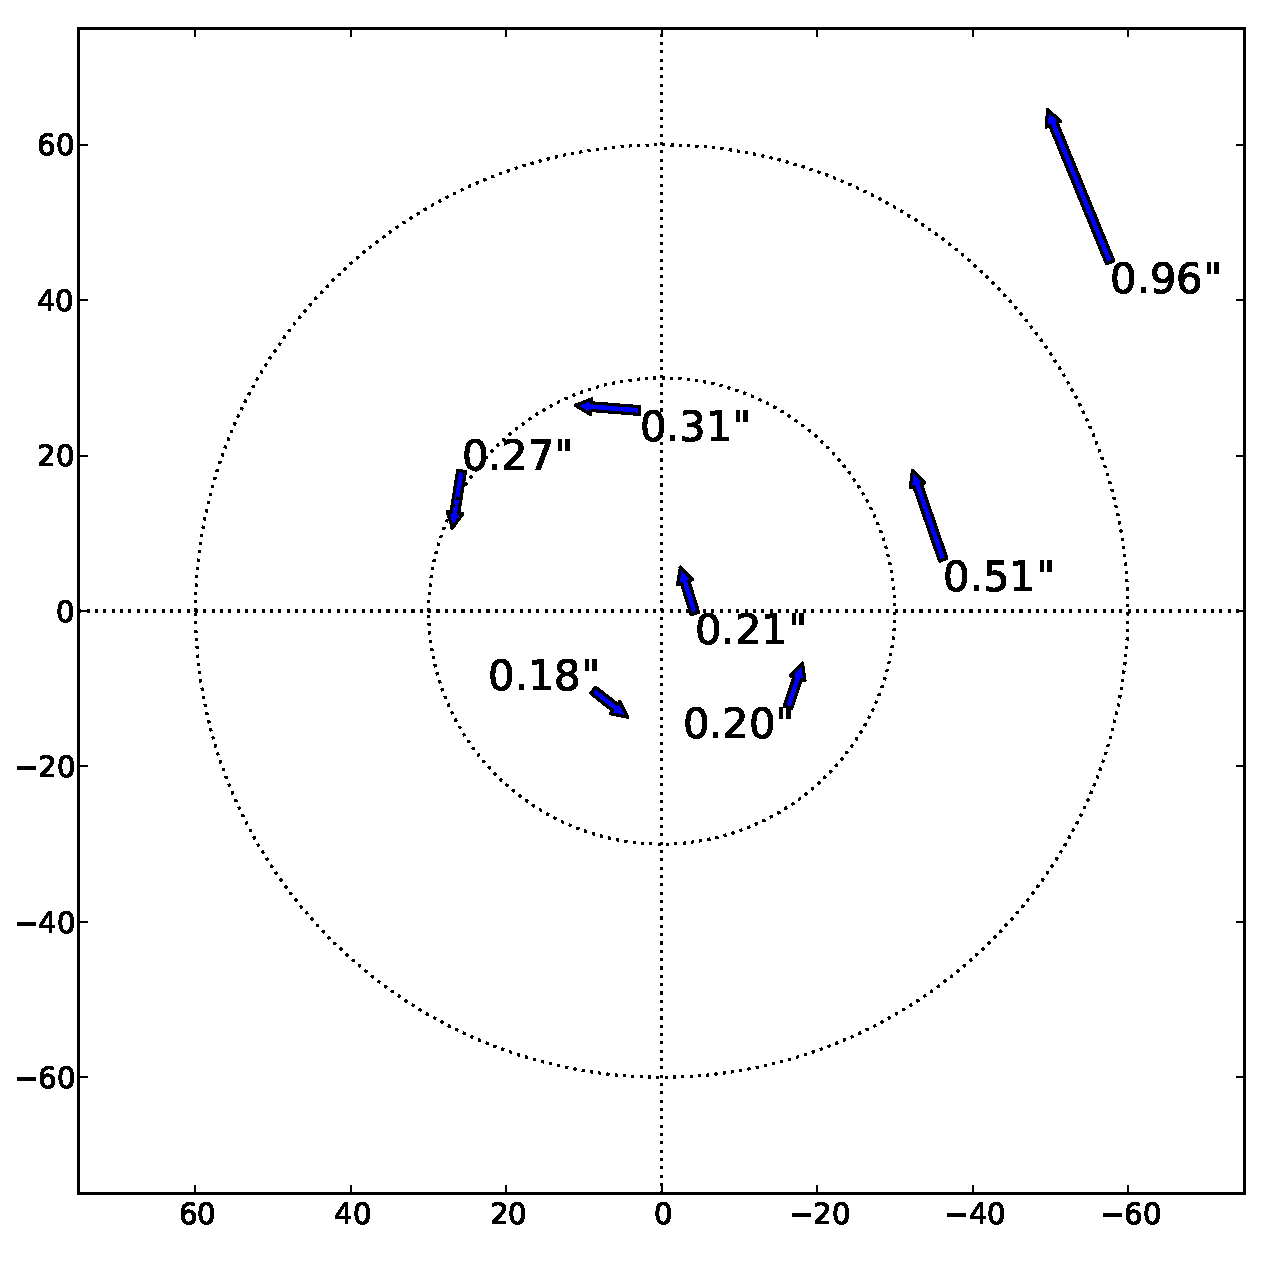
\includegraphics[width=.5\columnwidth]{o2003_dE_lm_offsets}%
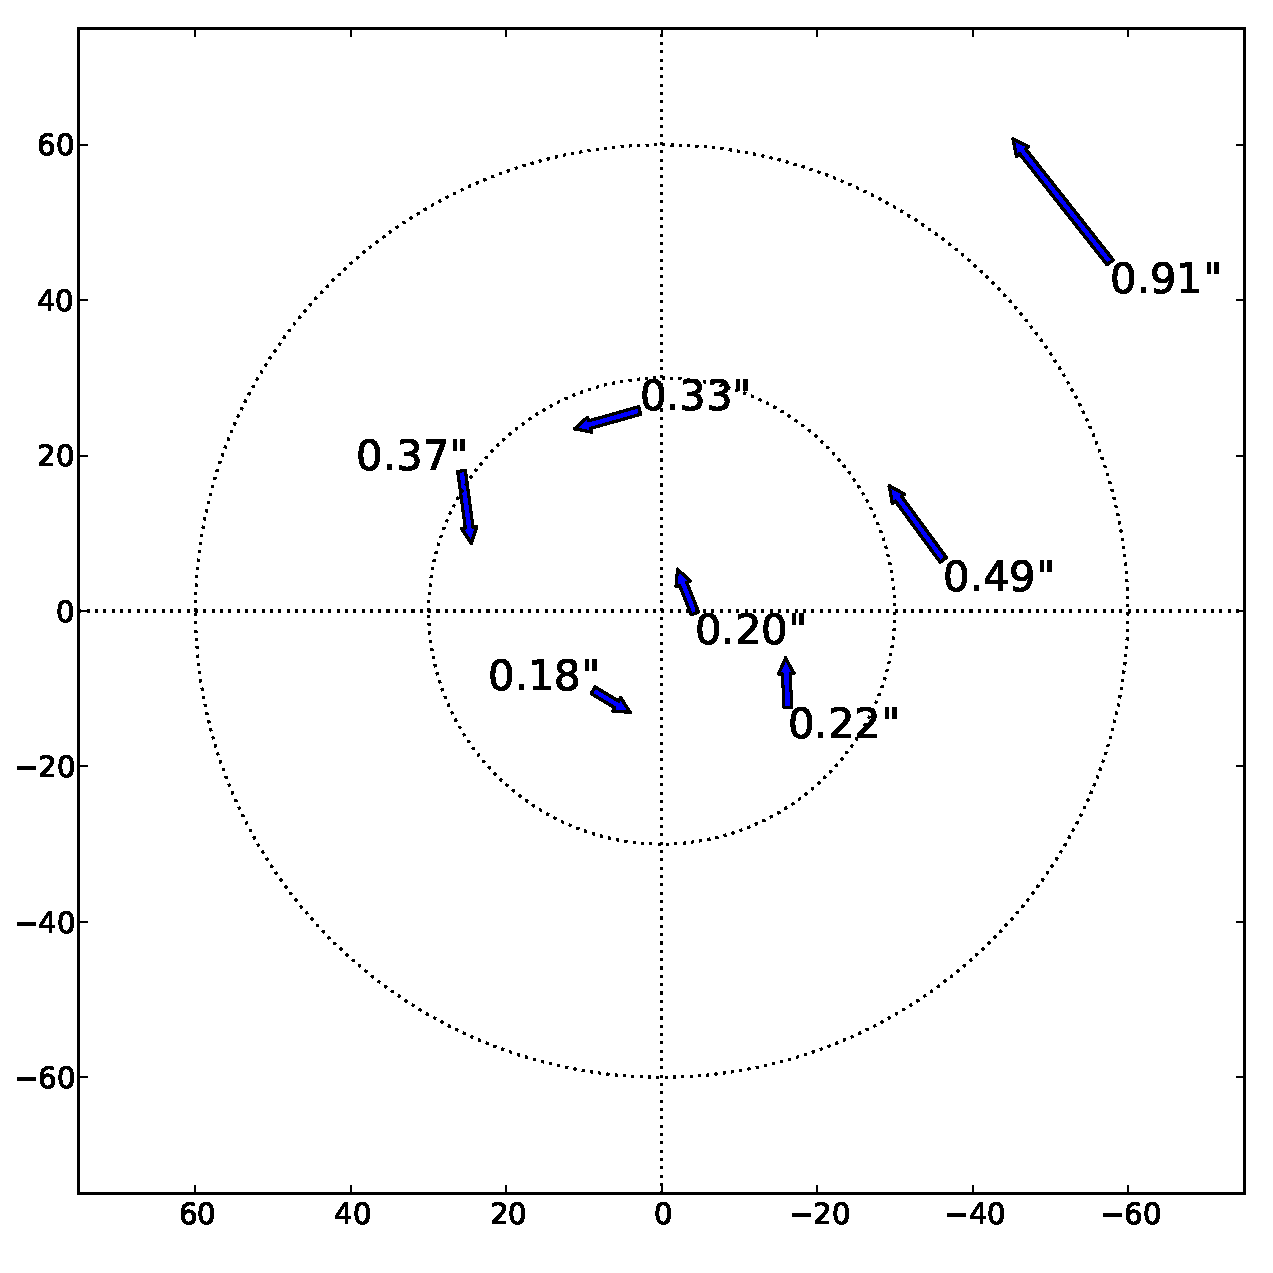
\includegraphics[width=.5\columnwidth]{o2006_dE_lm_offsets}\\
\caption{\label{fig:dEphase-dlm}Fitted position offsets corresponding to the phase slopes of Fig.~\ref{fig:dEphase-slope} (2003 observation on the left, 2006 on the right). Arrows are not to scale: the biggest offset is in fact just under $1\arcsec$.}
\end{figure}

A rather prominent feature of the phase plots in Fig.~\ref{fig:dEphase} is their continuity from antenna to antenna, and the fact that the phases at the two ends of the array exhibit opposite temporal trends. This is suggestive of an evolving phase slope over the array. Fitting such a slope (per source) produces some very striking results (Figs.~\ref{fig:dEphase-slope} and \ref{fig:dEphase-slope-res}). The dominant phase effect is clearly global rather than antenna-based, and is extremely consistent across both observations.

A phase slope over the array can be interpreted as an apparent position offset. It appears that the slope behaviour in Fig.~\ref{fig:dEphase-slope} can be fitted quite well by \emph{constant} position offsets. 
The best-fitting position offsets are indicated in Fig.~\ref{fig:dEphase-dlm}, and the corresponding slope curves are plotted in green on Fig.~\ref{fig:dEphase-slope}. 

Figure~\ref{fig:dEphase-dlm} immediately suggests a field rotation. And indeed, the entire collection of phase slopes (for both the 2003 and 2006 observation), is, to first order, consistent with a rotation of $45\arcsec$ around the phase centre. The corresponding slope curves are plotted in red. While there are some significant differences in the brighter sources, it seems clear that the dominant effect is not an instrumental DDE at all, but a systematic rotation of the sky model. The model positions are derived by NEWSTAR from direct fits to the visibilities, and de Bruyn (priv. comm.) has independently verified them to precisions of .... Note that a $45\arcsec$ rotation can also be introduced by a clock error of about 2.9 s, or a corresponding rotational error in conversion of UVW coordinates from apparent to J2000. Since NEWSTAR and MeqTrees use completely different toolchains and visibility data formats, we cannot exclude a coordinate conversion error somewhere along the line. This needs to be urgently investigated. If indeed the entire sky model is slightly rotated, then perhaps the image of Fig.~\ref{fig:3C147} can be further improved upon!

The brighter sources B, C, and (to a lesser extent) D show second-order effects that significantly deviate from the fitted slopes. This is where we should look for the ``true'' DDEs, though unmodelled source structure leaking into the phases cannot be discounted either. 

\subsection{Feeding differential gains back into the sky model\label{sec:model-improvement}}

The results above suggested we could improve our sky model by feeding back in some information extracted from the $\Delta\jones{E}{}$ solutions. In the previous section, we obtained a correction to the model positions of  the seven sources.\footnote{For the moment, we've left aside the issue of whether the positional offsets are ultimately due to a global field rotation. Improving the positions of seven of the brightest off-axis sources should already produce an superior sky model.} Section~\ref{sec:de-analysis-model} suggests that we could also provide corrections for the $I$ and $Q$ fluxes by applying the per-source average $\Delta\jones{E}{}$ amplitudes:

\begin{eqnarray*}
\coh{B}{s}^\mathrm{(corr)} & = & \overline{|\Delta\jones{E}{s}|} \coh{B}{s} \overline{|\Delta\jones{E}{s}|} \\
\overline{|\Delta\jones{E}{s}|} & \equiv & \matrixtt{\overline{|\Delta e_{xs}|}}{0}{0}{\overline{|\Delta e_{ys}|}} = \frac{1}{N_\mathrm{ant}N_t N_\nu} \sum_{p,i,j} |\Delta\jones{E}{sp}(t_i,\nu_j)|,
\end{eqnarray*}

where $t_i$ and $\nu_j$ represent the time and frequency solution intervals of $\Delta\jones{E}{}$. In terms of the $I$ and $Q$ fluxes, the correction becomes:

\begin{eqnarray*}
I^\mathrm{(corr)} = \Sigma \cdot I + \Delta \cdot Q, & \; &  Q^\mathrm{(corr)} = \Delta \cdot I + \Sigma \cdot Q, \\
\Sigma = \frac{1}{2}\left( \overline{|\Delta e_{xs}|}^2 + \overline{|\Delta e_{ys}|}^2 \right), 
& \; & \Delta = \frac{1}{2}\left( \overline{|\Delta e_{xs}|}^2 - \overline{|\Delta e_{ys}|}^2 \right).
\end{eqnarray*}

We therefore applied these corrections for $I$, $Q$, and position to our sky models (independently for the 2003 and 2006 observations), and repeated the calibration procedure. An improvement in single-band residuals was immediately apparent (Fig.~\ref{fig:residuals-newmodel}) -- after $\jones{G}{p}$ and $\coh{M}{pq}$ solutions, the seven off-axis sources subtracted noticeably better. Single-band residuals after $\Delta\jones{E}{sp}$ solutions, on the other hand, look pretty much the same (this is not surprising, since differential gains had already taken care of the off-axis sources in the original reduction), with a very slight improvement around 3C147 itself, which can be explained by improved $\jones{G}{p}$ solutions due to the more accurate sky model.

\begin{figure}
\begin{centering}
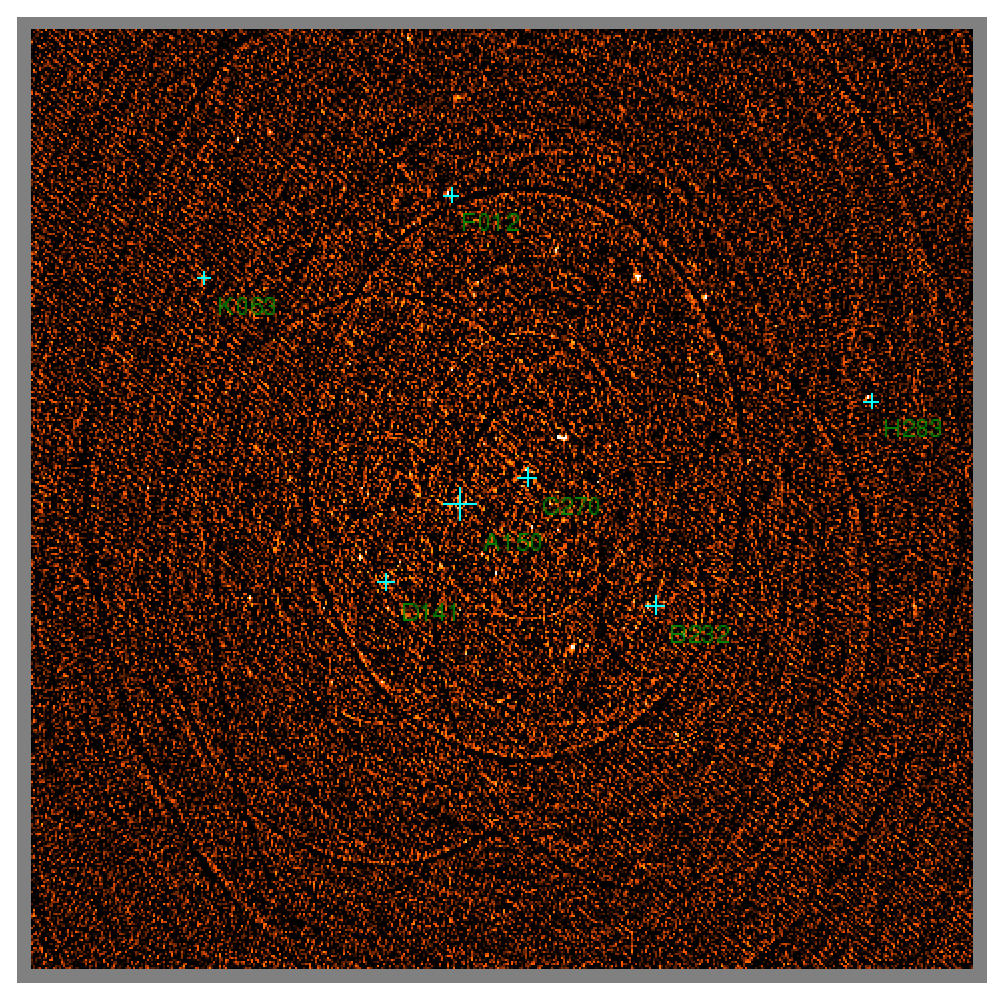
\includegraphics[width=.5\columnwidth]{spw2_oldmodel}%
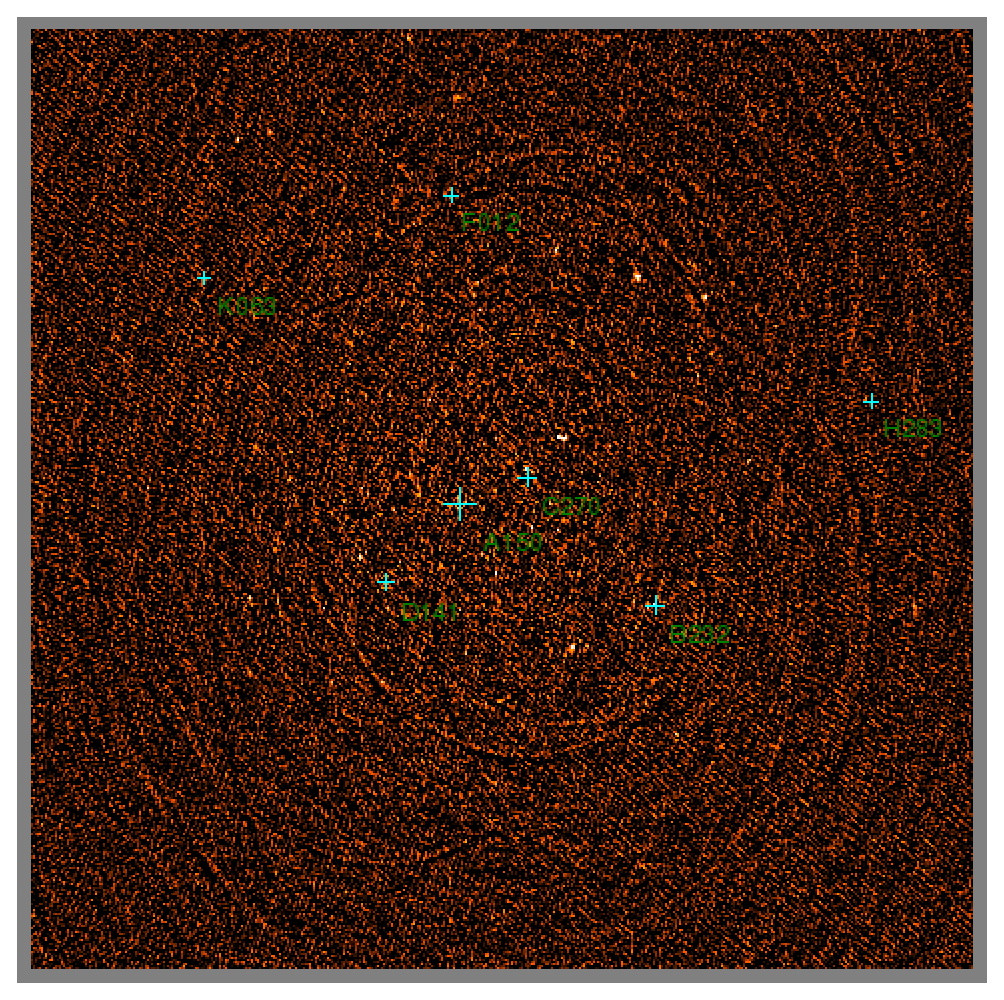
\includegraphics[width=.5\columnwidth]{spw2_newmodel}\par
\end{centering}
\caption{\label{fig:residuals-newmodel}Calibration with an improved sky model. This shows single-band residual images after $\jones{G}{p}$ and $\coh{M}{pq}$ solutions. The left image is from the original reduction, the right image uses a sky model improved via our $\Delta\jones{E}{}$ analysis. Crosses indicate the positions of sources for which the model was improved, plus 3C147 itself (source A).}
\end{figure}

Presumably, the remaining residual structures in Fig.~\ref{fig:residuals-newmodel} are more representative of the DDEs themselves, since inaccuracies in the sky model have been significantly reduced. We would also expect the differential gain solutions to be more indicative of the actual DDEs (apart from the issue of resolved sources affecting $||\Delta\jones{E}{}||$ on antennas RTC and RTD, which the improved sky models do not address at all.)




%plot-de-solutions.py --phase-slope-res -o eps -r --portrait --title-fontsize 0 -W 290 -H 100 --borders 0.02,1.02,0.01,1.08 MS/3C*/dE*
%plot-de-solutions.py --phase-slope-res -o eps -r --portrait --title-fontsize 0 -W 290 -H 100 --borders 0.02,1.02,0.01,1.08 MS/m30*/dE* --output-prefix o2006

\begin{figure*}
\sidecaption
\parbox[b]{12cm}{
\includegraphics[width=12cm]{dEphase_array_slopes_res}
\includegraphics[width=12cm]{o2006_dEphase_array_slopes_res}
}
\caption{\label{fig:dEphase-slope-res}Residual phases w.r.t. slope fits.}
\end{figure*}


\section{Conclusions}

Since its original formulation by \citet{ME1}, the Radio Interferometer Measurement Equation (RIME) has 
provided the mathematical underpinnings for novel calibration methods and algorithms. Several authors have developed carious approaches to the DDE problem based on the RIME. Different versions of the formalism have been used for this: they are mathematically equivalent, and have been reformulated into one consistent framework within this paper. Besides its explanatory power, the RIME formalism can be wonderfully simple and intuitive; this 
fact has become somewhat obscured by the many different directions that it has been developed in. It is hoped that the first part of this paper has gone some way to making the RIME simple again. Finally, a number of misunderstandings and controversies has inevitably accrued themselves to the formalism over the years. Some of these have been addressed here .

Besides its obvious explanatory ability, one of the biggest selling points of the RIME formalism is the flexibility it offers for describing observational effects. Unfortunately, to date only three software packages have exploited the power of the RIME (CASA, MeqTrees, and the LOFAR BBS system). Of these, only MeqTrees allows for truly arbitrary forms of the RIME. This paper has explored some practical applications of one such form of the RIME: a form that includes differential gain terms.

We have demonstrated that the differential gain approach (the ``flyswatter'') can be a powerful way of dealing with DDEs on a source-by-source basis. This has been used with WSRT data to produce artifact-free maps of 3C147 at record dynamic ranges of well over a million-to-one. While the differential gain solutions themselves absorb inaccuracies in the sky model as well as the DDEs themselves, we have demonstarted that at least flux and positions corrections can be recovered, so iterative improvements to the sky model are possible.

The nature of the remaining DDEs (as seen in the differential gain solutions) has not yet been adequately explained. Some of the amplitude effects are consistent with pointing error. There phase behaviour is even more difficult to understand, but may be due to unmodelled source structure. Further work is required on the subject. 

We have shown that differential gain-phase solutions can be used to detect position shifts to within small fractions of the synthesized beam size. Offsets as small as $0.2\arcsec$ have been reliably detected. There is a very clear indication of a systematic rotational offset of $\sim45\arcsec$ in the sky model generated by NEWSTAR, when interpreted using MeqTrees. This is may be due to a coordinate conversion error somewhere in the visibility data processing toolchain, and needs to be investigated further.

Finally, we should consider some wider implications of our results. All currently mooted schemes of DDE calibration for LOFAR \citep{JEN:LOFAR3}, the MWA \citep{Mitchell:MWA-cal} and the ionosphere in general \citep{Intema:SPAM,Cotton:FBC} revolve around the use of ``beacon sources'' to probe the ionosphere and/or the primary beam. It is rather difficult to envisage a closed-loop scheme without beacons (how else would one sample a DDE?), so future telescopes such as the SKA will most likely need to use something very similar. Any such scheme predicates on there being a sufficient number of sufficiently bright in-beam beacons for any direction on the sky. This is not a problem at the LOFAR and MWA end of the spectrum, since the low-frequency sky is so much brighter, but it has been a bit of a worry for the higher frequencies, where FoVs are narrower and sources are fainter.

Our 3C147 results suggest that calibration beacons can be a lot fainter than previously thought. What has been established is that for this particular configuration of the WSRT, sources as faint as 2~mJy can provide meaningful DDE solutions. This result can be scaled to future telescope designs by comparing their expected sensitivity with that of the 3C147 observation.

\bibliographystyle{aa}

\bibliography{me6_dde}


\end{document}